% Archivo generado desde ../documento_final.docx.
% Edite el DOCX maestro o este archivo según el flujo de trabajo acordado.

\section*{Fundamentación del programa}

\subsection*{Objeto de estudio.}

En nuestra vida diaria, dependemos en gran medida de numerosos sistemas electromecánicos. Casi toda la generación de electricidad es impulsada por máquinas electromecánicas, específicamente generadores, que convierten diversas formas de energía, como la nuclear, hidráulica, térmica, oceánica y eólica, en energía eléctrica. Además, la mayoría de las máquinas, equipos y dispositivos que facilitan las tareas diarias realizadas por los humanos son sistemas electromecánicos.\par

Algunos ejemplos de sistemas electromecánicos presentes en aplicaciones de uso diario son:\par

\begin{itemize}
\item Discos duros magnéticos
\item Alternadores de vehículos de combustión
\item Sistemas de tracción en vehículos eléctricos a batería
\item Micrófonos capacitivos para computadoras y teléfonos inteligentes
\item Acelerómetros micro fabricados para teléfonos inteligentes
\item Electrodomésticos y herramientas eléctricas
\item Elevadores y escaleras mecánicas
\item Cámaras de refrigeración de supermercados
\item Aires acondicionados en hogares y oficinas
\end{itemize}
Las personas ingenieras electromecánicas idean y diseñan nuevos sistemas electromecánicos, además de utilizar y mantener los ya existentes. El programa de Ingeniería Electromecánica tiene como objeto de estudio los sistemas electromecánicos. Las áreas de conocimiento que habilitan en el estudio de los sistemas electromecánicos y sus respectivos saberes juntos con su peso porcentual se muestran en la Figura\textbf{ }3 y además se definen en la siguiente lista:\par

\begin{itemize}
\item \textbf{Ciencias Básicas:} comprende el conocimiento fundamental en matemáticas, física y química, esenciales para el desarrollo de habilidades analíticas y la comprensión de los principios que sustentan la ingeniería.
\item \textbf{Formación Profesional y Habilidades Interpersonales:} abarca las competencias éticas, sociales y laborales, así como el liderazgo, emprendimiento y administración de proyectos.
\item \textbf{Comunicación y Dibujo: }comprende lo relacionado con la comunicación de ideas de manera efectiva, tanto oralmente como por escrito, y el uso del dibujo para la representación gráfica en la ingeniería.
\item \textbf{Ingeniería Eléctrica y Electrónica:} abarca los circuitos, máquinas eléctricas y electrónica, áreas fundamentales para la operación y diseño de sistemas electromecánicos.
\item \textbf{Ingeniería Mecánica y de Materiales:} comprende el estudio de materiales y su comportamiento, así como los principios de la mecánica, termodinámica y manufactura aplicados en el diseño y análisis de sistemas mecánicos.
\item \textbf{Automática:} incluye la programación, el control y la automatización de sistemas, incluyendo modelado y simulación, lo que permite optimizar procesos y mejorar la eficiencia de los sistemas electromecánicos.
\item \textbf{Análisis de Datos:} se centra en el uso de estadísticas, metrología y diseño de experimentos para la recopilación, análisis e interpretación de datos, cruciales para la toma de decisiones en el ámbito de la ingeniería.
\end{itemize}
\subsubsection*{Distribución de saberes y áreas disciplinares para el tronco común (Total: 75\%)}

En la siguiente lista, el primer nivel representa las áreas disciplinares y el segundo nivel representa los saberes dentro de esas áreas disciplinares. Se muestra en cada una de las áreas y cada uno de los saberes su peso porcentual en la Licenciatura en Ingeniería Electromecánica, esto considerando que el tronco común corresponde a un 75\% del total de créditos de la Licenciatura. En la Figura 3 se incluye un gráfico de radar que muestra la distribución porcentual de saberes por área.\par

\begin{enumerate}
\item Ciencias Básicas (19.9\%)
\begin{enumerate}
\item Matemática (11.6\%)
\item Física (6.1\%)
\item Química (2.2\%)
\end{enumerate}
\item Formación profesional y habilidades interpersonales (7.7\%)
\begin{enumerate}
\item Ética y ciencias sociales (3.6\%)
\item Habilidades interpersonales (0.8\%)
\item Emprendedurismo (2.2\%)
\item Administración de proyectos (1.1\%)
\end{enumerate}
\item Comunicación y dibujo (5.6\%)
\begin{enumerate}
\item Comunicación oral y escrita (1.7\%)
\item Inglés (0.6\%)
\item Dibujo para ingeniería (3.3\%)
\end{enumerate}
\item Ingeniería eléctrica y electrónica (13.1\%)
\begin{enumerate}
\item Circuitos eléctricos y electrónica (6.6\%)
\item Máquinas eléctricas (4.4\%)
\item Instrumentación y transductores (2.1\%)
\end{enumerate}
\item Ingeniería mecánica y de materiales (18.3\%)
\begin{enumerate}
\item Ciencia e ingeniería de los materiales (1.7\%)
\item Mecánica de sólidos y fluidos (7.2\%)
\item Termodinámica y transferencia de calor (5.5\%)
\item Elementos de máquinas (1.7\%)
\item Manufactura (2.2\%)
\end{enumerate}
\item Automática (7.9\%)
\begin{enumerate}
\item Programación (0.6\%)
\item Modelado y simulación (1.7\%)
\item Microcontroladores y arquitectura de computadores (1.7\%)
\item Sistemas de control y automatización (3.9\%)
\end{enumerate}
\item Análisis de datos (2.5\%)
\begin{enumerate}
\item Estadística y diseño de experimentos (1\%)
\item Confiabilidad, disponibilidad, mantenibilidad y seguridad (1\%)
\item Metrología (0.5\%)
\end{enumerate}
\end{enumerate}
\begin{figure}[H]
\centering
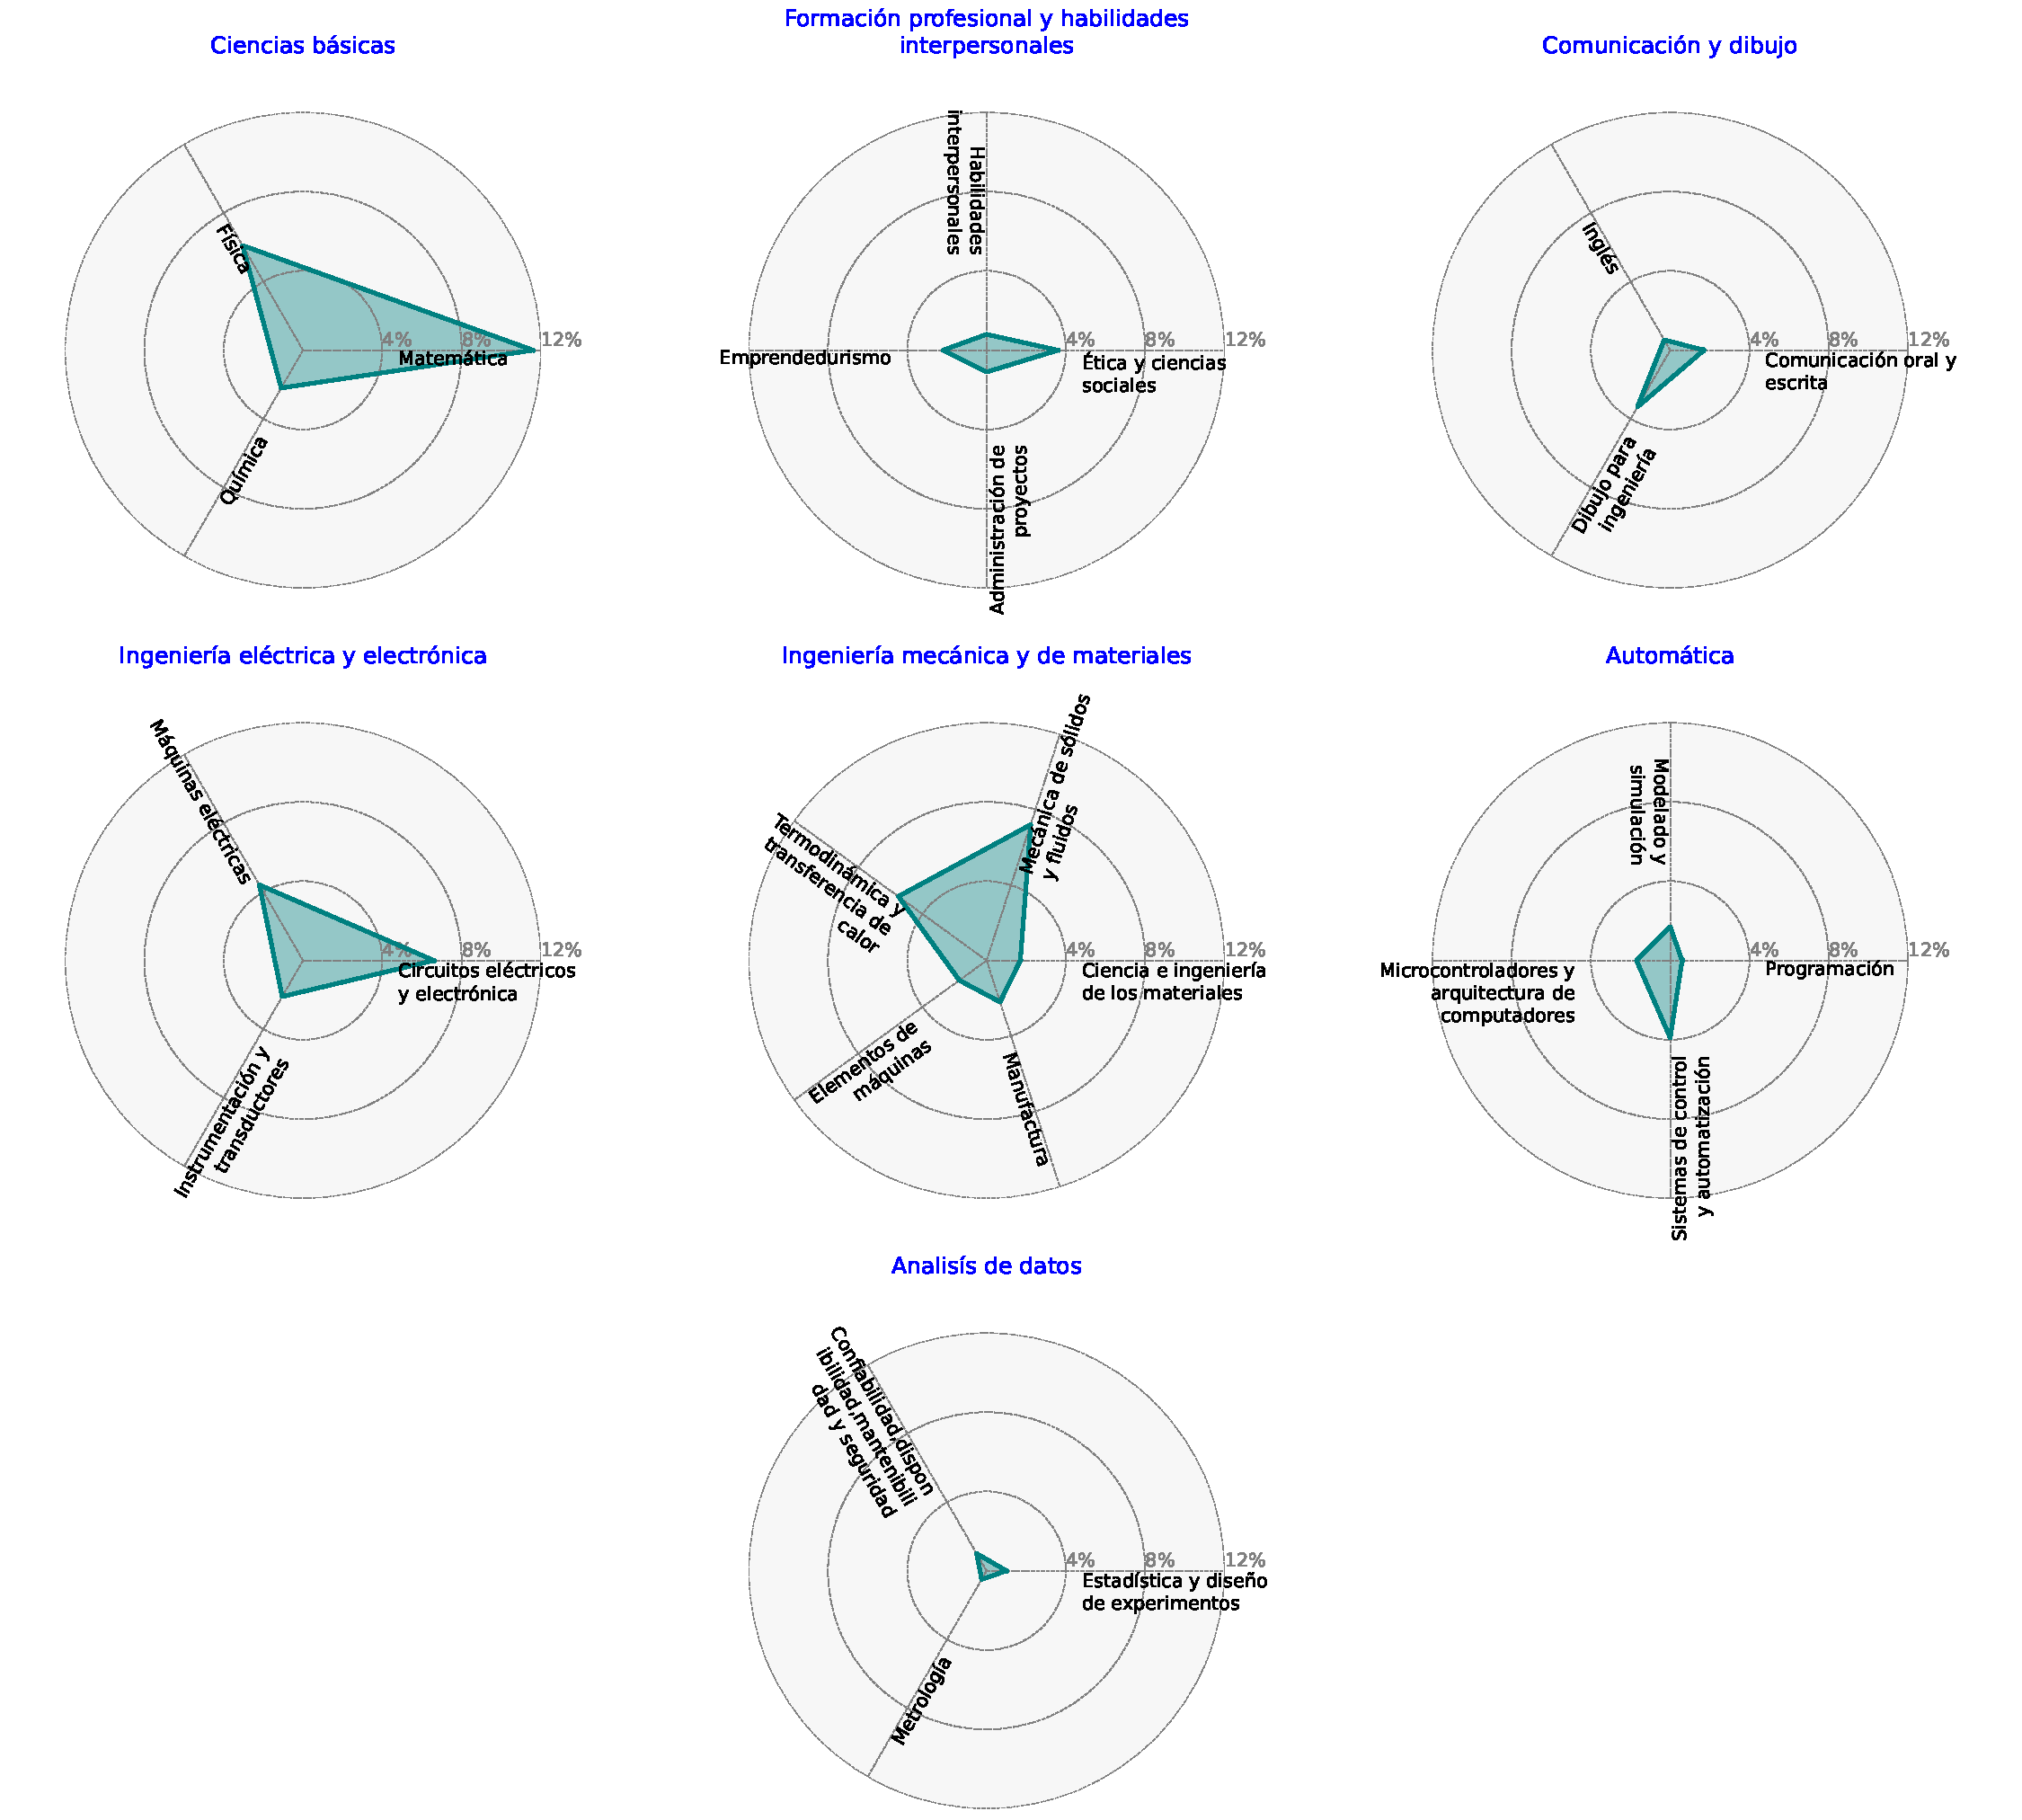
\includegraphics[width=\textwidth,height=.70\textheight,keepaspectratio]{generacion_graficos/salida/porcTRC.pdf}
\par\vspace{2mm}
{\centering\small Figura 3. Distribución porcentual de saberes dentro de las áreas disciplinares del tronco común\par}
\end{figure}

\subsection*{Sub-objetos de estudio}

El objeto de estudio del programa de Ingeniería Electromecánica son los sistemas electromecánicos, estos sistemas están presentes en todos los ambientes en los que se desarrolla el ser humano. Si nos enfocamos en diferentes sectores productivos, el tipo de sistema electromecánico tiende a especializarse al punto que requiere enfatizar en conocimientos específicos. De esta forma, el TEC busca atender necesidades de la sociedad y la industria y para ello hemos denominado en esta sección un derivado del objeto de estudio al cual llamamos sub-objetos de estudio. Es así como, desde la perspectiva de la ingeniería electromecánica, definimos tres sub-objetos que dan origen a los énfasis de la carrera:\par

\begin{itemize}
\item Instalaciones electromecánicas
\item Aeronáutica
\item Sistemas ciberfísicos
\end{itemize}
A partir de la intersección de la Ingeniería Electromecánica con los sub-objetos, se plantea el desarrollo de tres énfasis para atender esos nichos particulares. Independientemente del énfasis que se seleccione, el peso porcentual de las áreas disciplinares es el que se muestra en la Figura 4, en el que se incluye un 75\% de los créditos en el tronco común y un 25\% de los créditos en el énfasis.\par

\begin{figure}[H]
\centering
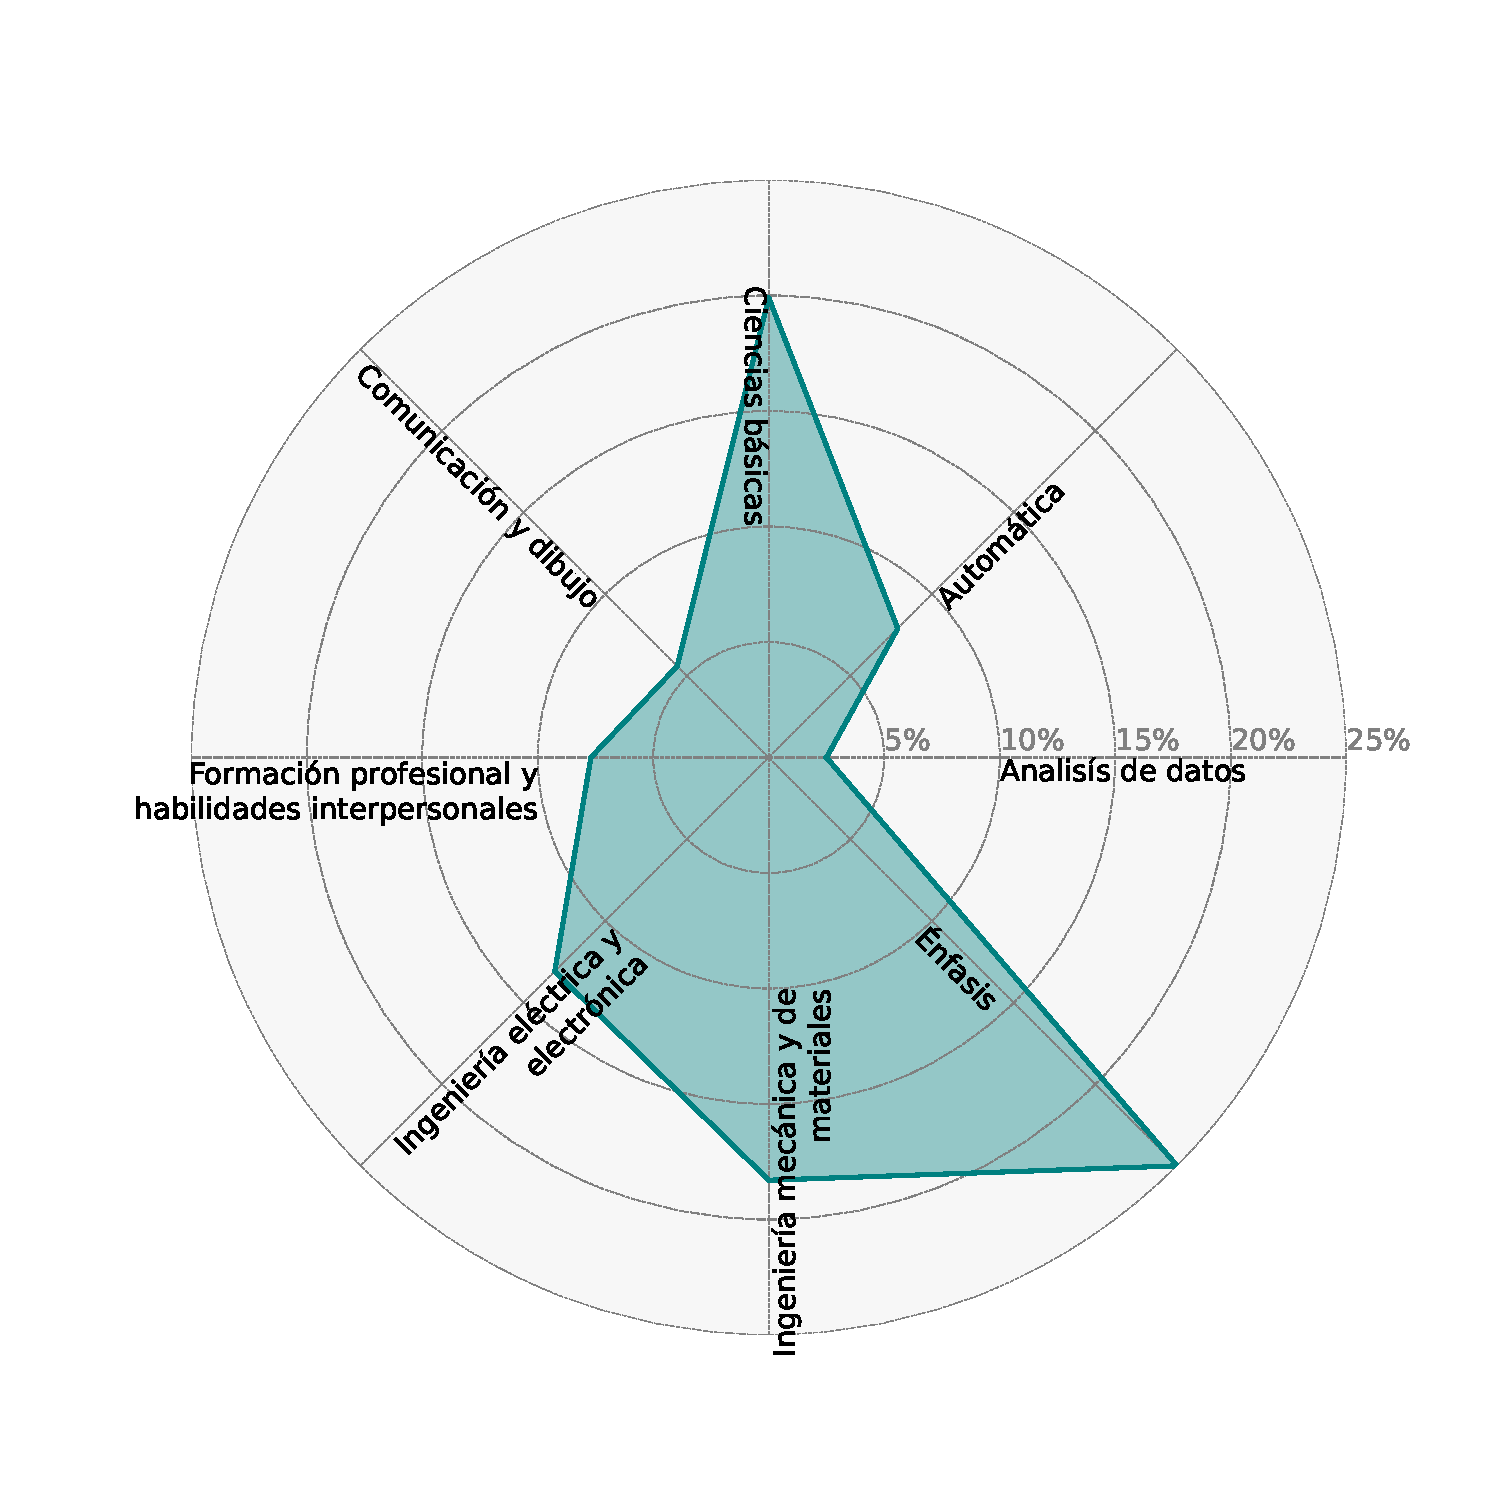
\includegraphics[width=.58\textwidth,height=.70\textheight,keepaspectratio]{generacion_graficos/salida/ENF.pdf}
\par\vspace{2mm}
{\centering\small Figura 4. Distribución porcentual de las áreas disciplinares para la Licenciatura con énfasis\par}
\end{figure}

\subsubsection*{Énfasis: Instalaciones electromecánicas.}

Este énfasis brinda herramientas para el diseño, implementación y gestión de sistemas relacionados con el transporte de masa y energía, con un enfoque particular en la energía eléctrica y mecánica en diversas instalaciones industriales, habitacionales, deportivas, hospitalarias, etc. En este énfasis se desarrollan competencias para diseñar y operar sistemas complejos que involucren la generación, almacenamiento y uso eficiente de la energía. También se trabaja en la gestión de proyectos y en la optimización a través de la transformación digital de estos sistemas.\par

La Figura 5, muestra la distribución de saberes dentro la nueva área disciplinar llamada \textit{Instalaciones electromecánicas}. La formación completa se compone de los saberes del tronco común más estos nuevos saberes mostrados en la figura.\par

\paragraph{Distribución de saberes dentro del énfasis: Instalaciones electromecánicas (25\%):}

\begin{itemize}
\item Instalaciones electromecánicas (12.2\%)
\item Sistemas de generación y almacenamiento de energía (1.9\%)
\item Sistemas de distribución y transmisión de energía eléctrica (1.9\%)
\item Gestión del ciclo de vida y transformación digital (2.6\%)
\item Gestión de la energía (1.9\%)
\item Liderazgo e inclusión (1.3\%)
\item Sostenibilidad e impacto social de la ingeniería (1.3\%)
\item Investigación y presentación de resultados (1.9\%)
\end{itemize}
\begin{figure}[H]
\centering
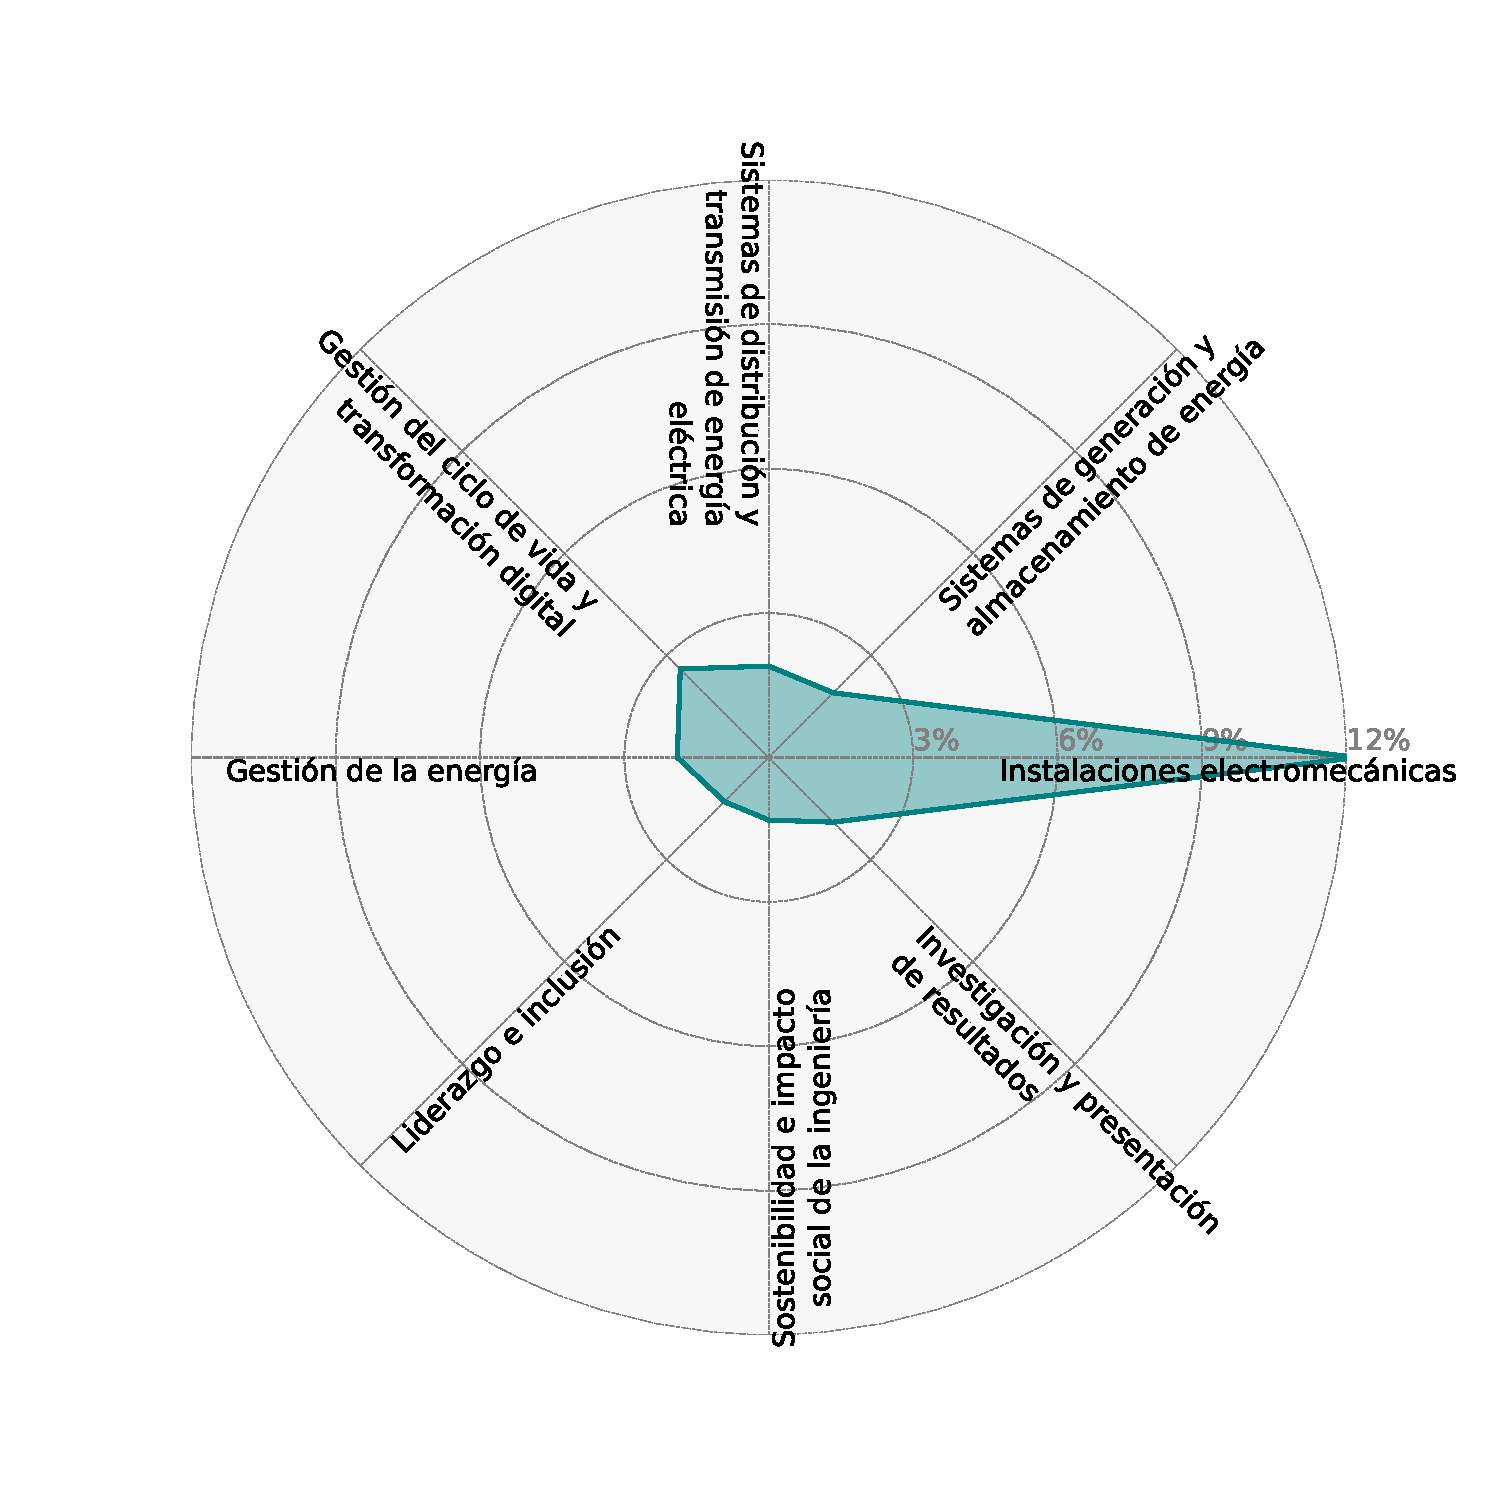
\includegraphics[width=.58\textwidth,height=.70\textheight,keepaspectratio]{generacion_graficos/salida/INS.pdf}
\par\vspace{2mm}
{\centering\small Figura 5. Distribución porcentual de saberes para el énfasis en Instalaciones electromecánicas\par}
\end{figure}

\subsubsection*{Énfasis: Aeronáutica.}

Este énfasis está\textbf{ }centrado en el diseño, desarrollo y gestión de sistemas aeronáuticos, cubriendo tanto los sistemas de control y aviónica como estructuras, mecanismos y materiales. Los estudiantes desarrollan conocimientos especializados sobre propulsión, análisis estructural y dinámica de vuelo, integrando enfoques modernos para la operación segura y eficiente de aeronaves y sus infraestructuras asociadas.\par

La Figura 6, muestra la distribución de saberes dentro de la nueva área disciplinar llamada \textit{Aeronáutica}. La formación completa se compone de los saberes del tronco común más estos nuevos saberes mostrados en la figura.\par

\paragraph{Distribución de saberes dentro del énfasis: Aeronáutica (25\%):}

\begin{itemize}
\item Aviónica, dinámica de vuelo y control de vuelo (5.8\%)
\item Aerodinámica y sistemas de propulsión (3.8\%)
\item Análisis mecánico de materiales, estructuras y mecanismos de la aeronave (5.1\%)
\item Gestión del ciclo de vida de la aeronave (3.2\%)
\item Seguridad aeronáutica y aeronavegabilidad (2.6\%)
\item Liderazgo e inclusión (1.3\%)
\item Sostenibilidad e impacto social de la ingeniería (1.3\%)
\item Investigación y presentación de resultados (1.9\%)
\end{itemize}
\begin{figure}[H]
\centering
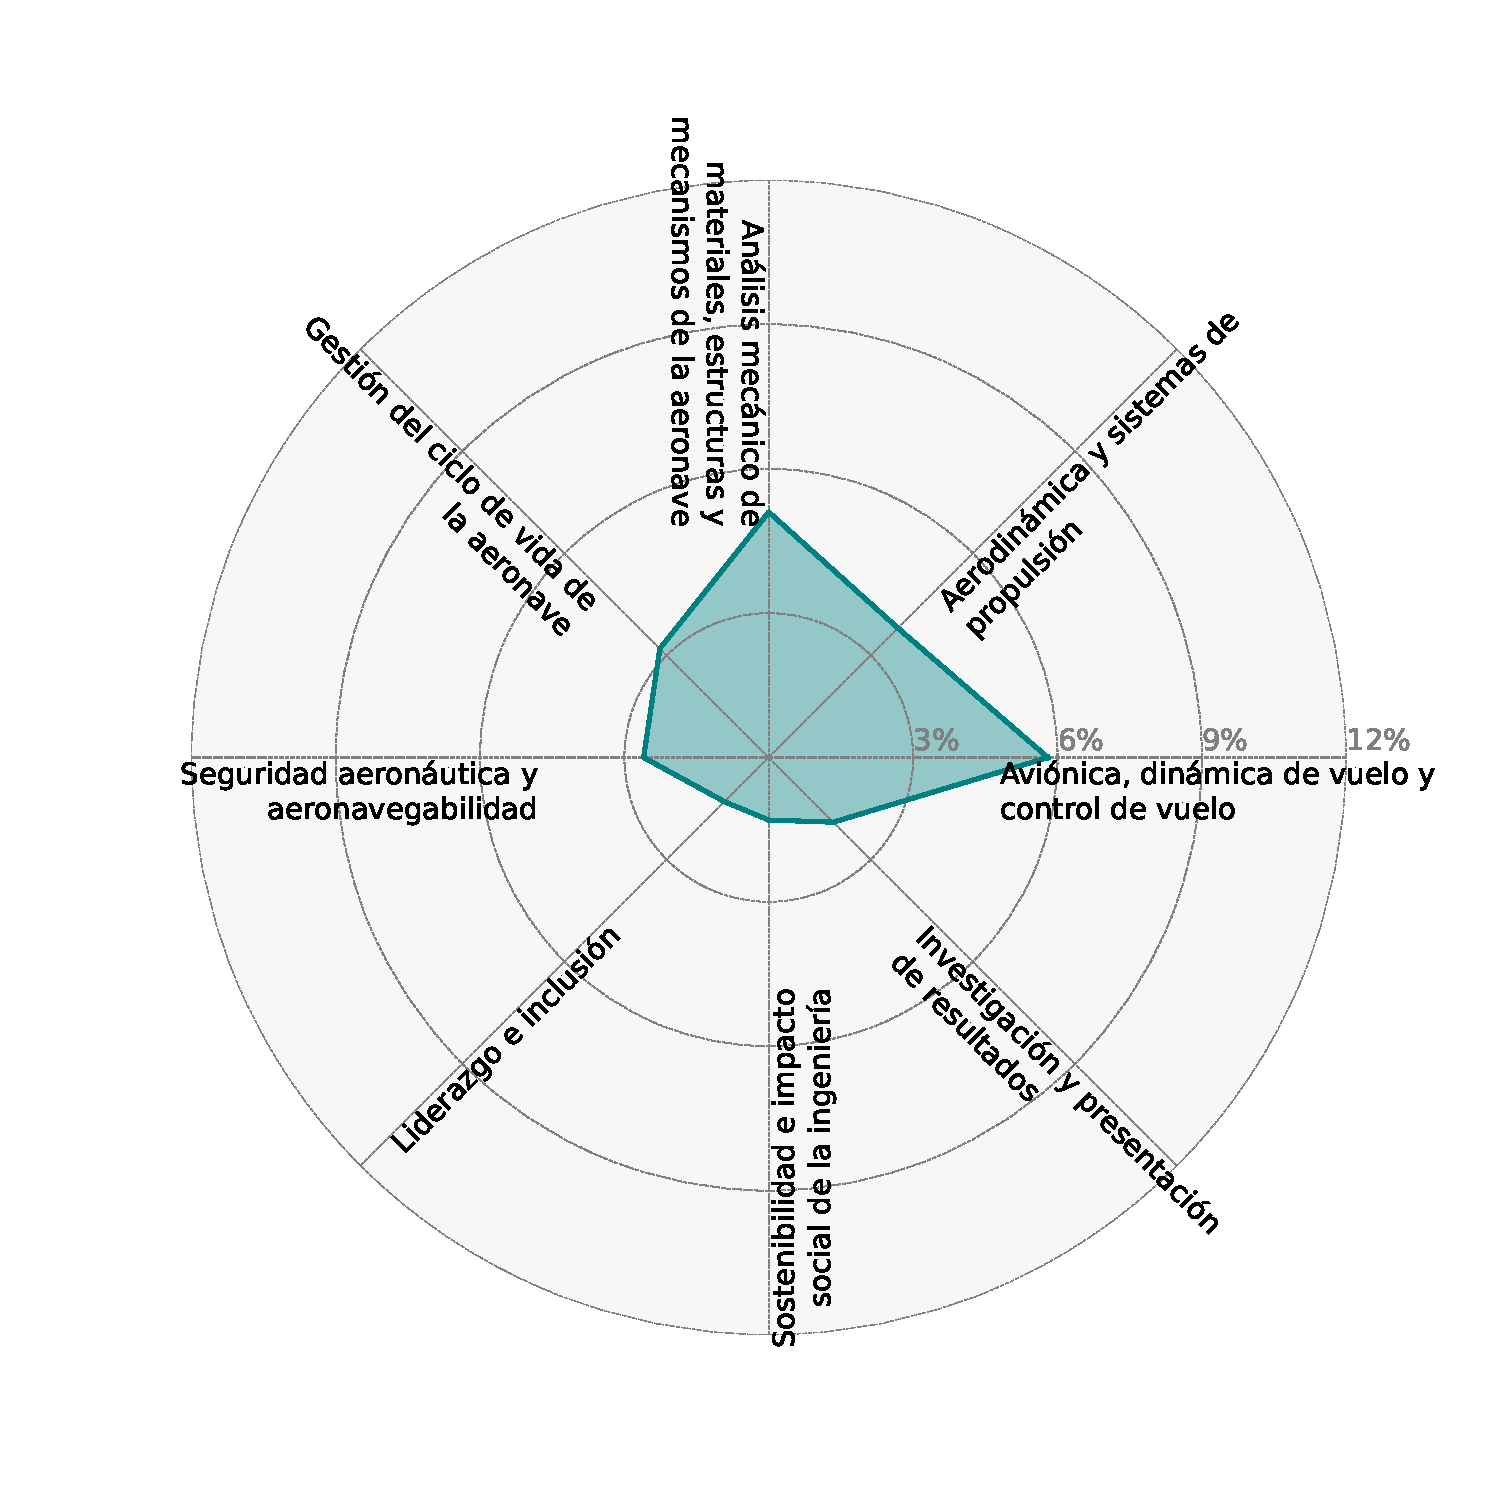
\includegraphics[width=.58\textwidth,height=.70\textheight,keepaspectratio]{generacion_graficos/salida/AER.pdf}
\par\vspace{2mm}
{\centering\small Figura 6. Distribución porcentual de saberes para el énfasis en Aeronáutica\par}
\end{figure}

\subsubsection*{Énfasis: Sistemas ciberfísicos.}

Este énfasis se enfoca en la integración de sistemas físicos con sistemas computacionales en tiempo real, con el objetivo de crear soluciones autónomas, inteligentes y seguras que interactúen con el entorno. Se introducen tecnologías como inteligencia artificial y ciberseguridad. Los estudiantes aprenderán a diseñar, desarrollar y gestionar sistemas complejos que combinan hardware y software para aplicaciones en automática.\par

La Figura 7, muestra la distribución de saberes dentro de las áreas disciplinares de Ingeniería Electromecánica con énfasis en Sistemas ciberfísicos. Dicho énfasis incorpora una nueva área disciplinar llamada \textit{Sistemas }\textit{c}\textit{iberfísicos}.\par

\paragraph{Distribución de saberes dentro del énfasis: Sistemas ciberfísicos (25\%):}

\begin{itemize}
\item Aplicaciones de sistemas embebidos (1.9\%)
\item Automatización y digitalización (3.8\%)
\item Robótica (3.8\%)
\item Modelado numérico y simulación computacional (1.9\%)
\item Ingeniería de sistemas complejos (4.5\%)
\item Aplicaciones de Inteligencia Artificial (3.8\%)
\item Ciberseguridad (0.8\%)
\item Liderazgo e inclusión (1.3\%)
\item Sostenibilidad e impacto social de la ingeniería (1.3\%)
\item Investigación y presentación de resultados (1.9\%)
\end{itemize}
\begin{figure}[H]
\centering
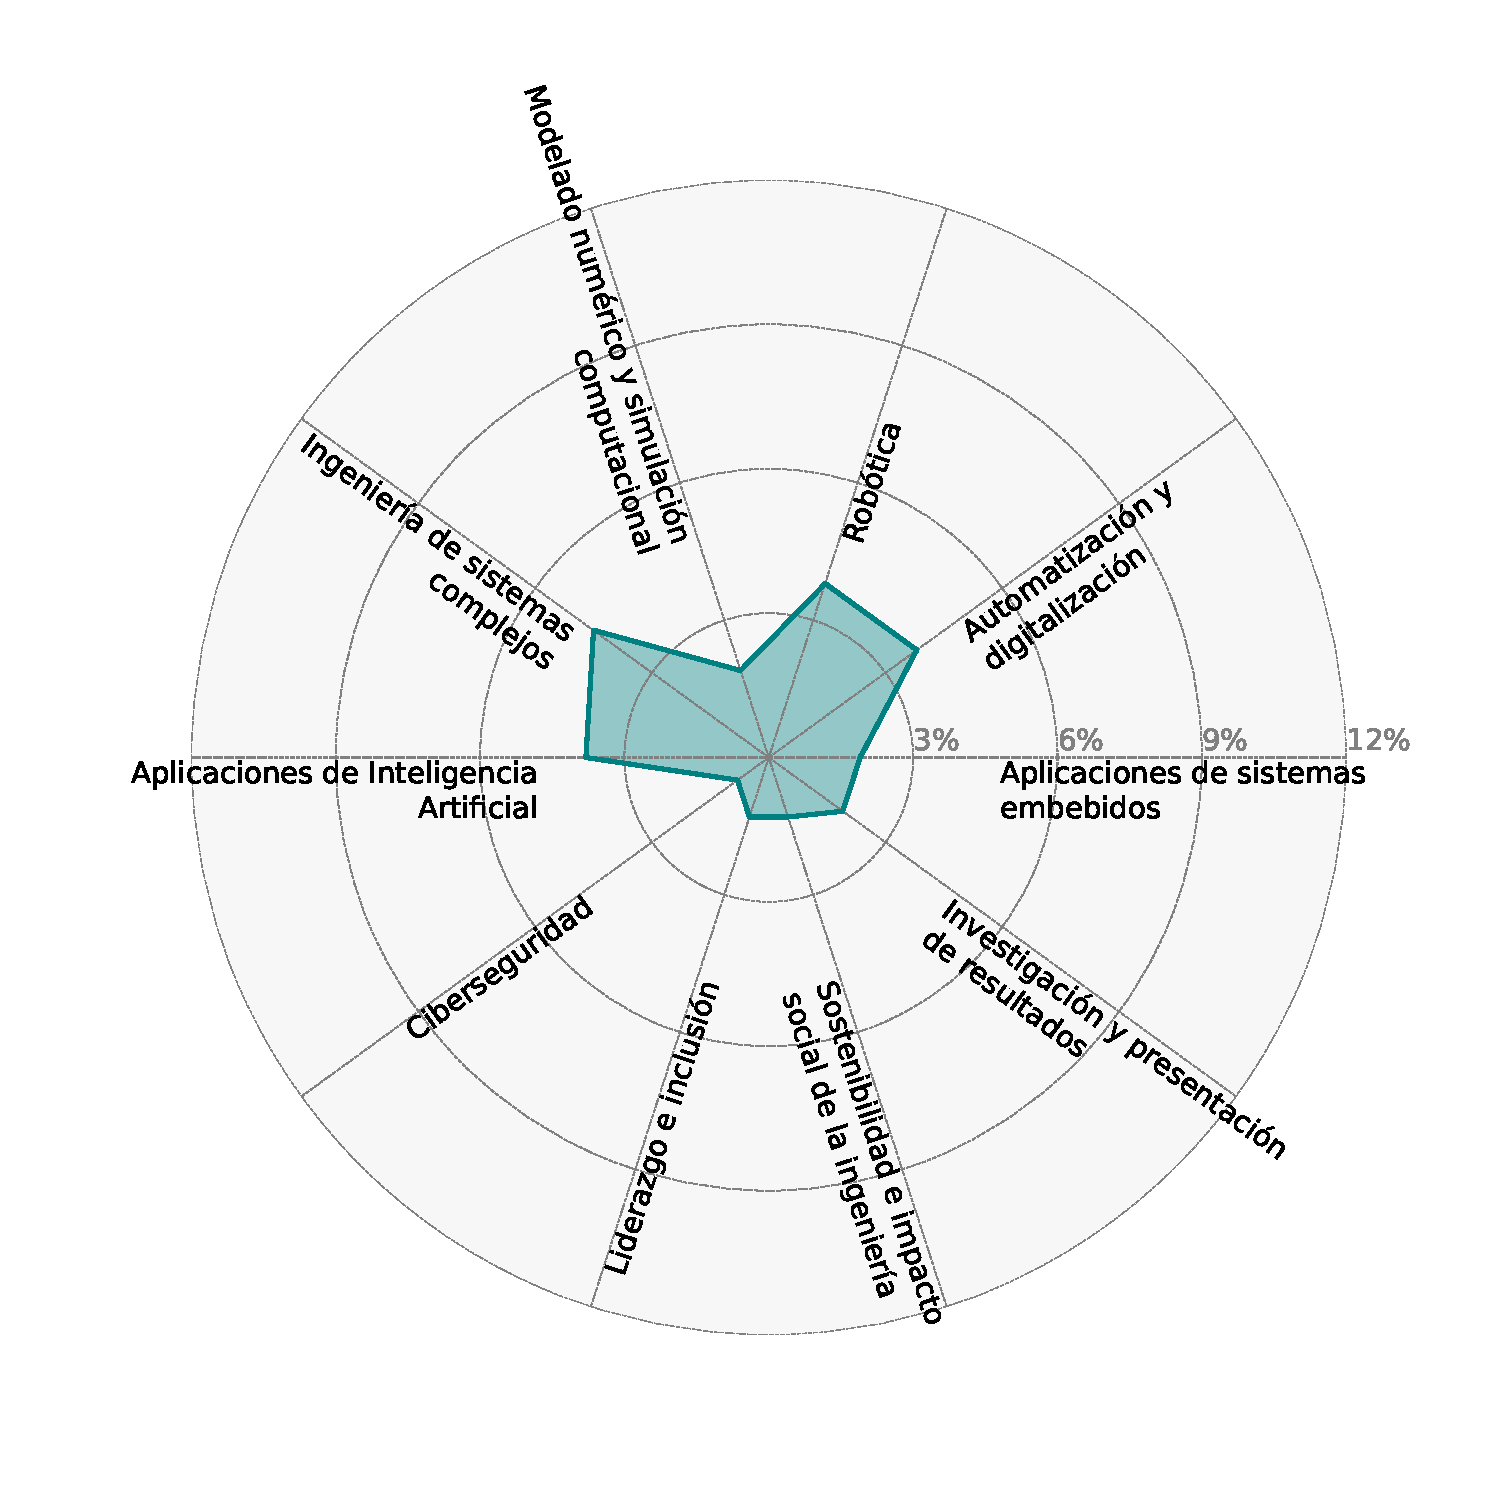
\includegraphics[width=.58\textwidth,height=.70\textheight,keepaspectratio]{generacion_graficos/salida/SCF.pdf}
\par\vspace{2mm}
{\centering\small Figura 7. Distribución porcentual de saberes para el énfasis en Sistemas ciberfísicos\par}
\end{figure}

\subsection*{Ejes curriculares}

Los ejes curriculares del programa han sido definidos tomando en consideración el PLANES 2021-2025, el Modelo Académico y pedagógico del TEC, las prácticas que han caracterizado las actividades de docencia de la Escuela Ingeniería Electromecánica y la naturaleza misma del objeto y sub-objetos de estudio.\par

\textit{Transdisciplinariedad}\par

Promueve no solo la integración de conocimientos provenientes de diversas disciplinas como la matemática, la física, la estadística, la ingeniería eléctrica, la mecánica y la automatización, sino también la construcción de un marco de conocimiento que trascienda las barreras tradicionales de las disciplinas.\par

El programa fomenta una interacción profunda entre estas áreas, facilitando una comprensión holística de los sistemas electromecánicos. Esto no solo implica el aprendizaje de planteamientos teóricos y metodológicos individuales, sino también la capacidad de fusionar y aplicar estos saberes en un contexto amplio, donde las soluciones a los problemas tecnológicos y sociales actuales requieren una visión integrada.\par

La transdisciplinariedad se expresa a través de un plan de estudios que aborda el diseño de sistemas complejos, la gestión de proyectos innovadores y sostenibles, y la capacidad para analizar datos y optimizar procesos mediante la automatización. Se favorece la creación de conocimiento y competencias que no se limiten a la frontera de cada disciplina, sino que aborden los desafíos desde múltiples perspectivas, facilitando la adaptación a las demandas cambiantes del sector industrial y tecnológico.\par

\textit{La Renovación Cognoscitiva}\par

En las sociedades de conocimiento, las universidades y otras instituciones de educación superior constituyen una de las principales fuentes de competitividad a nivel mundial, pues de ellas se espera que surja el nuevo conocimiento, el cual es el motor del desarrollo económico y del bienestar social.\par

En congruencia con lo anterior, el CONARE  estipula la necesidad de la renovación cognoscitiva, la cual se refiere a la generación de conocimiento que actualice los saberes que explican un determinado problema con el fin de contribuir al desarrollo de las sociedades, lo anterior a través de la investigación, inter, trans y multidisciplinaria.\par

Por su parte el TEC ha definido en su modelo académico que la investigación, como instrumento para la generación de conocimiento, debe potenciarse en mayor grado en los programas de pregrado y orientarse a la solución de problemas de sectores socioeconómicos específicos que generen beneficios para la sociedad costarricense.\par

En vista de lo anterior y del enfoque en investigación de este programa, la renovación cognoscitiva se adopta como eje curricular, entendida como la necesidad que durante el proceso formativo los estudiantes más allá que aprender conocimientos existentes, estén en capacidad para renovar esos conocimientos con aportaciones que han derivado de las investigaciones científicas aplicadas desarrolladas durante sus estudios.\par

\subsection*{Ejes transversales}

Los ejes transversales se constituyen en una práctica pedagógica que tiene por fin integrar una serie de elementos propios del currículo para lograr un aprendizaje significativo de los estudiantes. En ese sentido, esta carrera ha definido como ejes transversales de la Licenciatura en Ingeniería Electromecánica los siguientes:\par

\subsubsection*{Innovación y emprendedurismo}

Se promoverá lo indicado en el artículo 5 de la Ley Constitutiva del ITCR, que autoriza al TEC en el ofrecimiento bienes y servicios dentro de los campos de su actividad académica y le reconoce su plena capacidad jurídica para crear y participar en empresas, sociedades, empresas auxiliares académicas y tecnológicas. Adicionalmente, en el III Congreso Institucional del 2007 se aprobó que el Modelo Académico del Tecnológico de Costa Rica, en la sección 1.3, inciso c) que la Institución “potencia y consolida la creatividad, la innovación y el espíritu emprendedor fortaleciendo una actitud y capacidad de cuestionar, asumir riesgos, experimentar, investigar, crear y desarrollar. El espíritu emprendedor tiene una visión de cambio social y empresarial, de tal forma que se potencie el liderazgo de las personas en todas las estructuras de la sociedad costarricense.”\par

\subsubsection*{Vinculación con la industria}

Desarrollar relaciones de valor entre dependencias del TEC como fuera de ellas” (Instituto Tecnológico de Costa Rica, 2019). El programa promoverá las relaciones de cooperación con la industria, el Gobierno y otras universidades referentes de la electromecánica. Se fomentará la articulación de convenios y acuerdos para desarrollar iniciativas de docencia, investigación o extensión que beneficien y potencien estas relaciones.\par

\subsubsection*{Promoción de los ejes transversales del TEC}

Este programa ha adoptado el compromiso del Instituto Tecnológico de Costa Rica de velar por la persona, la igualdad, la excelencia y los principios democráticos, en virtud de ello se compromete con la promoción, en todas las actividades académicas y administrativas, que fueron definidos en el Modelo Académico, en el marco del III Congreso Institucional en el año 2007:\par

\begin{cuadrocafe}[EJT01]
El ser humano como principio y fin de la actividad institucional.
\end{cuadrocafe}

\begin{cuadrocafe}[EJT02]
El respeto a las diferencias de todas las personas.
\end{cuadrocafe}

\begin{cuadrocafe}[EJT03]
La necesidad de la formación integral de las personas.
\end{cuadrocafe}

\begin{cuadrocafe}[EJT04]
El acceso y permanencia en igualdad de oportunidades a las personas con potencial, sin distingos de etnia, religión, género, desarrollo psicoeducativo, necesidades especiales, condición socioeconómica y tendencia política.
\end{cuadrocafe}

\begin{cuadrocafe}[EJT05]
El fomento y fortalecimiento de la protección y sostenibilidad ambiental.
\end{cuadrocafe}

\begin{cuadrocafe}[EJT06]
La excelencia en sus diferentes actividades.
\end{cuadrocafe}

\begin{cuadrocafe}[EJT07]
La planificación como parte sustantiva e integral orientada al logro de la misión y visión institucionales.
\end{cuadrocafe}

\begin{cuadrocafe}[EJT08]
La rendición de cuentas, transparencia de la información y cultura de evaluación.
\end{cuadrocafe}

\begin{cuadrocafe}[EJT09]
El fomento y fortalecimiento de la cultura de paz.
\end{cuadrocafe}

Con la definición de estos ejes se busca orientar el análisis, la síntesis y la resolución de problemas de temas vinculados con la ingeniería electromecánica y la investigación básica y aplicada, promoviendo de este modo la integración entre la docencia y la investigación. Los ejes transversales del TEC se han codificado para facilitar el mapeo entre ejes transversales y rasgos que se realizará más adelante.\par

\subsubsection*{Promoción de los Objetivos de Desarrollo Sostenible de la ONU}

La inclusión de los Objetivos de Desarrollo Sostenible (ODS) como ejes transversales en la nueva carrera de Ingeniería Electromecánica garantiza que los estudiantes se alineen con las metas globales para el desarrollo sostenible. Esta integración les permite reconocer la importancia de su labor en un contexto global y su contribución hacia un futuro más equitativo y sostenible.\par

Los ingenieros tienen un papel fundamental en el diseño y desarrollo de tecnologías que impactan tanto a la sociedad como al medio ambiente. Al enfocar su formación en la sostenibilidad, los estudiantes podrán cultivar habilidades innovadoras para enfrentar los desafíos actuales y futuros de la ingeniería. Esto les brindará una ventaja competitiva en el mercado laboral, donde las empresas buscan cada vez más profesionales capaces de implementar soluciones sostenibles y eficientes.\par

En este nuevo programa, se han incorporado dos objetivos de desarrollo sostenible como ejes transversales de la formación académica:\par

\begin{cuadrocafe}[ODS07]
Objetivo 7. Energía asequible y no contaminante: la ingeniería electromecánica está intrínsecamente vinculada a la generación, distribución y uso eficiente de la energía. Fomentar este objetivo ayudará a los estudiantes a desarrollar conciencia sobre el diseño y la selección de tecnologías energéticas sostenibles y limpias, fundamentales para combatir el cambio climático y reducir la dependencia de combustibles fósiles.
\end{cuadrocafe}

\begin{cuadrocafe}[ODS09]
Objetivo 9. Industria, innovación e infraestructura: Este objetivo resalta la importancia de construir infraestructuras resilientes y promover una industrialización sostenible. La formación de ingenieros electromecánicos en este ámbito estimulará la innovación en el diseño de procesos industriales y mejorará la eficiencia en el uso de recursos, contribuyendo al desarrollo económico sin comprometer el medio ambiente.
\end{cuadrocafe}

Integrar estos objetivos en el programa de Ingeniería Electromecánica no solo enriquecerá la formación académica de los estudiantes, sino que también los preparará para desempeñarse en un mundo que demanda un enfoque más sostenible en la ingeniería y la tecnología. Esto ayudará a formar profesionales comprometidos con el desarrollo sostenible y la mejora de la calidad de vida. Los ODS se han codificado para facilitar el mapeo entre ejes transversales y rasgos que se realizará más adelante.\par

\subsubsection*{Promoción de los Descriptores del Marco de Cualificaciones para la Educación Superior Centroamericana (MCESCA)}

El Marco de Cualificaciones para la Educación Superior Centroamericana establece los resultados de aprendizaje esperados para un grado de licenciatura. El nuevo programa de la carrera de Ingeniería Electromecánica se compromete con el cumplimiento de estos aprendizajes esperados. De esta manera, la nueva carrera se compromete con que el estudiante graduado de este programa podrá:\par

\begin{cuadrocafe}[MCA01]
Comprender en forma crítica el cuerpo conceptual, metodológico, procedimental y normativo, que le permitirá el ejercicio de su profesión en el contexto nacional e internacional.
\end{cuadrocafe}

\begin{cuadrocafe}[MCA02]
Identificar oportunidades y riesgos para la innovación y adaptación de conocimientos y tecnologías para resolver problemas.
\end{cuadrocafe}

\begin{cuadrocafe}[MCA03]
Demostrar pensamiento crítico, actitud investigativa y rigor analítico en el planteamiento y la resolución de problemas complejos.
\end{cuadrocafe}

\begin{cuadrocafe}[MCA04]
Aplicar los conocimientos de su disciplina en la elaboración, fundamentación y defensa de argumentos para prevenir y resolver problemas complejos en su campo profesional, identificando y aplicando innovaciones.
\end{cuadrocafe}

\begin{cuadrocafe}[MCA05]
Proponer e implementar nuevos procedimientos y metodologías aplicables a la solución de problemas complejos y mejora de su campo profesional.
\end{cuadrocafe}

\begin{cuadrocafe}[MCA06]
Tomar decisiones profesionales con base en fundamentos teóricos, datos e información pertinente, válida y confiable.
\end{cuadrocafe}

\begin{cuadrocafe}[MCA07]
Identificar sus necesidades de actualización, capacitación y formación, durante su proceso formativo y en el ejercicio profesional, y busca los medios para cubrirlas.
\end{cuadrocafe}

\begin{cuadrocafe}[MCA08]
Comunicar información de su campo profesional de manera asertiva, clara, rigurosa y precisa, tanto en inglés como en español.
\end{cuadrocafe}

\begin{cuadrocafe}[MCA09]
Utilizar el inglés con el dominio requerido para el ejercicio de su profesión.
\end{cuadrocafe}

\begin{cuadrocafe}[MCA10]
Liderar y colaborar proactivamente en equipos de trabajo y comunidades profesionales para el logro de objetivos y mejoramiento de la calidad de vida.
\end{cuadrocafe}

Los Descriptores de MCESCA se han codificado para facilitar el mapeo entre ejes transversales y rasgos que se realizará más adelante.\par

\subsection*{Principios metodológicos}

Los principios metodológicos y evaluativos que definen los términos en que se enseñará, se aprenderá y se evaluará, para que el estudiante adquiera el perfil académico profesional ideal, se presentan en este apartado, los cuales son coherentes con los lineamientos definidos en el Modelo Académico del TEC y particularmente su modelo pedagógico el cual fue aprobado en el IV Congreso Institucional en el año 2019.\par

\subsubsection*{Fundamentación teórica del modelo metodológico y evaluativo}

El modelo de este programa se sustenta en el Modelo Pedagógico del TEC , aprobado en el 2019 en el IV Congreso Institucional, propone teóricamente dos epistemologías: el constructivismo y la corriente sistémico-compleja. Ello justificado por ser las que mejor se adaptan a la era del conocimiento y a la naturaleza tecnológica-científica del Instituto Tecnológico de Costa Rica y de este programa de licenciatura. Los principios teórico-pedagógicos sustentados en bases ontológicas, epistemológicas y paradigmáticas sobre las cuales se fundamenta este Modelo Pedagógico, se oponen a concepciones educativas tradicionalistas de índole mecánico (automático), repetitivo del aprendizaje, y al rol pasivo del estudiante muy característico de la corriente conductista. Por lo tanto, los principios epistémicos del modelo propician la transformación del proceso educativo al proponer un aprendizaje significativo, humanista, competente, pedagógico y autónomo. En general, el Modelo Pedagógico del TEC:\par

\textit{...tiene como finalidad desarrollar en el estudiantado los procesos del pensamiento, la construcción del conocimiento, el crecimiento personal, social, intelectual, actitudinal, científico y axiológico, de forma que contribuyan con la evolución de la sociedad, mediante un ejercicio profesional competente. Infiere de sus raíces epistemológicas una enseñanza dinámica, responsable y multidireccional en la que interactúan responsablemente el equipo docente, la comunidad estudiantil, lo curricular y el rol institucional, en relaciones sinérgicas en procura de favorecer un proceso formativo inteligente, abierto, reflexivo, aplicable, competitivo y motivante.}\par

Por esta razón, se establece el concepto de investigación práctica aplicada (que se explica en detalle más adelante), como la estrategia didáctica principal por medio de la cual los estudiantes en forma paralela a los cursos tendrán espacios significativos, activos, participativos y dinámicos para el aprendizaje y la investigación. Esto se llevará a cabo por medio del desarrollo de tipos de investigaciones aplicadas como: elaboración análisis de alternativas, análisis de brechas, análisis comparativos, formulación de casos, implementación de buenas prácticas de industria, construcción de prototipos o simulaciones, metodologías de diseño, análisis de riesgos, entre otros. Todos ellos con una perspectiva de inmersión laboral y donde esta estrategia metodológica es clara en resaltar el rol del estudiante como centro del proceso de aprendizaje.  Además, sugiere claramente que la enseñanza es relevante en el tanto el profesor asume su papel como orientador del proceso de aprendizaje. En consecuencia, este programa tiene como pilar la investigación en el aula (presencial o telepresencial) y por tanto el proceso de aprendizaje y enseñanza será un espacio de interacción de la experiencia del estudiante en el ejercicio académico de construir nuevo conocimiento.\par

El Programa adopta esta corriente de pensamiento asumiendo el hecho que el proceso formativo que implica este programa dará la oportunidad al estudiante de que tome conciencia de sus experiencias y las evalúe para encontrar una solución a la luz del conocimiento existente.\par

\subsubsection*{Rol y responsabilidad del profesor}

Bajo la teoría andragógica del aprendizaje el profesor se aparta de la tradicional figura autoritaria para convertirse en un facilitador que colaborará con los entendimientos de las experiencias de los estudiantes, esto implica que el profesor también aprende de sus estudiantes; sus conocimientos y los de los estudiantes son intercambiables .\par

El rol del profesor, según el Modelo Académico del TEC será promover en los estudiantes su capacidad de aprender a aprender. En virtud de lo anterior, el profesor de este programa de licenciatura asumirá un rol en el cual:\par

\begin{enumerate}
\item Crea un clima de confianza y adopta una actitud de humildad para aprender con los estudiantes en el proceso de evaluar las experiencias, promoviendo la interacción social como mecanismo fundamental para el desarrollo de la cognición.
\item Desarrolla interés en el estudiante por la investigación con ejemplos prácticos y significativos de sus propias investigaciones y experiencias.
\item Se convierte en un facilitador en los procesos de formación de los estudiantes, más que imponer autoritariamente sus conocimientos.
\item Se convierte en un asesor cuyo propósito básico es que el estudiante aprenda a aprender.
\item Reconoce que el grupo de estudiantes puede estar compuesto por personas muy distintas –edad, motivación, experiencia- y en consecuencia aprenden por métodos y en tiempos diferentes, se trata de una enseñanza centrada en la persona.
\item Dinamiza las clases a través de la articulación de las experiencias que aportan los estudiantes para que en su conjunto den sentido y aplicación práctica a los temas de los cursos.
\item Genera espacios para que los estudiantes analicen y cuestionen los temas del curso.
\item Promueve el pensamiento crítico hacia el conocimiento existente, a través de la discusión de paradigmas opuestos a las temáticas del curso.
\item Promueve actividades en las que los estudiantes aprendan de los errores que cometen.
\item Promueve la formación de competencias intelectuales, éticas, sociales y afectivas.
\item Motiva al estudiante en el aprendizaje y dominio del arte de la investigación, principalmente la aplicada a los contextos de la industria, gobierno y sociedad.
\end{enumerate}
\subsubsection*{Rol y responsabilidad del estudiante}

Con lo indicado en el Modelo Pedagógico del TEC, la concepción que esta licenciatura tiene del estudiante implica que éste:\par

\begin{enumerate}
\item Demuestra un desarrollo progresivo en su capacidad para autodirigirse e independizarse del profesor en los procesos de aprendizaje. Es un estudiante con autonomía y automotivación que muestra compromiso activo de ser responsable con su propio aprendizaje.
\item Participa activamente en la clase más que como espectador pasivo, a través de las experiencias que ha tenido y que se relacionan con los contenidos del curso.
\item Reflexiona, elabora ideas y emite juicios en relación con los temas del curso.
\item Demuestra apertura al pensamiento crítico y cuestiona las bases del conocimiento. Es capaz de evaluar las implicaciones de las acciones u omisiones de su desempeño como miembro de la universidad y la sociedad.
\item Investiga y sintetiza sobre los diversos planteamientos teóricos que existen en relación con el tema que se trata en cada curso.
\item Ejecuta trabajos de investigación práctica aplicada al campo como parte de las investigaciones que deberá desarrollar durante su paso por el Programa.
\item Ejecuta con rigurosidad científica y calidad las asignaciones que cada curso le demanda.
\item Más que preocuparse por memorizar datos aislados, se ocupa de entender el valor subyacente de las ideas o postulados de un tema en particular.
\item Comprende que el éxito académico y profesional tiene como condición previa una base de conocimientos bien estructurada.
\end{enumerate}
\subsubsection*{Rol y responsabilidad del personal de apoyo}

El personal de apoyo del Programa se encargará de brindar el soporte administrativo a los estudiantes y a los profesores, esto implica que:\par

\begin{enumerate}
\item Muestre empatía por las necesidades de los estudiantes, de modo que se pueda ofrecer una solución que resuelva los problemas, en los que tiene competencia para actuar.
\item Atienda oportunamente a las solicitudes de colaboración de parte de los profesores.
\item Coordina la dotación de los recursos didácticos que serán requeridos por el profesor para el desarrollo de las clases.
\item Realiza los procedimientos administrativos que son necesarios para el desarrollo de las actividades académicas.
\item Ofrece oportunidades de integración de los estudiantes con las demás actividades de investigación, docencia y extensión de la Institución.
\item Establece comunicación estrecha con los estudiantes actuales y egresados del programa.
\end{enumerate}
\subsubsection*{Relación profesor-estudiante-personal de apoyo}

La relación de profesor-estudiante se fundará sobre los valores del respeto, la honestidad, la solidaridad, la transparencia y la empatía, los cuales permitirán crear espacios para el aprendizaje mutuo, por medio de la construcción del conocimiento sobre la base del ya existente (experiencias de profesores y estudiantes).\par

En esta relación el profesor abandona la posición de profeta de la verdad o dictador del conocimiento para convertirse en la contraparte del estudiante en el debate y la crítica sobre los distintos postulados teóricos que se tratan en los cursos.\par

Asimismo, el personal de apoyo intervendrá en esta relación en procura de la creación de condiciones y los espacios favorables para el aprendizaje y construcción de conocimiento de estudiantes y profesores.\par

\subsubsection*{Método de enseñanza del profesor}

Con fundamento en el estado del conocimiento planteado en el modelo pedagógico del TEC, los métodos de enseñanza que utilice el profesor deben ser experimentales y en menor medida los de transmisión. Esto quiere decir que el aprendizaje del estudiante resultará de la aplicación de los temas a sus experiencias, ya que para despertar su interés por aprender algo antes necesitan saber por qué es importante aprenderlo y qué problema de la vida real les ayuda a solucionar , además deberán ser heurísticos, es decir, orientados al descubrimiento. En apego a Knowles  se propone que el ejercicio de estos métodos de enseñanza deberá permitir al profesor lograr lo siguiente:\par

\begin{enumerate}
\item Hacer del estudiante un sujeto activo, que se involucre y participe en la solución de los desafíos que plantea la actividad.
\item La reiteración activa de la acción investigativa con el objetivo de que el estudiante adquiere los aprendizajes y desarrolle las habilidades que se desprenden del nuevo conocimiento.
\item La generalización y la discriminación, el método generará en el estudiante la capacidad para discriminar en qué situaciones conviene la aplicación de una determinada solución y en qué otras no.
\end{enumerate}
\subsubsection*{Desarrollo de habilidades en la formación profesional}

El desarrollo de competencias profesionales, es fundamental para un desarrollo exitoso, combinando conocimientos, habilidades, valores y actitudes en el contexto profesional, de ahí que, en dicho desarrollo, debe estar presente en forma transversal en el programa de estudio, de manera que la formación no solo  supla las necesidades de conocimiento técnico, sino también impacte de forma positiva en  el desarrollo de nuevas habilidades socioafectivas, las cuales son muy útiles en el ejercicio de la profesión. Es así como el fundamento de la ingeniería electromecánica considera una formación integral que incluya aspectos propios de su quehacer disciplinario, fortalecido con realización de prácticas de laboratorio y la promoción de habilidades y destrezas, que suponen un mejor desempeño laboral.\par

\subsubsection*{Metodología y evaluación}

Dado que la metodología de enseñanza pretende dotar o construir conocimientos, desarrollo de habilidades, aplicación de  técnicas, promoción de habilidades  de convivencia o socioafectivas e interacción en un entorno dinámico y cambiante, la evaluación del aprendizaje debe estar alineada y consecuente, promoviendo a través de diversas herramientas y estrategias evaluativas,  la verificación del conocimiento y desarrollo de habilidades en el marco de una ingeniería electromecánica, incluyendo rubros como el  desarrollo de proyectos, uso de  herramientas de simulación, programación, análisis de casos, análisis de datos,  preparación de informes técnicos, entre otros.\par

En el Reglamento del Régimen Enseñanza-Aprendizaje y el Estatuto Orgánico del Instituto Tecnológico de Costa Rica, se mencionan tres formas de evaluación principales: diagnóstica, formativa y sumativa. A continuación, se resumen estas evaluaciones y su relación con la evaluación auténtica y el enfoque multimetodológico del :\par

\paragraph{Formas de Evaluación:}

\begin{itemize}
\item Evaluación Diagnóstica: Se utiliza al inicio de un curso o unidad de aprendizaje para identificar el nivel de conocimientos previos y habilidades de los estudiantes. Su propósito es ayudar al docente a ajustar los contenidos y metodologías según las necesidades del grupo.
\item Evaluación Formativa: Esta evaluación se lleva a cabo durante todo el proceso de enseñanza-aprendizaje. Tiene un carácter continuo y está orientada a la mejora del aprendizaje a través de la retroalimentación constante, permitiendo a los estudiantes y docentes ajustar su enfoque. Ayuda a identificar dificultades y éxitos, promoviendo un aprendizaje más efectivo.
\item Evaluación Sumativa: Se realiza al final de un ciclo o curso para valorar de manera global los aprendizajes alcanzados. Se utiliza generalmente para asignar calificaciones finales y determinar el grado de cumplimiento de los objetivos de aprendizaje.
\end{itemize}
\paragraph{Relación con la Evaluación Auténtica:}

La evaluación auténtica se enfoca en la aplicación de conocimientos y habilidades en contextos reales o simulados. Está alineada principalmente con la evaluación formativa, ya que promueve la resolución de problemas reales a lo largo del curso, en lugar de centrarse únicamente en exámenes tradicionales como la evaluación sumativa. Este tipo de evaluación permite a los estudiantes demostrar sus competencias en situaciones prácticas y relevantes para su campo profesional.\par

\paragraph{Relación con el Enfoque Multimetodológico:}

El enfoque multimetodológico combina diferentes métodos y estrategias pedagógicas, adaptando la enseñanza a diversas formas de aprendizaje. La evaluación formativa es clave en este enfoque, ya que permite el uso de múltiples métodos para medir el progreso, como observaciones, proyectos, y presentaciones. La evaluación diagnóstica ayuda a elegir los métodos adecuados al perfil del estudiante, y la evaluación sumativa verifica el éxito del enfoque integrado a través de exámenes finales o trabajos de fin de curso.\par

Este enfoque facilita una evaluación integral que se ajusta a las necesidades individuales y colectivas de los estudiantes, promoviendo un aprendizaje más completo y auténtico.\par

Finalmente, es importante indicar que todos estos elementos metodológicos, evaluativos y pedagógicos se verán reflejados en el desarrollo didáctico de cada uno de los cursos de la carrera, donde existirá elementos o rasgos de estos principios que hacen visible su hilaridad y coherencia a través de todo el proceso de enseñanza y aprendizaje.\par

Propósitos\par

\subsection*{Propósitos de la Escuela}

\subsubsection*{Misión}

Promover el desarrollo integral de la sociedad por medio de la investigación, la extensión y la formación del talento humano de excelencia, basados en pilares éticos, humanísticos y ambientales, en busca de la competitividad y calidad en el ámbito nacional e internacional.\par

\subsubsection*{Visión}

Será un ente líder en su campo, capaz de interactuar con otros sectores a nivel nacional e internacional, en el intercambio y creación de conocimiento impulsando el desarrollo social y económico. Estará al servicio de la sociedad, industria y comunidad científica, por medio de la docencia, la investigación, la extensión y la formación de profesionales innovadores, emprendedores y comprometidos con la justicia social, respeto por los derechos humanos y el ambiente.\par

\subsection*{Propósitos del programa}

\subsubsection*{Misión}

Formar profesionales en Ingeniería Electromecánica con un perfil académico-profesional de calidad, competitivo a nivel nacional e internacional, en concordancia con las normas éticas, humanistas y ambientales.\par

\subsubsection*{Visión}

Será una carrera universitaria actual, de calidad y con vocación de mejora continua, reconocida a nivel nacional e internacional por brindar una formación de excelencia a las personas egresadas, habilitándoles para participar activamente en el desarrollo del país.\par

\section*{Perfil académico-profesional del programa y sus énfasis}

\subsection*{Perfil del tronco común y salida lateral de bachillerato}

Al finalizar el tronco común del programa de Licenciatura en Ingeniería Electromecánica o tomar la salida lateral de Bachillerato en Ingeniería Electromecánica la persona estudiante se ha desarrollado y formado en el siguiente perfil académico-profesional\par

\subsubsection*{Ciencias básicas}

Comprende el conocimiento fundamental en matemáticas, física y química, esenciales para el desarrollo de habilidades analíticas y la comprensión de los principios que sustentan la ingeniería.\par

Rasgos del perfil:\par

\begin{cuadroazul}[CIB01]
Conocer y aplicar los fundamentos de la matemática, la física, y la química necesarios para el análisis, diseño y desarrollo de sistemas electromecánicos.
\end{cuadroazul}

\subsubsection*{Formación profesional y habilidades Interpersonales}

Abarca las competencias éticas, sociales y laborales, así como el liderazgo, emprendimiento y administración de proyectos.\par

Rasgos del perfil:\par

\begin{cuadroazul}[FPH01]
Actuar con integridad y responsabilidad social en el ejercicio de la ingeniería, fomentando una comunicación efectiva y una actitud colaborativa en equipos de trabajo, y promoviendo una cultura de salud, seguridad y bienestar en el entorno laboral.
\end{cuadroazul}

\begin{cuadroazul}[FPH02]
Identificar oportunidades de negocio en el ámbito de la ingeniería, desarrollando soluciones innovadoras y sostenibles que agreguen valor a la sociedad.
\end{cuadroazul}

\begin{cuadroazul}[FPH03]
Administrar eficientemente proyectos, garantizando el cumplimiento de objetivos técnicos, financieros y de tiempo.
\end{cuadroazul}

\subsubsection*{Comunicación y dibujo}

Comprende lo relacionado con la comunicación de ideas de manera efectiva, tanto oralmente como por escrito, y el uso del dibujo para la representación gráfica en la ingeniería.\par

Rasgos del perfil:\par

\begin{cuadroazul}[CYD01]
Estructurar sus ideas de manera clara y transmitirlas de forma oral, escrita o mediante dibujos de ingeniería, tanto en español como en inglés.
\end{cuadroazul}

\subsubsection*{Ingeniería eléctrica y electrónica}

Abarca los circuitos, máquinas eléctricas y electrónica, áreas fundamentales para la operación y diseño de sistemas electromecánicos.\par

Rasgos del perfil:\par

\begin{cuadroazul}[IEE01]
Conocer y aplicar los principios de los circuitos eléctricos y la electrónica, y analizar su funcionamiento en las diversas aplicaciones en ingeniería electromecánica.
\end{cuadroazul}

\begin{cuadroazul}[IEE02]
Evaluar el comportamiento de las máquinas eléctricas bajo diversas condiciones de operación, así como analizar su diseño y aplicaciones.
\end{cuadroazul}

\begin{cuadroazul}[IEE03]
Implementar sistemas de instrumentación para la medición de variables físicas en sistemas electromecánicos.
\end{cuadroazul}

\subsubsection*{Ingeniería mecánica y de materiales}

Comprende el estudio de materiales y su comportamiento, así como los principios de la mecánica, termodinámica y manufactura aplicados en el diseño y análisis de sistemas mecánicos.\par

Rasgos del perfil:\par

\begin{cuadroazul}[IMM01]
Evaluar las características de los materiales y seleccionar los procesos de manufactura adecuados para el desarrollo y la producción de sistemas electromecánicos.
\end{cuadroazul}

\begin{cuadroazul}[IMM02]
Aplicar los principios de la mecánica de sólidos y fluidos, termodinámica y transferencia de calor para analizar el comportamiento de los sistemas electromecánicos.
\end{cuadroazul}

\subsubsection*{Automática}

Incluye la programación, el control y la automatización de sistemas, incluyendo modelado y simulación, lo que permite optimizar procesos y mejorar la eficiencia de los sistemas electromecánicos.\par

Rasgos del perfil:\par

\begin{cuadroazul}[AUT01]
Desarrollar soluciones de software para el control y procesamiento de datos en sistemas electromecánicos.
\end{cuadroazul}

\begin{cuadroazul}[AUT02]
Desarrollar soluciones de hardware usando microcontroladores para el control y procesamiento de datos en sistemas electromecánicos.
\end{cuadroazul}

\begin{cuadroazul}[AUT03]
Diseñar e implementar sistemas de control y automatización en sistemas electromecánicos integrando modelado y simulación.
\end{cuadroazul}

\subsubsection*{Análisis de datos}

Se centra en el uso de estadísticas, metrología y diseño de experimentos para la recopilación, análisis e interpretación de datos, cruciales para la toma de decisiones en el ámbito de la ingeniería.\par

Rasgos del perfil:\par

\begin{cuadroazul}[ADD01]
Aplicar herramientas estadísticas, evaluar datos con rigor científico, y garantizar la confiabilidad, disponibilidad, mantenibilidad y seguridad en sistemas electromecánicos.
\end{cuadroazul}

\begin{cuadroazul}[ADD02]
Aplicar principios de metrología para medir variables físicas en sistemas electromecánicos
\end{cuadroazul}

\subsection*{Mapeo de ejes transversales en rasgos de perfil para el tronco común y salida lateral de bachillerato}

\begin{center}
\scriptsize
\arrayrulecolor{azulTEC}
\begin{adjustbox}{max width=\textwidth,max totalheight=.82\textheight}
\begin{tabular}{|l|c|c|c|c|c|c|c|c|c|c|c|c|c|c|c|c|c|c|c|c|c|}
\hline
\rowcolor{azulTEC}
\textcolor{white}{\textbf{\rule{0pt}{1.35cm}rasgos / ejes}} & \textcolor{white}{\textbf{\rotatebox{90}{\strut EJT01}}} & \textcolor{white}{\textbf{\rotatebox{90}{\strut EJT02}}} & \textcolor{white}{\textbf{\rotatebox{90}{\strut EJT03}}} & \textcolor{white}{\textbf{\rotatebox{90}{\strut EJT04}}} & \textcolor{white}{\textbf{\rotatebox{90}{\strut EJT05}}} & \textcolor{white}{\textbf{\rotatebox{90}{\strut EJT06}}} & \textcolor{white}{\textbf{\rotatebox{90}{\strut EJT07}}} & \textcolor{white}{\textbf{\rotatebox{90}{\strut EJT08}}} & \textcolor{white}{\textbf{\rotatebox{90}{\strut EJT09}}} & \textcolor{white}{\textbf{\rotatebox{90}{\strut MCA01}}} & \textcolor{white}{\textbf{\rotatebox{90}{\strut MCA02}}} & \textcolor{white}{\textbf{\rotatebox{90}{\strut MCA03}}} & \textcolor{white}{\textbf{\rotatebox{90}{\strut MCA04}}} & \textcolor{white}{\textbf{\rotatebox{90}{\strut MCA05}}} & \textcolor{white}{\textbf{\rotatebox{90}{\strut MCA06}}} & \textcolor{white}{\textbf{\rotatebox{90}{\strut MCA07}}} & \textcolor{white}{\textbf{\rotatebox{90}{\strut MCA08}}} & \textcolor{white}{\textbf{\rotatebox{90}{\strut MCA09}}} & \textcolor{white}{\textbf{\rotatebox{90}{\strut MCA10}}} & \textcolor{white}{\textbf{\rotatebox{90}{\strut ODS07}}} & \textcolor{white}{\textbf{\rotatebox{90}{\strut ODS09}}} \\ \hline
\rowcolor{azulClaro}
\textcolor{azulTEC}{\textbf{CIB01}} & \textbf{ } & \textbf{ } & \textbf{ } & \textbf{ } & \textbf{ } & \textbf{ } & \textbf{ } & \textbf{ } & \textbf{ } & \textbf{X} & \textbf{ } & \textbf{ } & \textbf{ } & \textbf{ } & \textbf{ } & \textbf{ } & \textbf{ } & \textbf{ } & \textbf{ } & \textbf{ } & \textbf{ } \\ \hline
\rowcolor{azulClaro}
\textcolor{azulTEC}{\textbf{FPH01}} & \textbf{X} & \textbf{ } & \textbf{X} & \textbf{ } & \textbf{ } & \textbf{ } & \textbf{ } & \textbf{ } & \textbf{X} & \textbf{ } & \textbf{ } & \textbf{ } & \textbf{ } & \textbf{ } & \textbf{ } & \textbf{X} & \textbf{ } & \textbf{ } & \textbf{ } & \textbf{ } & \textbf{ } \\ \hline
\rowcolor{azulClaro}
\textcolor{azulTEC}{\textbf{FPH02}} & \textbf{ } & \textbf{ } & \textbf{ } & \textbf{ } & \textbf{ } & \textbf{X} & \textbf{ } & \textbf{ } & \textbf{ } & \textbf{ } & \textbf{X} & \textbf{ } & \textbf{ } & \textbf{ } & \textbf{ } & \textbf{ } & \textbf{ } & \textbf{ } & \textbf{ } & \textbf{ } & \textbf{X} \\ \hline
\rowcolor{azulClaro}
\textcolor{azulTEC}{\textbf{FPH03}} & \textbf{ } & \textbf{ } & \textbf{ } & \textbf{ } & \textbf{ } & \textbf{ } & \textbf{X} & \textbf{X} & \textbf{ } & \textbf{ } & \textbf{ } & \textbf{X} & \textbf{ } & \textbf{ } & \textbf{ } & \textbf{ } & \textbf{ } & \textbf{ } & \textbf{X} & \textbf{ } & \textbf{ } \\ \hline
\rowcolor{azulClaro}
\textcolor{azulTEC}{\textbf{CYD01}} & \textbf{ } & \textbf{ } & \textbf{X} & \textbf{ } & \textbf{ } & \textbf{ } & \textbf{ } & \textbf{ } & \textbf{ } & \textbf{ } & \textbf{ } & \textbf{ } & \textbf{ } & \textbf{ } & \textbf{ } & \textbf{ } & \textbf{X} & \textbf{X} & \textbf{ } & \textbf{ } & \textbf{ } \\ \hline
\rowcolor{azulClaro}
\textcolor{azulTEC}{\textbf{IEE01}} & \textbf{ } & \textbf{ } & \textbf{ } & \textbf{ } & \textbf{ } & \textbf{ } & \textbf{ } & \textbf{ } & \textbf{ } & \textbf{X} & \textbf{ } & \textbf{ } & \textbf{ } & \textbf{ } & \textbf{ } & \textbf{ } & \textbf{ } & \textbf{ } & \textbf{ } & \textbf{ } & \textbf{ } \\ \hline
\rowcolor{azulClaro}
\textcolor{azulTEC}{\textbf{IEE02}} & \textbf{ } & \textbf{ } & \textbf{ } & \textbf{ } & \textbf{ } & \textbf{ } & \textbf{ } & \textbf{ } & \textbf{ } & \textbf{X} & \textbf{ } & \textbf{ } & \textbf{ } & \textbf{ } & \textbf{ } & \textbf{ } & \textbf{ } & \textbf{ } & \textbf{ } & \textbf{ } & \textbf{ } \\ \hline
\rowcolor{azulClaro}
\textcolor{azulTEC}{\textbf{IEE03}} & \textbf{ } & \textbf{ } & \textbf{ } & \textbf{ } & \textbf{ } & \textbf{ } & \textbf{ } & \textbf{ } & \textbf{ } & \textbf{X} & \textbf{ } & \textbf{ } & \textbf{ } & \textbf{ } & \textbf{ } & \textbf{ } & \textbf{ } & \textbf{ } & \textbf{ } & \textbf{ } & \textbf{ } \\ \hline
\rowcolor{azulClaro}
\textcolor{azulTEC}{\textbf{IMM01}} & \textbf{ } & \textbf{ } & \textbf{ } & \textbf{ } & \textbf{ } & \textbf{ } & \textbf{ } & \textbf{ } & \textbf{ } & \textbf{X} & \textbf{ } & \textbf{ } & \textbf{ } & \textbf{ } & \textbf{ } & \textbf{ } & \textbf{ } & \textbf{ } & \textbf{ } & \textbf{ } & \textbf{ } \\ \hline
\rowcolor{azulClaro}
\textcolor{azulTEC}{\textbf{IMM02}} & \textbf{ } & \textbf{ } & \textbf{ } & \textbf{ } & \textbf{ } & \textbf{ } & \textbf{ } & \textbf{ } & \textbf{ } & \textbf{X} & \textbf{ } & \textbf{ } & \textbf{ } & \textbf{ } & \textbf{ } & \textbf{ } & \textbf{ } & \textbf{ } & \textbf{ } & \textbf{ } & \textbf{ } \\ \hline
\rowcolor{azulClaro}
\textcolor{azulTEC}{\textbf{AUT01}} & \textbf{ } & \textbf{ } & \textbf{ } & \textbf{ } & \textbf{ } & \textbf{ } & \textbf{ } & \textbf{ } & \textbf{ } & \textbf{X} & \textbf{ } & \textbf{ } & \textbf{ } & \textbf{ } & \textbf{ } & \textbf{ } & \textbf{ } & \textbf{ } & \textbf{ } & \textbf{ } & \textbf{ } \\ \hline
\rowcolor{azulClaro}
\textcolor{azulTEC}{\textbf{AUT02}} & \textbf{ } & \textbf{ } & \textbf{ } & \textbf{ } & \textbf{ } & \textbf{ } & \textbf{ } & \textbf{ } & \textbf{ } & \textbf{X} & \textbf{ } & \textbf{ } & \textbf{ } & \textbf{ } & \textbf{ } & \textbf{ } & \textbf{ } & \textbf{ } & \textbf{ } & \textbf{ } & \textbf{ } \\ \hline
\rowcolor{azulClaro}
\textcolor{azulTEC}{\textbf{AUT03}} & \textbf{ } & \textbf{ } & \textbf{ } & \textbf{ } & \textbf{ } & \textbf{ } & \textbf{ } & \textbf{ } & \textbf{ } & \textbf{X} & \textbf{ } & \textbf{ } & \textbf{ } & \textbf{ } & \textbf{ } & \textbf{ } & \textbf{ } & \textbf{ } & \textbf{ } & \textbf{ } & \textbf{ } \\ \hline
\rowcolor{azulClaro}
\textcolor{azulTEC}{\textbf{ADD01}} & \textbf{ } & \textbf{ } & \textbf{ } & \textbf{ } & \textbf{ } & \textbf{ } & \textbf{ } & \textbf{ } & \textbf{ } & \textbf{X} & \textbf{ } & \textbf{ } & \textbf{ } & \textbf{ } & \textbf{ } & \textbf{ } & \textbf{ } & \textbf{ } & \textbf{ } & \textbf{ } & \textbf{ } \\ \hline
\rowcolor{azulClaro}
\textcolor{azulTEC}{\textbf{ADD02}} & \textbf{ } & \textbf{ } & \textbf{ } & \textbf{ } & \textbf{ } & \textbf{ } & \textbf{ } & \textbf{ } & \textbf{ } & \textbf{X} & \textbf{ } & \textbf{ } & \textbf{ } & \textbf{ } & \textbf{ } & \textbf{ } & \textbf{ } & \textbf{ } & \textbf{ } & \textbf{ } & \textbf{ } \\ \hline
\end{tabular}
\end{adjustbox}
\end{center}
\arrayrulecolor{black}

Para facilitar la interpretación de esta tabla, tomemos como ejemplo el caso del rasgo:\par

\begin{itemize}
\item FPH02: \textit{Identificar oportunidades de negocio en el ámbito de la ingeniería, desarrollando soluciones innovadoras y sostenibles que agreguen valor a la sociedad}.
\end{itemize}
Según la tabla el rasgo está alineado con los siguientes ejes transversales:\par

un eje transversal del TEC:\par

\begin{itemize}
\item EJT06: \textit{La excelencia en sus diferentes actividades}\textit{,}
\end{itemize}
un descriptor de Marco de Cualificaciones para la Educación Superior Centroamericana (MCESCA):\par

\begin{itemize}
\item MCA02: \textit{Identificar oportunidades y riesgos para la innovación y adaptación de conocimientos y tecnologías para resolver problemas}\textit{,}
\end{itemize}
y un Objetivo de Desarrollo Sostenible de la ONU\par

\begin{itemize}
\item ODS09: \textit{Objetivo 9. Industria, innovación e infraestructura}
\end{itemize}
\subsection*{Perfil del énfasis en \textit{Instalaciones electromecánicas}}

Además de las capacidades adquiridas en el tronco común, al finalizar el programa de Licenciatura en Ingeniería Electromecánica con énfasis en \textit{Instalaciones electromecánicas}, el estudiante estará en la capacidad de:\par

\begin{cuadroazul}[INS01]
Desarrollar soluciones de generación y almacenamiento de energía para autoconsumo y venta de energía.
\end{cuadroazul}

\begin{cuadroazul}[INS02]
Comprender los fundamentos de los sistemas de distribución y transmisión de energía eléctrica.
\end{cuadroazul}

\begin{cuadroazul}[INS03]
Supervisar y gestionar el diseño, especificaciones, instalación, operación y mantenimiento de sistemas electromecánicos, con un enfoque en la gestión eficiente de la energía.
\end{cuadroazul}

\begin{cuadroazul}[INS04]
Gestionar el ciclo de vida de sistemas electromecánicos considerando la viabilidad de su transformación digital.
\end{cuadroazul}

\begin{cuadroazul}[LID01]
Liderar equipos de trabajo promoviendo el pensamiento crítico, la colaboración y la innovación, fomentando una convivencia respetuosa e inclusiva.
\end{cuadroazul}

\begin{cuadroazul}[SYC01]
Impulsar el progreso sostenible y la mejora en la calidad de vida del mayor número de personas como objetivos centrales de la ingeniería.
\end{cuadroazul}

\begin{cuadroazul}[IPR01]
Desarrollar habilidades en investigación y presentación de resultados con rigor científico y ético.
\end{cuadroazul}

\subsection*{Mapeo de ejes transversales en rasgos de perfil para el énfasis en \textit{Instalaciones electromecánicas}}

\begin{center}
\scriptsize
\arrayrulecolor{azulTEC}
\begin{adjustbox}{max width=\textwidth,max totalheight=.82\textheight}
\begin{tabular}{|l|c|c|c|c|c|c|c|c|c|c|c|c|c|c|c|c|c|c|c|c|c|}
\hline
\rowcolor{azulTEC}
\textcolor{white}{\textbf{\rule{0pt}{1.35cm}rasgos / ejes}} & \textcolor{white}{\textbf{\rotatebox{90}{\strut EJT01}}} & \textcolor{white}{\textbf{\rotatebox{90}{\strut EJT02}}} & \textcolor{white}{\textbf{\rotatebox{90}{\strut EJT03}}} & \textcolor{white}{\textbf{\rotatebox{90}{\strut EJT04}}} & \textcolor{white}{\textbf{\rotatebox{90}{\strut EJT05}}} & \textcolor{white}{\textbf{\rotatebox{90}{\strut EJT06}}} & \textcolor{white}{\textbf{\rotatebox{90}{\strut EJT07}}} & \textcolor{white}{\textbf{\rotatebox{90}{\strut EJT08}}} & \textcolor{white}{\textbf{\rotatebox{90}{\strut EJT09}}} & \textcolor{white}{\textbf{\rotatebox{90}{\strut MCA01}}} & \textcolor{white}{\textbf{\rotatebox{90}{\strut MCA02}}} & \textcolor{white}{\textbf{\rotatebox{90}{\strut MCA03}}} & \textcolor{white}{\textbf{\rotatebox{90}{\strut MCA04}}} & \textcolor{white}{\textbf{\rotatebox{90}{\strut MCA05}}} & \textcolor{white}{\textbf{\rotatebox{90}{\strut MCA06}}} & \textcolor{white}{\textbf{\rotatebox{90}{\strut MCA07}}} & \textcolor{white}{\textbf{\rotatebox{90}{\strut MCA08}}} & \textcolor{white}{\textbf{\rotatebox{90}{\strut MCA09}}} & \textcolor{white}{\textbf{\rotatebox{90}{\strut MCA10}}} & \textcolor{white}{\textbf{\rotatebox{90}{\strut ODS07}}} & \textcolor{white}{\textbf{\rotatebox{90}{\strut ODS09}}} \\ \hline
\rowcolor{azulClaro}
\textcolor{azulTEC}{\textbf{INS01}} & \textbf{ } & \textbf{ } & \textbf{ } & \textbf{ } & \textbf{ } & \textbf{ } & \textbf{ } & \textbf{ } & \textbf{ } & \textbf{X} & \textbf{ } & \textbf{ } & \textbf{ } & \textbf{ } & \textbf{X} & \textbf{ } & \textbf{ } & \textbf{ } & \textbf{ } & \textbf{X} & \textbf{ } \\ \hline
\rowcolor{azulClaro}
\textcolor{azulTEC}{\textbf{INS02}} & \textbf{ } & \textbf{ } & \textbf{ } & \textbf{ } & \textbf{ } & \textbf{ } & \textbf{ } & \textbf{ } & \textbf{ } & \textbf{X} & \textbf{ } & \textbf{ } & \textbf{ } & \textbf{ } & \textbf{X} & \textbf{ } & \textbf{ } & \textbf{ } & \textbf{ } & \textbf{X} & \textbf{ } \\ \hline
\rowcolor{azulClaro}
\textcolor{azulTEC}{\textbf{INS03}} & \textbf{ } & \textbf{ } & \textbf{ } & \textbf{ } & \textbf{ } & \textbf{ } & \textbf{ } & \textbf{ } & \textbf{ } & \textbf{X} & \textbf{ } & \textbf{ } & \textbf{ } & \textbf{ } & \textbf{X} & \textbf{ } & \textbf{ } & \textbf{ } & \textbf{ } & \textbf{ } & \textbf{X} \\ \hline
\rowcolor{azulClaro}
\textcolor{azulTEC}{\textbf{INS04}} & \textbf{ } & \textbf{ } & \textbf{ } & \textbf{ } & \textbf{ } & \textbf{ } & \textbf{X} & \textbf{ } & \textbf{ } & \textbf{X} & \textbf{ } & \textbf{ } & \textbf{ } & \textbf{ } & \textbf{X} & \textbf{ } & \textbf{ } & \textbf{ } & \textbf{ } & \textbf{ } & \textbf{X} \\ \hline
\rowcolor{azulClaro}
\textcolor{azulTEC}{\textbf{LID01}} & \textbf{ } & \textbf{X} & \textbf{ } & \textbf{X} & \textbf{ } & \textbf{X} & \textbf{ } & \textbf{ } & \textbf{ } & \textbf{ } & \textbf{ } & \textbf{X} & \textbf{ } & \textbf{ } & \textbf{ } & \textbf{ } & \textbf{ } & \textbf{ } & \textbf{X} & \textbf{ } & \textbf{ } \\ \hline
\rowcolor{azulClaro}
\textcolor{azulTEC}{\textbf{SYC02}} & \textbf{X} & \textbf{ } & \textbf{ } & \textbf{ } & \textbf{X} & \textbf{ } & \textbf{ } & \textbf{ } & \textbf{ } & \textbf{ } & \textbf{ } & \textbf{ } & \textbf{ } & \textbf{ } & \textbf{ } & \textbf{ } & \textbf{ } & \textbf{ } & \textbf{ } & \textbf{ } & \textbf{ } \\ \hline
\rowcolor{azulClaro}
\textcolor{azulTEC}{\textbf{IPR01}} & \textbf{ } & \textbf{ } & \textbf{ } & \textbf{ } & \textbf{ } & \textbf{ } & \textbf{ } & \textbf{X} & \textbf{ } & \textbf{ } & \textbf{X} & \textbf{X} & \textbf{X} & \textbf{X} & \textbf{X} & \textbf{X} & \textbf{X} & \textbf{ } & \textbf{ } & \textbf{ } & \textbf{ } \\ \hline
\end{tabular}
\end{adjustbox}
\end{center}
\arrayrulecolor{black}

Para facilitar la interpretación de esta tabla, tomemos como ejemplo el caso de los rasgos:\par

\begin{itemize}
\item INS01: \textit{Desarrollar soluciones de generación y almacenamiento de energía para autoconsumo y venta de energía},
\item INS02: \textit{Comprender los fundamentos de los sistemas de distribución y transmisión de energía eléctrica}\textit{.}
\end{itemize}
Según la tabla los rasgos están alineados con los siguientes ejes transversales:\par

dos descriptores de Marco de Cualificaciones para la Educación Superior Centroamericana (MCESCA):\par

\begin{itemize}
\item MCA01: \textit{Comprender en forma crítica el cuerpo conceptual, metodológico, procedimental y normativo, que le permitirá el ejercicio de su profesión en el contexto nacional e internacional,}
\item MCA06: \textit{Tomar decisiones profesionales con base en fundamentos teóricos, datos e información pertinente, válida y confiable},
\end{itemize}
y un Objetivo de Desarrollo Sostenible de la ONU\par

\begin{itemize}
\item ODS07: \textit{Objetivo }\textit{7}\textit{. }\textit{Energía asequible y no contaminante}
\end{itemize}
\subsection*{Perfil del énfasis en \textit{Aeronáutica}}

Además de las capacidades adquiridas en el tronco común, al finalizar el programa de Licenciatura en Ingeniería Electromecánica con énfasis en \textit{Aeronáutica}, el estudiante estará en la capacidad de:\par

\begin{cuadroazul}[AER01]
Desarrollar sistemas de control automático de vuelo, aplicando conocimientos en aviónica y dinámica de vuelo.
\end{cuadroazul}

\begin{cuadroazul}[AER02]
Comprender los principios fundamentales de aerodinámica y sistemas de propulsión.
\end{cuadroazul}

\begin{cuadroazul}[AER03]
Aplicar los principios de la mecánica, integrando técnicas de modelado y simulación para evaluar el comportamiento de materiales, estructuras y mecanismos en la aeronave.
\end{cuadroazul}

\begin{cuadroazul}[AER04]
Gestionar el ciclo de vida de las aeronaves, optimizando su mantenimiento y eficiencia operativa.
\end{cuadroazul}

\begin{cuadroazul}[AER05]
Asegurar la seguridad aeronáutica y la aeronavegabilidad, aplicando normativa internacional.
\end{cuadroazul}

\begin{cuadroazul}[LID01]
Liderar equipos de trabajo promoviendo el pensamiento crítico, la colaboración y la innovación, fomentando una convivencia respetuosa e inclusiva.
\end{cuadroazul}

\begin{cuadroazul}[SYC01]
Impulsar el progreso sostenible y la mejora en la calidad de vida del mayor número de personas como objetivos centrales de la ingeniería.
\end{cuadroazul}

\begin{cuadroazul}[IPR01]
Desarrollar habilidades en investigación y presentación de resultados con rigor científico y ético.
\end{cuadroazul}

\subsection*{Mapeo de ejes transversales en rasgos de perfil para el énfasis en \textit{Aeronáutica}}

\begin{center}
\scriptsize
\arrayrulecolor{azulTEC}
\begin{adjustbox}{max width=\textwidth,max totalheight=.82\textheight}
\begin{tabular}{|l|c|c|c|c|c|c|c|c|c|c|c|c|c|c|c|c|c|c|c|c|c|}
\hline
\rowcolor{azulTEC}
\textcolor{white}{\textbf{\rule{0pt}{1.35cm}rasgos / ejes}} & \textcolor{white}{\textbf{\rotatebox{90}{\strut EJT01}}} & \textcolor{white}{\textbf{\rotatebox{90}{\strut EJT02}}} & \textcolor{white}{\textbf{\rotatebox{90}{\strut EJT03}}} & \textcolor{white}{\textbf{\rotatebox{90}{\strut EJT04}}} & \textcolor{white}{\textbf{\rotatebox{90}{\strut EJT05}}} & \textcolor{white}{\textbf{\rotatebox{90}{\strut EJT06}}} & \textcolor{white}{\textbf{\rotatebox{90}{\strut EJT07}}} & \textcolor{white}{\textbf{\rotatebox{90}{\strut EJT08}}} & \textcolor{white}{\textbf{\rotatebox{90}{\strut EJT09}}} & \textcolor{white}{\textbf{\rotatebox{90}{\strut MCA01}}} & \textcolor{white}{\textbf{\rotatebox{90}{\strut MCA02}}} & \textcolor{white}{\textbf{\rotatebox{90}{\strut MCA03}}} & \textcolor{white}{\textbf{\rotatebox{90}{\strut MCA04}}} & \textcolor{white}{\textbf{\rotatebox{90}{\strut MCA05}}} & \textcolor{white}{\textbf{\rotatebox{90}{\strut MCA06}}} & \textcolor{white}{\textbf{\rotatebox{90}{\strut MCA07}}} & \textcolor{white}{\textbf{\rotatebox{90}{\strut MCA08}}} & \textcolor{white}{\textbf{\rotatebox{90}{\strut MCA09}}} & \textcolor{white}{\textbf{\rotatebox{90}{\strut MCA10}}} & \textcolor{white}{\textbf{\rotatebox{90}{\strut ODS07}}} & \textcolor{white}{\textbf{\rotatebox{90}{\strut ODS09}}} \\ \hline
\rowcolor{azulClaro}
\textcolor{azulTEC}{\textbf{AER01}} & \textbf{ } & \textbf{ } & \textbf{ } & \textbf{ } & \textbf{ } & \textbf{ } & \textbf{ } & \textbf{ } & \textbf{ } & \textbf{X} & \textbf{ } & \textbf{ } & \textbf{ } & \textbf{ } & \textbf{X} & \textbf{ } & \textbf{ } & \textbf{ } & \textbf{ } & \textbf{ } & \textbf{X} \\ \hline
\rowcolor{azulClaro}
\textcolor{azulTEC}{\textbf{AER02}} & \textbf{ } & \textbf{ } & \textbf{ } & \textbf{ } & \textbf{ } & \textbf{ } & \textbf{ } & \textbf{ } & \textbf{ } & \textbf{X} & \textbf{ } & \textbf{ } & \textbf{ } & \textbf{ } & \textbf{X} & \textbf{ } & \textbf{ } & \textbf{ } & \textbf{ } & \textbf{ } & \textbf{ } \\ \hline
\rowcolor{azulClaro}
\textcolor{azulTEC}{\textbf{AER03}} & \textbf{ } & \textbf{ } & \textbf{ } & \textbf{ } & \textbf{ } & \textbf{ } & \textbf{ } & \textbf{ } & \textbf{ } & \textbf{X} & \textbf{ } & \textbf{ } & \textbf{ } & \textbf{ } & \textbf{X} & \textbf{ } & \textbf{ } & \textbf{ } & \textbf{ } & \textbf{ } & \textbf{ } \\ \hline
\rowcolor{azulClaro}
\textcolor{azulTEC}{\textbf{AER04}} & \textbf{ } & \textbf{ } & \textbf{ } & \textbf{ } & \textbf{ } & \textbf{ } & \textbf{X} & \textbf{ } & \textbf{ } & \textbf{X} & \textbf{ } & \textbf{ } & \textbf{ } & \textbf{ } & \textbf{X} & \textbf{ } & \textbf{ } & \textbf{ } & \textbf{ } & \textbf{ } & \textbf{X} \\ \hline
\rowcolor{azulClaro}
\textcolor{azulTEC}{\textbf{AER05}} & \textbf{ } & \textbf{ } & \textbf{ } & \textbf{ } & \textbf{ } & \textbf{ } & \textbf{ } & \textbf{ } & \textbf{ } & \textbf{X} & \textbf{ } & \textbf{ } & \textbf{ } & \textbf{ } & \textbf{X} & \textbf{ } & \textbf{ } & \textbf{ } & \textbf{ } & \textbf{ } & \textbf{ } \\ \hline
\rowcolor{azulClaro}
\textcolor{azulTEC}{\textbf{LID01}} & \textbf{ } & \textbf{X} & \textbf{ } & \textbf{X} & \textbf{ } & \textbf{X} & \textbf{ } & \textbf{ } & \textbf{ } & \textbf{ } & \textbf{ } & \textbf{X} & \textbf{ } & \textbf{ } & \textbf{ } & \textbf{ } & \textbf{ } & \textbf{ } & \textbf{X} & \textbf{ } & \textbf{ } \\ \hline
\rowcolor{azulClaro}
\textcolor{azulTEC}{\textbf{SYC02}} & \textbf{X} & \textbf{ } & \textbf{ } & \textbf{ } & \textbf{X} & \textbf{ } & \textbf{ } & \textbf{ } & \textbf{ } & \textbf{ } & \textbf{ } & \textbf{ } & \textbf{ } & \textbf{ } & \textbf{ } & \textbf{ } & \textbf{ } & \textbf{ } & \textbf{ } & \textbf{ } & \textbf{ } \\ \hline
\rowcolor{azulClaro}
\textcolor{azulTEC}{\textbf{IPR01}} & \textbf{ } & \textbf{ } & \textbf{ } & \textbf{ } & \textbf{ } & \textbf{ } & \textbf{ } & \textbf{X} & \textbf{ } & \textbf{ } & \textbf{X} & \textbf{X} & \textbf{X} & \textbf{X} & \textbf{X} & \textbf{X} & \textbf{X} & \textbf{ } & \textbf{ } & \textbf{ } & \textbf{ } \\ \hline
\end{tabular}
\end{adjustbox}
\end{center}
\arrayrulecolor{black}

Para facilitar la interpretación de esta tabla, tomemos como ejemplo el caso del rasgo:\par

\begin{itemize}
\item AER01: \textit{Desarrollar sistemas de control automático de vuelo, aplicando conocimientos en aviónica y dinámica de vuelo.}
\end{itemize}
Según la tabla los rasgos están alineados con los siguientes ejes transversales:\par

dos descriptores de Marco de Cualificaciones para la Educación Superior Centroamericana (MCESCA):\par

\begin{itemize}
\item MCA01: \textit{Comprender en forma crítica el cuerpo conceptual, metodológico, procedimental y normativo, que le permitirá el ejercicio de su profesión en el contexto nacional e internacional,}
\item MCA06: \textit{Tomar decisiones profesionales con base en fundamentos teóricos, datos e información pertinente, válida y confiable},
\end{itemize}
y un Objetivo de Desarrollo Sostenible de la ONU\par

\begin{itemize}
\item ODS09: \textit{Objetivo 9. Industria, innovación e infraestructura}
\end{itemize}
\subsection*{Perfil del énfasis en \textit{Sistemas ciberfísicos}}

Además de las capacidades adquiridas en el tronco común, al finalizar el programa de Licenciatura en Ingeniería Electromecánica con énfasis en \textit{Sistemas ciberfísicos}, el estudiante estará en la capacidad de:\par

\begin{cuadroazul}[SCF01]
Desarrollar aplicaciones de sistemas embebidos integrados en sistemas electromecánicos.
\end{cuadroazul}

\begin{cuadroazul}[SCF02]
Automatizar y digitalizar procesos industriales y de servicios.
\end{cuadroazul}

\begin{cuadroazul}[SCF03]
Desarrollar sistemas de robótica para aplicaciones industriales y de servicios.
\end{cuadroazul}

\begin{cuadroazul}[SCF04]
Modelar y simular sistemas ciberfísicos con herramientas computacionales.
\end{cuadroazul}

\begin{cuadroazul}[SCF05]
Desarrollar sistemas complejos que integren componentes físicos y digitales.
\end{cuadroazul}

\begin{cuadroazul}[SCF06]
Desarrollar aplicaciones de Inteligencia Artificial integrada en sistemas electromecánicos.
\end{cuadroazul}

\begin{cuadroazul}[SCF07]
Conocer e identificar las estrategias fundamentales de ciberseguridad para proteger sistemas y redes
\end{cuadroazul}

\begin{cuadroazul}[LID01]
Liderar equipos de trabajo promoviendo el pensamiento crítico, la colaboración y la innovación, fomentando una convivencia respetuosa e inclusiva.
\end{cuadroazul}

\begin{cuadroazul}[SYC01]
Impulsar el progreso sostenible y la mejora en la calidad de vida del mayor número de personas como objetivos centrales de la ingeniería.
\end{cuadroazul}

\begin{cuadroazul}[IPR01]
Desarrollar habilidades en investigación y presentación de resultados con rigor científico y ético.
\end{cuadroazul}

\subsection*{Mapeo de ejes transversales en rasgos de perfil para el énfasis en \textit{Sistemas ciberfísicos}}

\begin{center}
\scriptsize
\arrayrulecolor{azulTEC}
\begin{adjustbox}{max width=\textwidth,max totalheight=.82\textheight}
\begin{tabular}{|l|c|c|c|c|c|c|c|c|c|c|c|c|c|c|c|c|c|c|c|c|c|}
\hline
\rowcolor{azulTEC}
\textcolor{white}{\textbf{\rule{0pt}{1.35cm}rasgos / ejes}} & \textcolor{white}{\textbf{\rotatebox{90}{\strut EJT01}}} & \textcolor{white}{\textbf{\rotatebox{90}{\strut EJT02}}} & \textcolor{white}{\textbf{\rotatebox{90}{\strut EJT03}}} & \textcolor{white}{\textbf{\rotatebox{90}{\strut EJT04}}} & \textcolor{white}{\textbf{\rotatebox{90}{\strut EJT05}}} & \textcolor{white}{\textbf{\rotatebox{90}{\strut EJT06}}} & \textcolor{white}{\textbf{\rotatebox{90}{\strut EJT07}}} & \textcolor{white}{\textbf{\rotatebox{90}{\strut EJT08}}} & \textcolor{white}{\textbf{\rotatebox{90}{\strut EJT09}}} & \textcolor{white}{\textbf{\rotatebox{90}{\strut MCA01}}} & \textcolor{white}{\textbf{\rotatebox{90}{\strut MCA02}}} & \textcolor{white}{\textbf{\rotatebox{90}{\strut MCA03}}} & \textcolor{white}{\textbf{\rotatebox{90}{\strut MCA04}}} & \textcolor{white}{\textbf{\rotatebox{90}{\strut MCA05}}} & \textcolor{white}{\textbf{\rotatebox{90}{\strut MCA06}}} & \textcolor{white}{\textbf{\rotatebox{90}{\strut MCA07}}} & \textcolor{white}{\textbf{\rotatebox{90}{\strut MCA08}}} & \textcolor{white}{\textbf{\rotatebox{90}{\strut MCA09}}} & \textcolor{white}{\textbf{\rotatebox{90}{\strut MCA10}}} & \textcolor{white}{\textbf{\rotatebox{90}{\strut ODS07}}} & \textcolor{white}{\textbf{\rotatebox{90}{\strut ODS09}}} \\ \hline
\rowcolor{azulClaro}
\textcolor{azulTEC}{\textbf{SCF01}} & \textbf{ } & \textbf{ } & \textbf{ } & \textbf{ } & \textbf{ } & \textbf{ } & \textbf{ } & \textbf{ } & \textbf{ } & \textbf{X} & \textbf{ } & \textbf{ } & \textbf{ } & \textbf{ } & \textbf{X} & \textbf{ } & \textbf{ } & \textbf{ } & \textbf{ } & \textbf{ } & \textbf{X}\textbf{ } \\ \hline
\rowcolor{azulClaro}
\textcolor{azulTEC}{\textbf{SCF02}} & \textbf{ } & \textbf{ } & \textbf{ } & \textbf{ } & \textbf{ } & \textbf{ } & \textbf{ } & \textbf{ } & \textbf{ } & \textbf{X} & \textbf{ } & \textbf{ } & \textbf{ } & \textbf{ } & \textbf{X} & \textbf{ } & \textbf{ } & \textbf{ } & \textbf{ } & \textbf{ } & \textbf{X} \\ \hline
\rowcolor{azulClaro}
\textcolor{azulTEC}{\textbf{SCF03}} & \textbf{ } & \textbf{ } & \textbf{ } & \textbf{ } & \textbf{ } & \textbf{ } & \textbf{ } & \textbf{ } & \textbf{ } & \textbf{X} & \textbf{ } & \textbf{ } & \textbf{ } & \textbf{ } & \textbf{X} & \textbf{ } & \textbf{ } & \textbf{ } & \textbf{ } & \textbf{ } & \textbf{X} \\ \hline
\rowcolor{azulClaro}
\textcolor{azulTEC}{\textbf{SCF04}} & \textbf{ } & \textbf{ } & \textbf{ } & \textbf{ } & \textbf{ } & \textbf{ } & \textbf{ } & \textbf{ } & \textbf{ } & \textbf{X} & \textbf{ } & \textbf{ } & \textbf{ } & \textbf{ } & \textbf{X} & \textbf{ } & \textbf{ } & \textbf{ } & \textbf{ } & \textbf{ } & \textbf{ } \\ \hline
\rowcolor{azulClaro}
\textcolor{azulTEC}{\textbf{SCF05}} & \textbf{ } & \textbf{ } & \textbf{ } & \textbf{ } & \textbf{ } & \textbf{ } & \textbf{X} & \textbf{ } & \textbf{ } & \textbf{X} & \textbf{ } & \textbf{ } & \textbf{ } & \textbf{ } & \textbf{X} & \textbf{ } & \textbf{ } & \textbf{ } & \textbf{ } & \textbf{ } & \textbf{ } \\ \hline
\rowcolor{azulClaro}
\textcolor{azulTEC}{\textbf{SCF06}} & \textbf{ } & \textbf{ } & \textbf{ } & \textbf{ } & \textbf{ } & \textbf{ } & \textbf{ } & \textbf{ } & \textbf{ } & \textbf{X} & \textbf{ } & \textbf{ } & \textbf{ } & \textbf{ } & \textbf{X} & \textbf{ } & \textbf{ } & \textbf{ } & \textbf{ } & \textbf{ } & \textbf{X} \\ \hline
\rowcolor{azulClaro}
\textcolor{azulTEC}{\textbf{SCF07}} & \textbf{ } & \textbf{ } & \textbf{ } & \textbf{ } & \textbf{ } & \textbf{ } & \textbf{ } & \textbf{ } & \textbf{ } & \textbf{X} & \textbf{ } & \textbf{ } & \textbf{ } & \textbf{ } & \textbf{X} & \textbf{ } & \textbf{ } & \textbf{ } & \textbf{ } & \textbf{ } & \textbf{ } \\ \hline
\rowcolor{azulClaro}
\textcolor{azulTEC}{\textbf{LID01}} & \textbf{ } & \textbf{X} & \textbf{ } & \textbf{X} & \textbf{ } & \textbf{X} & \textbf{ } & \textbf{ } & \textbf{ } & \textbf{ } & \textbf{ } & \textbf{X} & \textbf{ } & \textbf{ } & \textbf{ } & \textbf{ } & \textbf{ } & \textbf{ } & \textbf{X} & \textbf{ } & \textbf{ } \\ \hline
\rowcolor{azulClaro}
\textcolor{azulTEC}{\textbf{SYC02}} & \textbf{X} & \textbf{ } & \textbf{ } & \textbf{ } & \textbf{X} & \textbf{ } & \textbf{ } & \textbf{ } & \textbf{ } & \textbf{ } & \textbf{ } & \textbf{ } & \textbf{ } & \textbf{ } & \textbf{ } & \textbf{ } & \textbf{ } & \textbf{ } & \textbf{ } & \textbf{ } & \textbf{ } \\ \hline
\rowcolor{azulClaro}
\textcolor{azulTEC}{\textbf{IPR01}} & \textbf{ } & \textbf{ } & \textbf{ } & \textbf{ } & \textbf{ } & \textbf{ } & \textbf{ } & \textbf{X} & \textbf{ } & \textbf{ } & \textbf{X} & \textbf{X} & \textbf{X} & \textbf{X} & \textbf{X} & \textbf{X} & \textbf{X} & \textbf{ } & \textbf{ } & \textbf{ } & \textbf{ } \\ \hline
\end{tabular}
\end{adjustbox}
\end{center}
\arrayrulecolor{black}

Para facilitar la interpretación de esta tabla, tomemos como ejemplo el caso del rasgo:\par

\begin{itemize}
\item SCF02: \textit{Automatizar y digitalizar procesos industriales y de servicios}\textit{.}
\end{itemize}
Según la tabla los rasgos están alineados con los siguientes ejes transversales:\par

dos descriptores de Marco de Cualificaciones para la Educación Superior Centroamericana (MCESCA):\par

\begin{itemize}
\item MCA01: \textit{Comprender en forma crítica el cuerpo conceptual, metodológico, procedimental y normativo, que le permitirá el ejercicio de su profesión en el contexto nacional e internacional,}
\item MCA06: \textit{Tomar decisiones profesionales con base en fundamentos teóricos, datos e información pertinente, válida y confiable},
\end{itemize}
y un Objetivo de Desarrollo Sostenible de la ONU\par

\begin{itemize}
\item ODS09: \textit{Objetivo 9. Industria, innovación e infraestructura}
\end{itemize}
\section*{Campo de inserción profesional y laboral}

\subsection*{Salida lateral de bachillerato}

Al tomar la salida lateral de Bachillerato en Ingeniería Electromecánica la persona egresada podrá desempeñarse en roles como los siguientes:\par

\begin{itemize}
\item Ingeniero de operaciones y mantenimiento de equipos electromecánicos.
\item Supervisor de programas de mantenimiento preventivo y correctivo en sistemas electromecánicos.
\item Analista de eficiencia energética en sistemas electromecánicos.
\item Implementador de sistemas de instrumentación y automatización.
\item Desarrollador de sistemas de monitoreo y control de procesos industriales y comerciales.
\item Ingeniero de modelado y manufactura electromecánica.
\item Diseñador de sistemas mecánicos y térmicos.
\item Coordinador de proyectos de ingeniería electromecánica.
\item Comprador para proyectos de ingeniería electromecánica.
\item Analista de datos en ingeniería electromecánica
\item Especialista en metrología y control de calidad
\end{itemize}
\subsection*{Énfasis en Instalaciones Electromecánicas}

Al finalizar el programa de \textit{Licenciatura en Ingeniería Electromecánica con énfasis en Instalaciones }\textit{E}\textit{lectromecánicas}\textit{ }la persona egresada podrá desempeñarse en roles como los siguientes:\par

\begin{itemize}
\item Ingeniero de diseño y gestión de instalaciones electromecánicas.
\item Diseñador de sistemas de generación y almacenamiento de energía.
\item Ingeniero de planificación operativa para generación, almacenamiento y distribución de energía.
\item Consultor en eficiencia energética y transformación digital de instalaciones.
\item Coordinador de proyectos de instalaciones industriales, hospitalarias, deportivas, etc.
\item Ingeniero en operación y mantenimiento de sistemas mecánicos y eléctricos integrados.
\end{itemize}
\subsection*{Énfasis en Aeronáutica}

Al finalizar el programa de \textit{Licenciatura en Ingeniería Electromecánica con énfasis en }\textit{Aero}\textit{náutica}\textit{ }la persona egresada podrá desempeñarse en roles como los siguientes:\par

\begin{itemize}
\item Ingeniero de aviónica y sistemas de control de vuelo.
\item Especialista en dinámica de vuelo y aerodinámica.
\item Coordinador de mantenimiento aeronáutico.
\item Consultor en operación y diseño de infraestructura aeroportuaria.
\item Desarrollador de soluciones para movilidad aérea avanzada y sistemas autónomos.
\end{itemize}
\subsection*{Énfasis en Sistemas Ciberfísicos}

Al finalizar el programa de \textit{Licenciatura en Ingeniería Electromecánica con énfasis en }\textit{Sistemas Ciberfísicos }la persona egresada podrá desempeñarse en roles como los siguientes:\par

\begin{itemize}
\item Desarrollador de sistemas embebidos y soluciones de automatización.
\item Desarrollador de soluciones basadas en inteligencia artificial para sistemas electromecánicos.
\item Ingeniero de robótica y sistemas inteligentes.
\item Especialista en modelado y simulación de sistemas complejos.
\item Integrador de soluciones basadas en inteligencia artificial y visión por computadora.
\item Ingeniero de sistemas complejos.
\item Consultor en ciberseguridad aplicada a sistemas industriales.
\end{itemize}
\subsection*{Sectores de la economía}

Los sectores en los que podrían desempeñarse son:\par

\begin{itemize}
\item Industrias de manufactura avanzada: dispositivos médicos, electrónica, aeroespacial, metalmecánica y plásticos.
\item Industrias de alimentos y bebidas.
\item Industrias de procesamiento de materias primas y materiales de construcción.
\item Industria química y farmacéutica.
\item Construcción e infraestructura.
\item Energía y sostenibilidad.
\item Servicios de mantenimiento y operación de instalaciones.
\item Ingeniero de instalaciones.
\item Infraestructura aeroportuaria.
\item Movilidad aérea urbana y avanzada.
\item Empresas de mantenimiento y reparación de aeronaves (MRO).
\item Sector gubernamental y regulatorio aeronáutico.
\item Automatización industrial y de servicios.
\item Empresas de desarrollo de software y hardware embebido.
\item Investigación, desarrollo e innovación tecnológica.
\end{itemize}
\section*{Plan de estudios}

\subsection*{Plan de estudios del tronco común y salida lateral de bachillerato}

\subsubsection*{Semestre 0}

\begin{center}
\small
\begin{adjustbox}{max width=\textwidth}
\begin{tabular}{|>{\RaggedRight\arraybackslash}p{1.25cm}|>{\RaggedRight\arraybackslash}p{5.2cm}|>{\RaggedRight\arraybackslash}p{1.65cm}|p{1.25cm}|p{1.25cm}|c|c|c|}
\hline
\rowcolor{grisEncabezado}
Cod & Nombre & Tipo & Req & Correq & Cred & HC & HE \\ \hline
MA0101 & Matemática general & Teórico &  &  & 2 & 5 & 1 \\ \hline
\rowcolor{azulTabla}
CI0205 & Prueba avanzada de inglés & No aplica &  &  & 0 & 0 & 0 \\ \hline
\multicolumn{5}{|l|}{Total} & 2 & 5 & 1 \\ \hline
\end{tabular}
\end{adjustbox}
\end{center}

\subsubsection*{Semestre I}

\begin{center}
\small
\begin{adjustbox}{max width=\textwidth}
\begin{tabular}{|>{\RaggedRight\arraybackslash}p{1.25cm}|>{\RaggedRight\arraybackslash}p{5.2cm}|>{\RaggedRight\arraybackslash}p{1.65cm}|p{1.25cm}|p{1.25cm}|c|c|c|}
\hline
\rowcolor{grisEncabezado}
Cod & Nombre & Tipo & Req & Correq & Cred & HC & HE \\ \hline
MA1102 & Cálculo diferencial e integral & Teórico & MA0101 &  & 4 & 5 & 7 \\ \hline
\rowcolor{azulTabla}
FI1101 & Física general I & Teórico &  & MA1102 & 3 & 4 & 5 \\ \hline
FI1201 & Laboratorio de física general I & Práctico &  & FI1101 & 1 & 2 & 1 \\ \hline
\rowcolor{azulTabla}
QU1902 & Fundamentos de química & Teórico &  &  & 4 & 5 & 7 \\ \hline
CI1106 & Comunicación escrita & Teórico &  &  & 2 & 3 & 3 \\ \hline
\rowcolor{azulTabla}
EE0107 & Dibujo técnico & Teórico - Práctico &  &  & 3 & 4 & 5 \\ \hline
EE0108 & Introducción a la ingeniería electromecánica & Teórico &  &  & 1 & 2 & 1 \\ \hline
\rowcolor{azulTabla}
\multicolumn{5}{|l|}{Total} & 18 & 25 & 29 \\ \hline
\end{tabular}
\end{adjustbox}
\end{center}

\subsubsection*{Semestre II}

\begin{center}
\small
\begin{adjustbox}{max width=\textwidth}
\begin{tabular}{|>{\RaggedRight\arraybackslash}p{1.25cm}|>{\RaggedRight\arraybackslash}p{5.2cm}|>{\RaggedRight\arraybackslash}p{1.65cm}|p{1.25cm}|p{1.25cm}|c|c|c|}
\hline
\rowcolor{grisEncabezado}
Cod & Nombre & Tipo & Req & Correq & Cred & HC & HE \\ \hline
MA1103 & Cálculo y álgebra lineal & Teórico & MA1102 &  & 4 & 4 & 8 \\ \hline
\rowcolor{azulTabla}
FI1102 & Física general II & Teórico & FI1101; MA1102 &  & 3 & 4 & 5 \\ \hline
FI1202 & Laboratorio de física general II & Práctico & FI2201 & FI1102 & 1 & 2 & 1 \\ \hline
\rowcolor{azulTabla}
CA0205 & Introducción a la arquitectura de computadores & Teórico & EE0108 &  & 2 & 3 & 3 \\ \hline
CI1107 & Comunicación oral & Teórico & CI1106 &  & 1 & 3 & 0 \\ \hline
\rowcolor{azulTabla}
EE0207 & Estática & Teórico & FI1101; EE0107 &  & 3 & 4 & 5 \\ \hline
CS2303 & Relaciones laborales & Teórico & EE0108 &  & 2 & 3 & 3 \\ \hline
\rowcolor{azulTabla}
CS1502 & Introducción a la técnica ciencia y tecnología & Teórico &  & CS2303 & 1 & 2 & 1 \\ \hline
\multicolumn{5}{|l|}{Total} & 17 & 25 & 26 \\ \hline
\end{tabular}
\end{adjustbox}
\end{center}

\subsubsection*{Semestre III}

\begin{center}
\small
\begin{adjustbox}{max width=\textwidth}
\begin{tabular}{|>{\RaggedRight\arraybackslash}p{1.25cm}|>{\RaggedRight\arraybackslash}p{5.2cm}|>{\RaggedRight\arraybackslash}p{1.65cm}|p{1.25cm}|p{1.25cm}|c|c|c|}
\hline
\rowcolor{grisEncabezado}
Cod & Nombre & Tipo & Req & Correq & Cred & HC & HE \\ \hline
MA2105 & Ecuaciones diferenciales & Teórico & MA1103 &  & 4 & 4 & 8 \\ \hline
\rowcolor{azulTabla}
FI2103 & Física general III & Teórico & MA1102; FI1101 &  & 3 & 4 & 5 \\ \hline
EE0303 & Análisis de circuitos I & Teórico & FI1202; FI1102 &  & 3 & 4 & 5 \\ \hline
\rowcolor{azulTabla}
EE0304 & Laboratorio de circuitos I & Práctico &  & EE0303 & 1 & 2 & 1 \\ \hline
EE0305 & Transductores & Teórico - Práctico & CA2026 & EE0304 & 2 & 3 & 3 \\ \hline
\rowcolor{azulTabla}
EE0307 & Dinámica & Teórico & EE0207 & MA2105 & 3 & 4 & 5 \\ \hline
CS3404 & Seminario de ética para la ingeniería & Teórico & CS1502 &  & 2 & 3 & 3 \\ \hline
\rowcolor{azulTabla}
SE1100 & Actividad cultural I & Teórico &  &  & 0 & 2 & 0 \\ \hline
\multicolumn{5}{|l|}{Total} & 18 & 26 & 30 \\ \hline
\end{tabular}
\end{adjustbox}
\end{center}

\subsubsection*{Semestre IV}

\begin{center}
\small
\begin{adjustbox}{max width=\textwidth}
\begin{tabular}{|>{\RaggedRight\arraybackslash}p{1.25cm}|>{\RaggedRight\arraybackslash}p{5.2cm}|>{\RaggedRight\arraybackslash}p{1.65cm}|p{1.25cm}|p{1.25cm}|c|c|c|}
\hline
\rowcolor{grisEncabezado}
Cod & Nombre & Tipo & Req & Correq & Cred & HC & HE \\ \hline
MA2104 & Cálculo superior & Teórico & MA1103 &  & 4 & 4 & 8 \\ \hline
\rowcolor{azulTabla}
CM3207 & Métodos numéricos para ingeniería & Teórico & MA2105 &  & 3 & 4 & 5 \\ \hline
EE0403 & Análisis de circuitos II & Teórico & EE0304; EE0303 &  & 3 & 4 & 5 \\ \hline
\rowcolor{azulTabla}
EE0404 & Laboratorio de circuitos II & Práctico &  & EE0403 & 1 & 2 & 1 \\ \hline
EE0405 & Instrumentación & Teórico - Práctico & EE0305 &  & 2 & 3 & 3 \\ \hline
\rowcolor{azulTabla}
EE0407 & Termodinámica & Teórico & FI2103 &  & 3 & 4 & 5 \\ \hline
CS4402 & Seminario de estudios costarricenses & Teórico & CS3404 &  & 2 & 3 & 3 \\ \hline
\rowcolor{azulTabla}
SE1200 & Actividad deportiva I & Práctico &  &  & 0 & 2 & 0 \\ \hline
\multicolumn{5}{|l|}{Total} & 18 & 26 & 30 \\ \hline
\end{tabular}
\end{adjustbox}
\end{center}

\subsubsection*{Semestre V}

\begin{center}
\small
\begin{adjustbox}{max width=\textwidth}
\begin{tabular}{|>{\RaggedRight\arraybackslash}p{1.25cm}|>{\RaggedRight\arraybackslash}p{5.2cm}|>{\RaggedRight\arraybackslash}p{1.65cm}|p{1.25cm}|p{1.25cm}|c|c|c|}
\hline
\rowcolor{grisEncabezado}
Cod & Nombre & Tipo & Req & Correq & Cred & HC & HE \\ \hline
AE4208 & Desarrollo de emprendedores & Teórico & CS4402 &  & 4 & 4 & 8 \\ \hline
\rowcolor{azulTabla}
PI0502 & Estadística aplicada & Teórico & MA2104 &  & 2 & 3 & 3 \\ \hline
EE0503 & Sistemas analógicos & Teórico - Práctico & EE0303 &  & 2 & 4 & 2 \\ \hline
\rowcolor{azulTabla}
EE0504 & Modelado y simulación de sistemas & Teórico - Práctico & EE0307; EE0405 &  & 3 & 4 & 5 \\ \hline
ME2208 & Ciencia de los materiales & Teórico & QU1902; FI1102 & EE0507 & 3 & 3 & 5 \\ \hline
\rowcolor{azulTabla}
EE0507 & Manufactura & Teórico & EE0307 &  & 2 & 3 & 3 \\ \hline
EE0508 & Laboratorio de manufactura & Teórico - Práctico &  & EE0507 & 2 & 4 & 2 \\ \hline
\rowcolor{azulTabla}
\multicolumn{5}{|l|}{Total} & 18 & 25 & 28 \\ \hline
\end{tabular}
\end{adjustbox}
\end{center}

\subsubsection*{Semestre VI}

\begin{center}
\small
\begin{adjustbox}{max width=\textwidth}
\begin{tabular}{|>{\RaggedRight\arraybackslash}p{1.25cm}|>{\RaggedRight\arraybackslash}p{5.2cm}|>{\RaggedRight\arraybackslash}p{1.65cm}|p{1.25cm}|p{1.25cm}|c|c|c|}
\hline
\rowcolor{grisEncabezado}
Cod & Nombre & Tipo & Req & Correq & Cred & HC & HE \\ \hline
CI3202 & Inglés para mecatrónica & Teórico &  &  & 1 & 3 & 1 \\ \hline
\rowcolor{azulTabla}
EE0602 & Fiabilidad y disponibilidad de sistemas electromecánicos & Teórico & PI0502 &  & 2 & 3 & 3 \\ \hline
EE0604 & Sistemas digitales & Teórico - Práctico & EE0503 &  & 2 & 4 & 2 \\ \hline
\rowcolor{azulTabla}
EE0605 & Resistencia de materiales & Teórico & ME220X &  & 3 & 4 & 5 \\ \hline
CM4108 & Transferencia de calor & Teórico & ME220X; EE0407 &  & 3 & 4 & 5 \\ \hline
\rowcolor{azulTabla}
EE0607 & Mecánica de fluidos & Teórico & MA2105; EE0504 & CM4108 & 3 & 4 & 5 \\ \hline
EE0608 & Laboratorio de mecánica de fluidos & Práctico &  & EE0607 & 1 & 2 & 1 \\ \hline
\rowcolor{azulTabla}
EE0609 & Dibujo industrial & Teórico & EE0508 &  & 3 & 4 & 5 \\ \hline
\multicolumn{5}{|l|}{Total} & 18 & 28 & 27 \\ \hline
\end{tabular}
\end{adjustbox}
\end{center}

\subsubsection*{Semestre VII}

\begin{center}
\small
\begin{adjustbox}{max width=\textwidth}
\begin{tabular}{|>{\RaggedRight\arraybackslash}p{1.25cm}|>{\RaggedRight\arraybackslash}p{5.2cm}|>{\RaggedRight\arraybackslash}p{1.65cm}|p{1.25cm}|p{1.25cm}|c|c|c|}
\hline
\rowcolor{grisEncabezado}
Cod & Nombre & Tipo & Req & Correq & Cred & HC & HE \\ \hline
EE0701 & Administración de proyectos & Teórico & AE4208; EE0602 &  & 2 & 3 & 3 \\ \hline
\rowcolor{azulTabla}
EE0702 & Máquinas eléctricas I & Teórico & EE0403 &  & 3 & 4 & 5 \\ \hline
EE0703 & Laboratorio de máquinas eléctricas I & Práctico &  & EE0702 & 1 & 2 & 1 \\ \hline
\rowcolor{azulTabla}
EE0704 & Control automático & Teórico & EE0504; EE0503 &  & 3 & 4 & 5 \\ \hline
EE0705 & Microcontroladores & Teórico - Práctico & EE0604 & EE0704 & 2 & 3 & 3 \\ \hline
\rowcolor{azulTabla}
EE0706 & Elementos de máquinas & Teórico & EE0605; EE0609 &  & 3 & 4 & 5 \\ \hline
EE0707 & Sistemas térmicos & Teórico & EE0607; EE0609 &  & 3 & 3 & 6 \\ \hline
\rowcolor{azulTabla}
EE0708 & Laboratorio de sistemas térmicos & Práctico &  & EE0707 & 1 & 2 & 1 \\ \hline
\multicolumn{5}{|l|}{Total} & 18 & 25 & 29 \\ \hline
\end{tabular}
\end{adjustbox}
\end{center}

\subsubsection*{Semestre VIII}

\begin{center}
\small
\begin{adjustbox}{max width=\textwidth}
\begin{tabular}{|>{\RaggedRight\arraybackslash}p{1.25cm}|>{\RaggedRight\arraybackslash}p{5.2cm}|>{\RaggedRight\arraybackslash}p{1.65cm}|p{1.25cm}|p{1.25cm}|c|c|c|}
\hline
\rowcolor{grisEncabezado}
Cod & Nombre & Tipo & Req & Correq & Cred & HC & HE \\ \hline
EE0802 & Máquinas eléctricas II & Teórico & EE0703; EE0702 &  & 3 & 4 & 5 \\ \hline
\rowcolor{azulTabla}
EE0803 & Laboratorio de máquinas eléctricas II & Práctico &  & EE0802 & 1 & 2 & 1 \\ \hline
EE0804 & Control por eventos discretos & Teórico & EE0704; EE0705 &  & 3 & 4 & 5 \\ \hline
\rowcolor{azulTabla}
EE0805 & Laboratorio de control & Práctico &  & EE0804 & 1 & 2 & 1 \\ \hline
SE1400 & Actividad cultural - deportiva & Práctico &  &  & 0 & 2 & 0 \\ \hline
\rowcolor{azulTabla}
\multicolumn{5}{|l|}{Total} & 8 & 14 & 12 \\ \hline
\end{tabular}
\end{adjustbox}
\end{center}

\subsection*{Plan de estudios de la Licenciatura en Electromecánica con énfasis en Instalaciones electromecánicas}

\subsubsection*{Semestre VIII}

\begin{center}
\small
\begin{adjustbox}{max width=\textwidth}
\begin{tabular}{|>{\RaggedRight\arraybackslash}p{1.25cm}|>{\RaggedRight\arraybackslash}p{5.2cm}|>{\RaggedRight\arraybackslash}p{1.65cm}|p{1.25cm}|p{1.25cm}|c|c|c|}
\hline
\rowcolor{grisEncabezado}
Cod & Nombre & Tipo & Req & Correq & Cred & HC & HE \\ \hline
EE4801 & Sistemas eléctricos de transmisión y distribución & Teórico &  & EE0802 & 3 & 4 & 5 \\ \hline
\rowcolor{azulTabla}
EE4806 & Instalaciones eléctricas & Teórico & EE0702 & EE4807 & 3 & 4 & 5 \\ \hline
EE4807 & Ventilación y aire comprimido & Teórico & EE0707; EE0708 &  & 2 & 3 & 3 \\ \hline
\rowcolor{azulTabla}
EE4808 & Mantenimiento electromecánico & Teórico & EE0701 &  & 1 & 2 & 1 \\ \hline
\multicolumn{5}{|l|}{Total} & 9 & 13 & 14 \\ \hline
\end{tabular}
\end{adjustbox}
\end{center}

\subsubsection*{Semestre IX}

\begin{center}
\small
\begin{adjustbox}{max width=\textwidth}
\begin{tabular}{|>{\RaggedRight\arraybackslash}p{1.25cm}|>{\RaggedRight\arraybackslash}p{5.2cm}|>{\RaggedRight\arraybackslash}p{1.65cm}|p{1.25cm}|p{1.25cm}|c|c|c|}
\hline
\rowcolor{grisEncabezado}
Cod & Nombre & Tipo & Req & Correq & Cred & HC & HE \\ \hline
EE4901 & Sistemas de generación y almacenamiento de energía & Teórico & EE4801 &  & 3 & 4 & 5 \\ \hline
\rowcolor{azulTabla}
EE4903 & Sistemas de refrigeración y aire acondicionado & Teórico & EE0707; EE0708 &  & 3 & 3 & 6 \\ \hline
EE4904 & Laboratorio de refrigeración y aire acondicionado & Práctico &  & EE4903 & 1 & 2 & 1 \\ \hline
\rowcolor{azulTabla}
EE1101 & Seminario de graduación I & Teórico - Práctico & EE0701 &  & 3 & 4 & 5 \\ \hline
EE4906 & Instalaciones mecánico-sanitarias & Teórico & EE4807 &  & 3 & 4 & 5 \\ \hline
\rowcolor{azulTabla}
EE4907 & Laboratorio de sistemas de fluidos & Práctico &  & EE4906 & 1 & 2 & 1 \\ \hline
EE4908 & Sistemas de vapor & Teórico & EE4807 &  & 3 & 4 & 5 \\ \hline
\rowcolor{azulTabla}
EE4909 & Laboratorio de sistemas de vapor & Práctico &  & EE4908 & 1 & 2 & 1 \\ \hline
\multicolumn{5}{|l|}{Total} & 18 & 25 & 29 \\ \hline
\end{tabular}
\end{adjustbox}
\end{center}

\subsubsection*{Semestre X}

\begin{center}
\small
\begin{adjustbox}{max width=\textwidth}
\begin{tabular}{|>{\RaggedRight\arraybackslash}p{1.25cm}|>{\RaggedRight\arraybackslash}p{5.2cm}|>{\RaggedRight\arraybackslash}p{1.65cm}|p{1.25cm}|p{1.25cm}|c|c|c|}
\hline
\rowcolor{grisEncabezado}
Cod & Nombre & Tipo & Req & Correq & Cred & HC & HE \\ \hline
EE5003 & Gestión de la energía & Teórico & EE4908; EE4901 &  & 3 & 4 & 5 \\ \hline
\rowcolor{azulTabla}
EE1103 & Electiva I & Teórico &  &  & 3 & 4 & 5 \\ \hline
EE1104 & Electiva II & Teórico &  &  & 3 & 4 & 5 \\ \hline
\rowcolor{azulTabla}
EE1102 & Seminario de graduación II & Práctico & EE1101 &  & 4 & 4 & 8 \\ \hline
EE5006 & Gestión del ciclo de vida de instalaciones electromecánicas & Teórico - Práctico & EE4906 &  & 3 & 4 & 5 \\ \hline
\rowcolor{azulTabla}
EE5007 & Neumática y oleohidráulica & Teórico - Práctico & EE4907 &  & 2 & 3 & 3 \\ \hline
\multicolumn{5}{|l|}{Total} & 18 & 23 & 31 \\ \hline
\end{tabular}
\end{adjustbox}
\end{center}

\subsubsection*{Cursos electivos}

\begin{center}
\small
\begin{adjustbox}{max width=\textwidth}
\begin{tabular}{|>{\RaggedRight\arraybackslash}p{1.25cm}|>{\RaggedRight\arraybackslash}p{5.2cm}|>{\RaggedRight\arraybackslash}p{1.65cm}|p{1.25cm}|p{1.25cm}|c|c|c|}
\hline
\rowcolor{grisEncabezado}
Cod & Nombre & Tipo & Req & Correq & Cred & HC & HE \\ \hline
EE5201 & Sistemas de puesta a tierra & Teórico & EE4806 &  & 3 & 4 & 5 \\ \hline
\rowcolor{azulTabla}
EE5202 & Sistemas contra incendios & Teórico & EE4906 &  & 3 & 4 & 5 \\ \hline
EE5203 & Edificios inteligentes & Teórico & EE0805 &  & 3 & 4 & 5 \\ \hline
\rowcolor{azulTabla}
EE6901 & Aviónica & Teórico - Práctico &  & EE6801 & 3 & 4 & 5 \\ \hline
EE6801 & Sistemas de la aeronave & Teórico & EE0802 &  & 3 & 4 & 5 \\ \hline
\rowcolor{azulTabla}
EE6902 & Aerodinámica & Teórico - Práctico & EE4907 & EE6801 & 3 & 4 & 5 \\ \hline
EE8907 & Automatización y digitalización industrial & Teórico - Práctico &  & EE8807 & 3 & 4 & 5 \\ \hline
\rowcolor{azulTabla}
EE8807 & Aplicaciones de sistemas embebidos & Teórico - Práctico & EE0705 &  & 3 & 4 & 5 \\ \hline
EE8903 & Aplicaciones de Inteligencia Artificial & Teórico - Práctico &  & EE8807 & 3 & 4 & 5 \\ \hline
\end{tabular}
\end{adjustbox}
\end{center}

\subsection*{Plan de estudios de la Licenciatura en Electromecánica con énfasis en Aeronáutica}

\subsubsection*{Semestre VIII}

\begin{center}
\small
\begin{adjustbox}{max width=\textwidth}
\begin{tabular}{|>{\RaggedRight\arraybackslash}p{1.25cm}|>{\RaggedRight\arraybackslash}p{5.2cm}|>{\RaggedRight\arraybackslash}p{1.65cm}|p{1.25cm}|p{1.25cm}|c|c|c|}
\hline
\rowcolor{grisEncabezado}
Cod & Nombre & Tipo & Req & Correq & Cred & HC & HE \\ \hline
EE6801 & Sistemas de la aeronave & Teórico &  & EE0802 & 3 & 4 & 5 \\ \hline
\rowcolor{azulTabla}
EE0806 & Máquinas y mecanismos & Teórico & EE0706 &  & 3 & 4 & 5 \\ \hline
EE6807 & Materiales en aeronáutica & Teórico &  & EE0806 & 2 & 3 & 3 \\ \hline
\rowcolor{azulTabla}
EE6808 & Metrología aeronáutica & Teórico - Práctico & EE0706 &  & 1 & 2 & 1 \\ \hline
\multicolumn{5}{|l|}{Total} & 9 & 13 & 14 \\ \hline
\end{tabular}
\end{adjustbox}
\end{center}

\subsubsection*{Semestre IX}

\begin{center}
\small
\begin{adjustbox}{max width=\textwidth}
\begin{tabular}{|>{\RaggedRight\arraybackslash}p{1.25cm}|>{\RaggedRight\arraybackslash}p{5.2cm}|>{\RaggedRight\arraybackslash}p{1.65cm}|p{1.25cm}|p{1.25cm}|c|c|c|}
\hline
\rowcolor{grisEncabezado}
Cod & Nombre & Tipo & Req & Correq & Cred & HC & HE \\ \hline
EE6901 & Aviónica & Teórico - Práctico & EE6801 &  & 3 & 4 & 5 \\ \hline
\rowcolor{azulTabla}
EE6902 & Aerodinámica & Teórico - Práctico & EE0707 &  & 3 & 4 & 5 \\ \hline
EE6903 & Dinámica de vuelo & Teórico - Práctico &  & EE6902 & 3 & 4 & 5 \\ \hline
\rowcolor{azulTabla}
EE1101 & Seminario de graduación I & Teórico - Práctico & EE0701 &  & 3 & 4 & 5 \\ \hline
EE6906 & Análisis mecánico de estructuras de la aeronave & Teórico & EE0806; EE6807 & EE6903 & 3 & 4 & 5 \\ \hline
\rowcolor{azulTabla}
EE6908 & Seguridad aeronáutica y aeronavegabilidad & Teórico & EE6808 &  & 3 & 4 & 5 \\ \hline
\multicolumn{5}{|l|}{Total} & 18 & 24 & 30 \\ \hline
\end{tabular}
\end{adjustbox}
\end{center}

\subsubsection*{Semestre X}

\begin{center}
\small
\begin{adjustbox}{max width=\textwidth}
\begin{tabular}{|>{\RaggedRight\arraybackslash}p{1.25cm}|>{\RaggedRight\arraybackslash}p{5.2cm}|>{\RaggedRight\arraybackslash}p{1.65cm}|p{1.25cm}|p{1.25cm}|c|c|c|}
\hline
\rowcolor{grisEncabezado}
Cod & Nombre & Tipo & Req & Correq & Cred & HC & HE \\ \hline
EE7001 & Gestión del ciclo de vida de la aeronave & Teórico & EE6901; EE6908 &  & 2 & 3 & 3 \\ \hline
\rowcolor{azulTabla}
EE7002 & Sistemas de propulsión & Teórico - Práctico & EE6902 &  & 3 & 4 & 5 \\ \hline
EE7003 & Control automático de vuelo & Teórico - Práctico & EE6902; EE6903 &  & 3 & 4 & 5 \\ \hline
\rowcolor{azulTabla}
EE1102 & Seminario de graduación II & Práctico & EE1101 &  & 4 & 4 & 8 \\ \hline
EE1103 & Electiva I & Teórico &  &  & 3 & 4 & 5 \\ \hline
\rowcolor{azulTabla}
EE1104 & Electiva II & Teórico &  &  & 3 & 4 & 5 \\ \hline
\multicolumn{5}{|l|}{Total} & 18 & 23 & 31 \\ \hline
\end{tabular}
\end{adjustbox}
\end{center}

\subsubsection*{Cursos electivos}

\begin{center}
\small
\begin{adjustbox}{max width=\textwidth}
\begin{tabular}{|>{\RaggedRight\arraybackslash}p{1.25cm}|>{\RaggedRight\arraybackslash}p{5.2cm}|>{\RaggedRight\arraybackslash}p{1.65cm}|p{1.25cm}|p{1.25cm}|c|c|c|}
\hline
\rowcolor{grisEncabezado}
Cod & Nombre & Tipo & Req & Correq & Cred & HC & HE \\ \hline
EE7201 & Infraestructura y servicios aeroportuarios & Teórico &  & EE7001 & 3 & 4 & 5 \\ \hline
\rowcolor{azulTabla}
EE7202 & Telemetría y comunicaciones para aeronáutica & Teórico & EE6908 &  & 3 & 4 & 5 \\ \hline
EE7203 & Manufactura en la cadena de valor aeroespacial & Teórico & EE6807 &  & 3 & 4 & 5 \\ \hline
\rowcolor{azulTabla}
EE5006 & Gestión del ciclo de vida de instalaciones electromecánicas & Teórico &  & EE4806 & 3 & 4 & 5 \\ \hline
EE4806 & Instalaciones eléctricas & Teórico & EE0702 &  & 3 & 4 & 5 \\ \hline
\rowcolor{azulTabla}
EE5003 & Gestión de la energía & Teórico &  & EE4806 & 3 & 4 & 5 \\ \hline
EE8907 & Automatización y digitalización industrial & Teórico - Práctico &  & EE8807 & 3 & 4 & 5 \\ \hline
\rowcolor{azulTabla}
EE8807 & Aplicaciones de sistemas embebidos & Teórico - Práctico & EE0705 &  & 3 & 4 & 5 \\ \hline
EE8903 & Aplicaciones de Inteligencia Artificial & Teórico - Práctico &  & EE8807 & 3 & 4 & 5 \\ \hline
\end{tabular}
\end{adjustbox}
\end{center}

\subsection*{Plan de estudios de la Licenciatura en Electromecánica con énfasis en Sistemas ciberfísicos}

\subsubsection*{Semestre VIII}

\begin{center}
\small
\begin{adjustbox}{max width=\textwidth}
\begin{tabular}{|>{\RaggedRight\arraybackslash}p{1.25cm}|>{\RaggedRight\arraybackslash}p{5.2cm}|>{\RaggedRight\arraybackslash}p{1.65cm}|p{1.25cm}|p{1.25cm}|c|c|c|}
\hline
\rowcolor{grisEncabezado}
Cod & Nombre & Tipo & Req & Correq & Cred & HC & HE \\ \hline
EE8104 & Ingeniería de sistemas & Teórico - Práctico & EE0701 &  & 3 & 4 & 5 \\ \hline
\rowcolor{azulTabla}
EE0806 & Máquinas y mecanismos & Teórico & EE0706 &  & 3 & 4 & 5 \\ \hline
EE8807 & Aplicaciones de sistemas embebidos & Teórico - Práctico & EE0705 &  & 3 & 4 & 5 \\ \hline
\rowcolor{azulTabla}
EE8808 & Fundamentos de ciberseguridad & Teórico &  & EE8807 & 1 & 2 & 1 \\ \hline
\multicolumn{5}{|l|}{Total} & 10 & 14 & 16 \\ \hline
\end{tabular}
\end{adjustbox}
\end{center}

\subsubsection*{Semestre IX}

\begin{center}
\small
\begin{adjustbox}{max width=\textwidth}
\begin{tabular}{|>{\RaggedRight\arraybackslash}p{1.25cm}|>{\RaggedRight\arraybackslash}p{5.2cm}|>{\RaggedRight\arraybackslash}p{1.65cm}|p{1.25cm}|p{1.25cm}|c|c|c|}
\hline
\rowcolor{grisEncabezado}
Cod & Nombre & Tipo & Req & Correq & Cred & HC & HE \\ \hline
EE8901 & Modelado numérico y simulación computacional & Teórico - Práctico & EE0707; EE8104 &  & 3 & 4 & 5 \\ \hline
\rowcolor{azulTabla}
EE0902 & Aplicaciones de circuitos integrados & Teórico - Práctico & EE0805 &  & 2 & 3 & 3 \\ \hline
EE8903 & Aplicaciones de Inteligencia Artificial & Teórico - Práctico & EE8807 &  & 3 & 4 & 5 \\ \hline
\rowcolor{azulTabla}
EE1101 & Seminario de graduación I & Teórico - Práctico & EE0701 &  & 3 & 4 & 5 \\ \hline
EE8906 & Robótica & Teórico - Práctico & EE0806 & EE8907 & 3 & 4 & 5 \\ \hline
\rowcolor{azulTabla}
EE8907 & Automatización y digitalización industrial & Teórico - Práctico & EE8807 &  & 3 & 4 & 5 \\ \hline
\multicolumn{5}{|l|}{Total} & 17 & 23 & 28 \\ \hline
\end{tabular}
\end{adjustbox}
\end{center}

\subsubsection*{Semestre X}

\begin{center}
\small
\begin{adjustbox}{max width=\textwidth}
\begin{tabular}{|>{\RaggedRight\arraybackslash}p{1.25cm}|>{\RaggedRight\arraybackslash}p{5.2cm}|>{\RaggedRight\arraybackslash}p{1.65cm}|p{1.25cm}|p{1.25cm}|c|c|c|}
\hline
\rowcolor{grisEncabezado}
Cod & Nombre & Tipo & Req & Correq & Cred & HC & HE \\ \hline
EE9001 & Taller de integración de sistemas & Práctico & EE8901; EE0902 &  & 2 & 4 & 2 \\ \hline
\rowcolor{azulTabla}
EE9002 & Diseño de interfases humano-máquina & Teórico - Práctico &  & EE9001 & 3 & 4 & 5 \\ \hline
EE1102 & Seminario de graduación II & Práctico & EE1101 &  & 4 & 4 & 8 \\ \hline
\rowcolor{azulTabla}
EE9007 & Visión de máquina & Teórico - Práctico &  & EE8907 & 3 & 4 & 5 \\ \hline
EE1103 & Electiva I & Teórico &  &  & 3 & 4 & 5 \\ \hline
\rowcolor{azulTabla}
EE1104 & Electiva II & Teórico &  &  & 3 & 4 & 5 \\ \hline
\multicolumn{5}{|l|}{Total} & 18 & 24 & 30 \\ \hline
\end{tabular}
\end{adjustbox}
\end{center}

\subsubsection*{Cursos electivos}

\begin{center}
\small
\begin{adjustbox}{max width=\textwidth}
\begin{tabular}{|>{\RaggedRight\arraybackslash}p{1.25cm}|>{\RaggedRight\arraybackslash}p{5.2cm}|>{\RaggedRight\arraybackslash}p{1.65cm}|p{1.25cm}|p{1.25cm}|c|c|c|}
\hline
\rowcolor{grisEncabezado}
Cod & Nombre & Tipo & Req & Correq & Cred & HC & HE \\ \hline
EE9201 & Sistemas autónomos y multiagente & Teórico - Práctico & EE8903; EE8906 &  & 3 & 4 & 5 \\ \hline
\rowcolor{azulTabla}
EE9202 & Análisis predictivo de series temporales & Teórico - Práctico & EE8903 &  & 3 & 4 & 5 \\ \hline
EE9302 & Desarrollo de software para aplicaciones críticas & Teórico - Práctico & EE8808 &  & 3 & 4 & 5 \\ \hline
\rowcolor{azulTabla}
EE6901 & Avionica & Teórico - Práctico &  & EE6801 & 3 & 4 & 5 \\ \hline
EE6801 & Sistemas de la aeronave & Teórico & EE0802 &  & 3 & 4 & 5 \\ \hline
\rowcolor{azulTabla}
EE6902 & Aerodinámica & Teórico - Práctico & EE0707 & EE6801 & 3 & 4 & 5 \\ \hline
EE5006 & Gestión del ciclo de vida de instalaciones electromecánicas & Teórico &  & EE4806 & 3 & 4 & 5 \\ \hline
\rowcolor{azulTabla}
EE4806 & Instalaciones eléctricas & Teórico & EE0702 &  & 3 & 4 & 5 \\ \hline
EE5003 & Gestión de la energía & Teórico &  & EE4806 & 3 & 4 & 5 \\ \hline
\end{tabular}
\end{adjustbox}
\end{center}

\section*{Mapeo de rasgos en el plan de estudios}

\subsection*{Mapeo de rasgos del tronco común y salida lateral de bachillerato}

\begin{center}
\scriptsize
\begin{adjustbox}{max width=\textwidth,max totalheight=.82\textheight}
\begin{tabular}{|l|p{4.6cm}|c|c|c|c|c|c|c|c|c|c|c|c|c|c|c|}
\hline
\rowcolor{grisEncabezado}
\textbf{Cod.} & \textbf{Nombre} & \textbf{\rotatebox{90}{\strut CIB01}} & \textbf{\rotatebox{90}{\strut FPH01}} & \textbf{\rotatebox{90}{\strut FPH02}} & \textbf{\rotatebox{90}{\strut FPH03}} & \textbf{\rotatebox{90}{\strut CYD01}} & \textbf{\rotatebox{90}{\strut IEE01}} & \textbf{\rotatebox{90}{\strut IEE02}} & \textbf{\rotatebox{90}{\strut IEE03}} & \textbf{\rotatebox{90}{\strut IMM01}} & \textbf{\rotatebox{90}{\strut IMM02}} & \textbf{\rotatebox{90}{\strut AUT01}} & \textbf{\rotatebox{90}{\strut AUT02}} & \textbf{\rotatebox{90}{\strut AUT03}} & \textbf{\rotatebox{90}{\strut ADD01}} & \textbf{\rotatebox{90}{\strut ADD02}} \\ \hline
MA0101 & Matemática general & \textbf{X} & \textbf{ } & \textbf{ } & \textbf{ } & \textbf{ } & \textbf{ } & \textbf{ } & \textbf{ } & \textbf{ } & \textbf{ } & \textbf{ } & \textbf{ } & \textbf{ } & \textbf{ } & \textbf{ } \\ \hline
\rowcolor{azulTabla}
CI0205 & Prueba avanzada de inglés & \textbf{ } & \textbf{ } & \textbf{ } & \textbf{ } & \textbf{X} & \textbf{ } & \textbf{ } & \textbf{ } & \textbf{ } & \textbf{ } & \textbf{ } & \textbf{ } & \textbf{ } & \textbf{ } & \textbf{ } \\ \hline
MA1102 & Cálculo diferencial e integral & \textbf{X} & \textbf{ } & \textbf{ } & \textbf{ } & \textbf{ } & \textbf{ } & \textbf{ } & \textbf{ } & \textbf{ } & \textbf{ } & \textbf{ } & \textbf{ } & \textbf{ } & \textbf{ } & \textbf{ } \\ \hline
\rowcolor{azulTabla}
FI1101 & Física general I & \textbf{X} & \textbf{ } & \textbf{ } & \textbf{ } & \textbf{ } & \textbf{ } & \textbf{ } & \textbf{ } & \textbf{ } & \textbf{ } & \textbf{ } & \textbf{ } & \textbf{ } & \textbf{ } & \textbf{ } \\ \hline
FI2201 & Laboratorio de física general I & \textbf{X} & \textbf{ } & \textbf{ } & \textbf{ } & \textbf{ } & \textbf{ } & \textbf{ } & \textbf{ } & \textbf{ } & \textbf{ } & \textbf{ } & \textbf{ } & \textbf{ } & \textbf{ } & \textbf{ } \\ \hline
\rowcolor{azulTabla}
QU1902 & Fundamentos de Química & \textbf{X} & \textbf{ } & \textbf{ } & \textbf{ } & \textbf{ } & \textbf{ } & \textbf{ } & \textbf{ } & \textbf{ } & \textbf{ } & \textbf{ } & \textbf{ } & \textbf{ } & \textbf{ } & \textbf{ } \\ \hline
CI1106 & Comunicación escrita & \textbf{ } & \textbf{ } & \textbf{ } & \textbf{ } & \textbf{X} & \textbf{ } & \textbf{ } & \textbf{ } & \textbf{ } & \textbf{ } & \textbf{ } & \textbf{ } & \textbf{ } & \textbf{ } & \textbf{ } \\ \hline
\rowcolor{azulTabla}
EE0107 & Dibujo técnico & \textbf{ } & \textbf{ } & \textbf{ } & \textbf{ } & \textbf{X} & \textbf{ } & \textbf{ } & \textbf{ } & \textbf{ } & \textbf{ } & \textbf{ } & \textbf{ } & \textbf{ } & \textbf{ } & \textbf{ } \\ \hline
EE0108 & Introducción a la ingeniería electromecánica & \textbf{ } & \textbf{X} & \textbf{ } & \textbf{ } & \textbf{ } & \textbf{ } & \textbf{ } & \textbf{ } & \textbf{ } & \textbf{ } & \textbf{ } & \textbf{ } & \textbf{ } & \textbf{ } & \textbf{ } \\ \hline
\rowcolor{azulTabla}
MA1103 & Cálculo y álgebra lineal & \textbf{X} & \textbf{ } & \textbf{ } & \textbf{ } & \textbf{ } & \textbf{ } & \textbf{ } & \textbf{ } & \textbf{ } & \textbf{ } & \textbf{ } & \textbf{ } & \textbf{ } & \textbf{ } & \textbf{ } \\ \hline
FI1102 & Física general II & \textbf{X} & \textbf{ } & \textbf{ } & \textbf{ } & \textbf{ } & \textbf{ } & \textbf{ } & \textbf{ } & \textbf{ } & \textbf{ } & \textbf{ } & \textbf{ } & \textbf{ } & \textbf{ } & \textbf{ } \\ \hline
\rowcolor{azulTabla}
FI1202 & Laboratorio de física general II & \textbf{X} & \textbf{ } & \textbf{ } & \textbf{ } & \textbf{ } & \textbf{ } & \textbf{ } & \textbf{ } & \textbf{ } & \textbf{ } & \textbf{ } & \textbf{ } & \textbf{ } & \textbf{ } & \textbf{ } \\ \hline
CA2026 & Introducción a la arquitectura de computadores & \textbf{ } & \textbf{ } & \textbf{ } & \textbf{ } & \textbf{ } & \textbf{ } & \textbf{ } & \textbf{ } & \textbf{ } & \textbf{ } & \textbf{X} & \textbf{X} & \textbf{ } & \textbf{ } & \textbf{ } \\ \hline
\rowcolor{azulTabla}
CI1107 & Comunicación oral & \textbf{ } & \textbf{ } & \textbf{ } & \textbf{ } & \textbf{X} & \textbf{ } & \textbf{ } & \textbf{ } & \textbf{ } & \textbf{ } & \textbf{ } & \textbf{ } & \textbf{ } & \textbf{ } & \textbf{ } \\ \hline
EE0207 & Estática & \textbf{ } & \textbf{ } & \textbf{ } & \textbf{ } & \textbf{ } & \textbf{ } & \textbf{ } & \textbf{ } & \textbf{ } & \textbf{X} & \textbf{ } & \textbf{ } & \textbf{ } & \textbf{ } & \textbf{ } \\ \hline
\rowcolor{azulTabla}
CS2303 & Relaciones laborales & \textbf{ } & \textbf{X} & \textbf{ } & \textbf{ } & \textbf{ } & \textbf{ } & \textbf{ } & \textbf{ } & \textbf{ } & \textbf{ } & \textbf{ } & \textbf{ } & \textbf{ } & \textbf{ } & \textbf{ } \\ \hline
CS1502 & Introducción a la técnica ciencia y tecnología & \textbf{ } & \textbf{ } & \textbf{X} & \textbf{ } & \textbf{ } & \textbf{ } & \textbf{ } & \textbf{ } & \textbf{ } & \textbf{ } & \textbf{ } & \textbf{ } & \textbf{ } & \textbf{ } & \textbf{ } \\ \hline
\rowcolor{azulTabla}
MA2105 & Ecuaciones diferenciales & \textbf{X} & \textbf{ } & \textbf{ } & \textbf{ } & \textbf{ } & \textbf{ } & \textbf{ } & \textbf{ } & \textbf{ } & \textbf{ } & \textbf{ } & \textbf{ } & \textbf{ } & \textbf{ } & \textbf{ } \\ \hline
FI2103 & Física general III & \textbf{X} & \textbf{ } & \textbf{ } & \textbf{ } & \textbf{ } & \textbf{ } & \textbf{ } & \textbf{ } & \textbf{ } & \textbf{ } & \textbf{ } & \textbf{ } & \textbf{ } & \textbf{ } & \textbf{ } \\ \hline
\rowcolor{azulTabla}
EE0303 & Análisis de circuitos I & \textbf{ } & \textbf{ } & \textbf{ } & \textbf{ } & \textbf{ } & \textbf{X} & \textbf{ } & \textbf{ } & \textbf{ } & \textbf{ } & \textbf{ } & \textbf{ } & \textbf{ } & \textbf{ } & \textbf{ } \\ \hline
EE0304 & Laboratorio de circuitos I & \textbf{ } & \textbf{ } & \textbf{ } & \textbf{ } & \textbf{ } & \textbf{X} & \textbf{ } & \textbf{ } & \textbf{ } & \textbf{ } & \textbf{ } & \textbf{ } & \textbf{ } & \textbf{ } & \textbf{X} \\ \hline
\rowcolor{azulTabla}
EE0305 & Transductores & \textbf{ } & \textbf{ } & \textbf{ } & \textbf{ } & \textbf{ } & \textbf{ } & \textbf{ } & \textbf{X} & \textbf{ } & \textbf{ } & \textbf{ } & \textbf{ } & \textbf{ } & \textbf{ } & \textbf{X} \\ \hline
EE0307 & Dinámica & \textbf{ } & \textbf{ } & \textbf{ } & \textbf{ } & \textbf{ } & \textbf{ } & \textbf{ } & \textbf{ } & \textbf{ } & \textbf{X} & \textbf{ } & \textbf{ } & \textbf{ } & \textbf{ } & \textbf{ } \\ \hline
\end{tabular}
\end{adjustbox}
\end{center}
\begin{center}
\scriptsize
\begin{adjustbox}{max width=\textwidth,max totalheight=.82\textheight}
\begin{tabular}{|l|p{4.6cm}|c|c|c|c|c|c|c|c|c|c|c|c|c|c|c|}
\hline
\rowcolor{grisEncabezado}
\textbf{Cod.} & \textbf{Nombre} & \textbf{\rotatebox{90}{\strut CIB01}} & \textbf{\rotatebox{90}{\strut FPH01}} & \textbf{\rotatebox{90}{\strut FPH02}} & \textbf{\rotatebox{90}{\strut FPH03}} & \textbf{\rotatebox{90}{\strut CYD01}} & \textbf{\rotatebox{90}{\strut IEE01}} & \textbf{\rotatebox{90}{\strut IEE02}} & \textbf{\rotatebox{90}{\strut IEE03}} & \textbf{\rotatebox{90}{\strut IMM01}} & \textbf{\rotatebox{90}{\strut IMM02}} & \textbf{\rotatebox{90}{\strut AUT01}} & \textbf{\rotatebox{90}{\strut AUT02}} & \textbf{\rotatebox{90}{\strut AUT03}} & \textbf{\rotatebox{90}{\strut ADD01}} & \textbf{\rotatebox{90}{\strut ADD02}} \\ \hline
CS3404 & Seminario de ética para la ingeniería & \textbf{ } & \textbf{X} & \textbf{ } & \textbf{ } & \textbf{ } & \textbf{ } & \textbf{ } & \textbf{ } & \textbf{ } & \textbf{ } & \textbf{ } & \textbf{ } & \textbf{ } & \textbf{ } & \textbf{ } \\ \hline
\rowcolor{azulTabla}
SE1100 & Actividad cultural I & \textbf{ } & \textbf{X} & \textbf{ } & \textbf{ } & \textbf{ } & \textbf{ } & \textbf{ } & \textbf{ } & \textbf{ } & \textbf{ } & \textbf{ } & \textbf{ } & \textbf{ } & \textbf{ } & \textbf{ } \\ \hline
MA2104 & Cálculo superior & \textbf{X} & \textbf{ } & \textbf{ } & \textbf{ } & \textbf{ } & \textbf{ } & \textbf{ } & \textbf{ } & \textbf{ } & \textbf{ } & \textbf{ } & \textbf{ } & \textbf{ } & \textbf{ } & \textbf{ } \\ \hline
\rowcolor{azulTabla}
CM3207 & Métodos numéricos para ingeniería & \textbf{X} & \textbf{ } & \textbf{ } & \textbf{ } & \textbf{ } & \textbf{ } & \textbf{ } & \textbf{ } & \textbf{ } & \textbf{ } & \textbf{ } & \textbf{ } & \textbf{ } & \textbf{ } & \textbf{ } \\ \hline
EE0403 & Análisis de circuitos II & \textbf{ } & \textbf{ } & \textbf{ } & \textbf{ } & \textbf{ } & \textbf{X} & \textbf{ } & \textbf{ } & \textbf{ } & \textbf{ } & \textbf{ } & \textbf{ } & \textbf{ } & \textbf{ } & \textbf{ } \\ \hline
\rowcolor{azulTabla}
EE0404 & Laboratorio de circuitos II & \textbf{ } & \textbf{ } & \textbf{ } & \textbf{ } & \textbf{ } & \textbf{X} & \textbf{ } & \textbf{ } & \textbf{ } & \textbf{ } & \textbf{ } & \textbf{ } & \textbf{ } & \textbf{ } & \textbf{X} \\ \hline
EE0405 & Instrumentación & \textbf{ } & \textbf{ } & \textbf{ } & \textbf{ } & \textbf{ } & \textbf{ } & \textbf{ } & \textbf{X} & \textbf{ } & \textbf{ } & \textbf{ } & \textbf{ } & \textbf{ } & \textbf{ } & \textbf{X} \\ \hline
\rowcolor{azulTabla}
EE0407 & Termodinámica & \textbf{ } & \textbf{ } & \textbf{ } & \textbf{ } & \textbf{ } & \textbf{ } & \textbf{ } & \textbf{ } & \textbf{ } & \textbf{X} & \textbf{ } & \textbf{ } & \textbf{ } & \textbf{ } & \textbf{ } \\ \hline
CS4402 & Seminario de estudios costarricenses & \textbf{ } & \textbf{X} & \textbf{ } & \textbf{ } & \textbf{ } & \textbf{ } & \textbf{ } & \textbf{ } & \textbf{ } & \textbf{ } & \textbf{ } & \textbf{ } & \textbf{ } & \textbf{ } & \textbf{ } \\ \hline
\rowcolor{azulTabla}
SE1200 & Actividad deportiva I & \textbf{ } & \textbf{X} & \textbf{ } & \textbf{ } & \textbf{ } & \textbf{ } & \textbf{ } & \textbf{ } & \textbf{ } & \textbf{ } & \textbf{ } & \textbf{ } & \textbf{ } & \textbf{ } & \textbf{ } \\ \hline
AE4208 & Desarrollo de emprendedores & \textbf{ } & \textbf{ } & \textbf{X} & \textbf{ } & \textbf{ } & \textbf{ } & \textbf{ } & \textbf{ } & \textbf{ } & \textbf{ } & \textbf{ } & \textbf{ } & \textbf{ } & \textbf{ } & \textbf{ } \\ \hline
\rowcolor{azulTabla}
PI0502 & Estadística aplicada & \textbf{ } & \textbf{ } & \textbf{ } & \textbf{ } & \textbf{ } & \textbf{ } & \textbf{ } & \textbf{ } & \textbf{ } & \textbf{ } & \textbf{ } & \textbf{ } & \textbf{ } & \textbf{X} & \textbf{ } \\ \hline
EE0503 & Sistemas analógicos & \textbf{ } & \textbf{ } & \textbf{ } & \textbf{ } & \textbf{ } & \textbf{X} & \textbf{ } & \textbf{ } & \textbf{ } & \textbf{ } & \textbf{ } & \textbf{ } & \textbf{ } & \textbf{ } & \textbf{ } \\ \hline
\rowcolor{azulTabla}
EE0504 & Modelado y simulación de sistemas & \textbf{ } & \textbf{ } & \textbf{ } & \textbf{ } & \textbf{ } & \textbf{ } & \textbf{ } & \textbf{ } & \textbf{ } & \textbf{ } & \textbf{ } & \textbf{ } & \textbf{X} & \textbf{ } & \textbf{ } \\ \hline
ME2208 & Ciencia de los materiales & \textbf{ } & \textbf{ } & \textbf{ } & \textbf{ } & \textbf{ } & \textbf{ } & \textbf{ } & \textbf{ } & \textbf{X} & \textbf{ } & \textbf{ } & \textbf{ } & \textbf{ } & \textbf{ } & \textbf{ } \\ \hline
\rowcolor{azulTabla}
EE0507 & Manufactura & \textbf{ } & \textbf{ } & \textbf{ } & \textbf{ } & \textbf{ } & \textbf{ } & \textbf{ } & \textbf{ } & \textbf{X} & \textbf{ } & \textbf{ } & \textbf{ } & \textbf{ } & \textbf{ } & \textbf{ } \\ \hline
EE0508 & Laboratorio de manufactura & \textbf{ } & \textbf{ } & \textbf{ } & \textbf{ } & \textbf{ } & \textbf{ } & \textbf{ } & \textbf{ } & \textbf{X} & \textbf{ } & \textbf{ } & \textbf{ } & \textbf{ } & \textbf{ } & \textbf{X} \\ \hline
\rowcolor{azulTabla}
CI3202 & Inglés para electromecánica & \textbf{ } & \textbf{ } & \textbf{ } & \textbf{ } & \textbf{X} & \textbf{ } & \textbf{ } & \textbf{ } & \textbf{ } & \textbf{ } & \textbf{ } & \textbf{ } & \textbf{ } & \textbf{ } & \textbf{ } \\ \hline
EE0602 & Fiabilidad y disponibilidad de sistemas electromecánicos & \textbf{ } & \textbf{ } & \textbf{ } & \textbf{ } & \textbf{ } & \textbf{ } & \textbf{ } & \textbf{ } & \textbf{ } & \textbf{ } & \textbf{ } & \textbf{ } & \textbf{ } & \textbf{X} & \textbf{ } \\ \hline
\rowcolor{azulTabla}
EE0604 & Sistemas digitales & \textbf{ } & \textbf{ } & \textbf{ } & \textbf{ } & \textbf{ } & \textbf{X} & \textbf{ } & \textbf{ } & \textbf{ } & \textbf{ } & \textbf{ } & \textbf{ } & \textbf{ } & \textbf{ } & \textbf{ } \\ \hline
EE0605 & Resistencia de materiales & \textbf{ } & \textbf{ } & \textbf{ } & \textbf{ } & \textbf{ } & \textbf{ } & \textbf{ } & \textbf{ } & \textbf{ } & \textbf{X} & \textbf{ } & \textbf{ } & \textbf{ } & \textbf{ } & \textbf{ } \\ \hline
\rowcolor{azulTabla}
CM4108 & Transferencia de calor & \textbf{ } & \textbf{ } & \textbf{ } & \textbf{ } & \textbf{ } & \textbf{ } & \textbf{ } & \textbf{ } & \textbf{ } & \textbf{X} & \textbf{ } & \textbf{ } & \textbf{ } & \textbf{ } & \textbf{ } \\ \hline
EE0607 & Mecánica de fluidos & \textbf{ } & \textbf{ } & \textbf{ } & \textbf{ } & \textbf{ } & \textbf{ } & \textbf{ } & \textbf{ } & \textbf{ } & \textbf{X} & \textbf{ } & \textbf{ } & \textbf{ } & \textbf{ } & \textbf{ } \\ \hline
\end{tabular}
\end{adjustbox}
\end{center}
\begin{center}
\scriptsize
\begin{adjustbox}{max width=\textwidth,max totalheight=.82\textheight}
\begin{tabular}{|l|p{4.6cm}|c|c|c|c|c|c|c|c|c|c|c|c|c|c|c|}
\hline
\rowcolor{grisEncabezado}
\textbf{Cod.} & \textbf{Nombre} & \textbf{\rotatebox{90}{\strut CIB01}} & \textbf{\rotatebox{90}{\strut FPH01}} & \textbf{\rotatebox{90}{\strut FPH02}} & \textbf{\rotatebox{90}{\strut FPH03}} & \textbf{\rotatebox{90}{\strut CYD01}} & \textbf{\rotatebox{90}{\strut IEE01}} & \textbf{\rotatebox{90}{\strut IEE02}} & \textbf{\rotatebox{90}{\strut IEE03}} & \textbf{\rotatebox{90}{\strut IMM01}} & \textbf{\rotatebox{90}{\strut IMM02}} & \textbf{\rotatebox{90}{\strut AUT01}} & \textbf{\rotatebox{90}{\strut AUT02}} & \textbf{\rotatebox{90}{\strut AUT03}} & \textbf{\rotatebox{90}{\strut ADD01}} & \textbf{\rotatebox{90}{\strut ADD02}} \\ \hline
EE0608 & Laboratorio de mecánica de fluidos & \textbf{ } & \textbf{ } & \textbf{ } & \textbf{ } & \textbf{ } & \textbf{ } & \textbf{ } & \textbf{ } & \textbf{ } & \textbf{X} & \textbf{ } & \textbf{ } & \textbf{ } & \textbf{ } & \textbf{X} \\ \hline
\rowcolor{azulTabla}
EE0609 & Dibujo industrial & \textbf{ } & \textbf{ } & \textbf{ } & \textbf{ } & \textbf{X} & \textbf{ } & \textbf{ } & \textbf{ } & \textbf{ } & \textbf{ } & \textbf{ } & \textbf{ } & \textbf{ } & \textbf{ } & \textbf{ } \\ \hline
EE0701 & Administración de proyectos & \textbf{ } & \textbf{ } & \textbf{ } & \textbf{X} & \textbf{ } & \textbf{ } & \textbf{ } & \textbf{ } & \textbf{ } & \textbf{ } & \textbf{ } & \textbf{ } & \textbf{ } & \textbf{ } & \textbf{ } \\ \hline
\rowcolor{azulTabla}
EE0702 & Máquinas eléctricas I & \textbf{ } & \textbf{ } & \textbf{ } & \textbf{ } & \textbf{ } & \textbf{ } & \textbf{X} & \textbf{ } & \textbf{ } & \textbf{ } & \textbf{ } & \textbf{ } & \textbf{ } & \textbf{ } & \textbf{ } \\ \hline
EE0703 & Laboratorio de máquinas eléctricas I & \textbf{ } & \textbf{ } & \textbf{ } & \textbf{ } & \textbf{ } & \textbf{ } & \textbf{X} & \textbf{ } & \textbf{ } & \textbf{ } & \textbf{ } & \textbf{ } & \textbf{ } & \textbf{ } & \textbf{X} \\ \hline
\rowcolor{azulTabla}
EE0704 & Control automático & \textbf{ } & \textbf{ } & \textbf{ } & \textbf{ } & \textbf{ } & \textbf{ } & \textbf{ } & \textbf{ } & \textbf{ } & \textbf{ } & \textbf{ } & \textbf{ } & \textbf{X} & \textbf{ } & \textbf{ } \\ \hline
EE0705 & Microcontroladores & \textbf{ } & \textbf{ } & \textbf{ } & \textbf{ } & \textbf{ } & \textbf{ } & \textbf{ } & \textbf{ } & \textbf{ } & \textbf{ } & \textbf{ } & \textbf{X} & \textbf{ } & \textbf{ } & \textbf{ } \\ \hline
\rowcolor{azulTabla}
EE0706 & Elementos de máquinas & \textbf{ } & \textbf{ } & \textbf{ } & \textbf{ } & \textbf{ } & \textbf{ } & \textbf{ } & \textbf{ } & \textbf{ } & \textbf{X} & \textbf{ } & \textbf{ } & \textbf{ } & \textbf{ } & \textbf{ } \\ \hline
EE0707 & Sistemas térmicos & \textbf{ } & \textbf{ } & \textbf{ } & \textbf{ } & \textbf{ } & \textbf{ } & \textbf{ } & \textbf{ } & \textbf{ } & \textbf{X} & \textbf{ } & \textbf{ } & \textbf{ } & \textbf{ } & \textbf{ } \\ \hline
\rowcolor{azulTabla}
EE0708 & Laboratorio de sistemas térmicos & \textbf{ } & \textbf{ } & \textbf{ } & \textbf{ } & \textbf{ } & \textbf{ } & \textbf{ } & \textbf{ } & \textbf{ } & \textbf{X} & \textbf{ } & \textbf{ } & \textbf{ } & \textbf{ } & \textbf{X} \\ \hline
EE0802 & Máquinas eléctricas II & \textbf{ } & \textbf{ } & \textbf{ } & \textbf{ } & \textbf{ } & \textbf{ } & \textbf{X} & \textbf{ } & \textbf{ } & \textbf{ } & \textbf{ } & \textbf{ } & \textbf{ } & \textbf{ } & \textbf{ } \\ \hline
\rowcolor{azulTabla}
EE0803 & Laboratorio de máquinas eléctricas II & \textbf{ } & \textbf{ } & \textbf{ } & \textbf{ } & \textbf{ } & \textbf{ } & \textbf{X} & \textbf{ } & \textbf{ } & \textbf{ } & \textbf{ } & \textbf{ } & \textbf{ } & \textbf{ } & \textbf{X} \\ \hline
EE0804 & Control por eventos discretos & \textbf{ } & \textbf{ } & \textbf{ } & \textbf{ } & \textbf{ } & \textbf{ } & \textbf{ } & \textbf{ } & \textbf{ } & \textbf{ } & \textbf{ } & \textbf{ } & \textbf{X} & \textbf{ } & \textbf{ } \\ \hline
\rowcolor{azulTabla}
EE0805 & Laboratorio de control & \textbf{ } & \textbf{ } & \textbf{ } & \textbf{ } & \textbf{ } & \textbf{ } & \textbf{ } & \textbf{ } & \textbf{ } & \textbf{ } & \textbf{ } & \textbf{ } & \textbf{X} & \textbf{ } & \textbf{ } \\ \hline
SE1400 & Actividad cultural - deportiva & \textbf{ } & \textbf{X} & \textbf{ } & \textbf{ } & \textbf{ } & \textbf{ } & \textbf{ } & \textbf{ } & \textbf{ } & \textbf{ } & \textbf{ } & \textbf{ } & \textbf{ } & \textbf{ } & \textbf{ } \\ \hline
\end{tabular}
\end{adjustbox}
\end{center}

Para facilitar la interpretación de esta tabla, tomemos como ejemplo el caso del curso:\par

\begin{itemize}
\item MI0723: \textit{Laboratorio de máquinas eléctricas II}\textit{.}
\end{itemize}
Según la tabla el curso aporta a los siguientes rasgos:\par

\begin{itemize}
\item IEE002: \textit{Evaluar el comportamiento de las máquinas }\textit{eléctricas}\textit{ y sus accionamientos bajo diversas condiciones de operación, así como analizar su diseño y aplicaciones}\textit{,}
\item ADD02: \textit{Aplicar principios de metrología para medir variables físicas en sistemas electromecánicos}
\end{itemize}
\subsection*{Mapeo de rasgos de la Licenciatura en Electromecánica con énfasis en Instalaciones Electromecánicas}

\begin{center}
\scriptsize
\begin{adjustbox}{max width=\textwidth,max totalheight=.82\textheight}
\begin{tabular}{|l|p{4.6cm}|c|c|c|c|c|c|c|}
\hline
\rowcolor{grisEncabezado}
\textbf{Cod.} & \textbf{Nombre} & \textbf{\rotatebox{90}{\strut INS01}} & \textbf{\rotatebox{90}{\strut INS02}} & \textbf{\rotatebox{90}{\strut INS03}} & \textbf{\rotatebox{90}{\strut INS04}} & \textbf{\rotatebox{90}{\strut LID01}} & \textbf{\rotatebox{90}{\strut SYC01}} & \textbf{\rotatebox{90}{\strut IPR01}} \\ \hline
EE4801 & Sistemas eléctricos de transmisión y distribución & \textbf{ } & \textbf{X} & \textbf{ } & \textbf{ } & \textbf{ } & \textbf{ } & \textbf{ } \\ \hline
\rowcolor{azulTabla}
EE4806 & Instalaciones eléctricas & \textbf{ } & \textbf{ } & \textbf{X} & \textbf{ } & \textbf{ } & \textbf{ } & \textbf{ } \\ \hline
EE4807 & Ventilación y aire comprimido & \textbf{ } & \textbf{ } & \textbf{X} & \textbf{ } & \textbf{ } & \textbf{ } & \textbf{ } \\ \hline
\rowcolor{azulTabla}
EE4808 & Mantenimiento electromecánico & \textbf{ } & \textbf{ } & \textbf{ } & \textbf{X} & \textbf{ } & \textbf{ } & \textbf{ } \\ \hline
EE4901 & Sistemas de generación y almacenamiento de energía & \textbf{X} & \textbf{ } & \textbf{ } & \textbf{ } & \textbf{ } & \textbf{ } & \textbf{ } \\ \hline
\rowcolor{azulTabla}
EE4903 & Sistemas de refrigeración y aire acondicionado & \textbf{ } & \textbf{ } & \textbf{X} & \textbf{ } & \textbf{ } & \textbf{ } & \textbf{ } \\ \hline
EE4904 & Laboratorio de refrigeración y aire acondicionado & \textbf{ } & \textbf{ } & \textbf{X} & \textbf{ } & \textbf{ } & \textbf{ } & \textbf{ } \\ \hline
\rowcolor{azulTabla}
EE1101 & Seminario de graduación I & \textbf{ } & \textbf{ } & \textbf{ } & \textbf{ } & \textbf{X} & \textbf{X} & \textbf{X} \\ \hline
EE4906 & Instalaciones mecánico-sanitarias & \textbf{ } & \textbf{ } & \textbf{X} & \textbf{ } & \textbf{ } & \textbf{ } & \textbf{ } \\ \hline
\rowcolor{azulTabla}
EE4907 & Laboratorio de sistemas de fluidos & \textbf{ } & \textbf{ } & \textbf{X} & \textbf{ } & \textbf{ } & \textbf{ } & \textbf{ } \\ \hline
EE4908 & Sistemas de vapor & \textbf{ } & \textbf{ } & \textbf{X} & \textbf{ } & \textbf{ } & \textbf{ } & \textbf{ } \\ \hline
\rowcolor{azulTabla}
EE4909 & Laboratorio de sistemas de vapor & \textbf{ } & \textbf{ } & \textbf{X} & \textbf{ } & \textbf{ } & \textbf{ } & \textbf{ } \\ \hline
EE5003 & Gestión de la energía & \textbf{ } & \textbf{ } & \textbf{X} & \textbf{ } & \textbf{ } & \textbf{ } & \textbf{ } \\ \hline
\rowcolor{azulTabla}
EE1102 & Seminario de graduación II & \textbf{ } & \textbf{ } & \textbf{ } & \textbf{ } & \textbf{X} & \textbf{X} & \textbf{X} \\ \hline
EE5006 & Gestión del ciclo de vida de instalaciones electromecánicas & \textbf{ } & \textbf{ } & \textbf{ } & \textbf{X} & \textbf{ } & \textbf{ } & \textbf{ } \\ \hline
\rowcolor{azulTabla}
EE5007 & Neumática y oleohidráulica & \textbf{ } & \textbf{ } & \textbf{X} & \textbf{ } & \textbf{ } & \textbf{ } & \textbf{ } \\ \hline
\end{tabular}
\end{adjustbox}
\end{center}

Para facilitar la interpretación de esta tabla, tomemos como ejemplo el caso del curso:\par

\begin{itemize}
\item EE1102: \textit{Seminario de graduación II}\textit{.}
\end{itemize}
Según la tabla el curso aporta a los siguientes rasgos:\par

\begin{itemize}
\item LID01: \textit{Liderar equipos de trabajo promoviendo el pensamiento crítico, la colaboración y la innovación, fomentando una convivencia respetuosa e inclusiva}\textit{,}
\item SYC01: \textit{Impulsar el progreso sostenible y la mejora en la calidad de vida del mayor número de personas como objetivos centrales de la ingeniería}
\end{itemize}
\subsection*{Mapeo de rasgos de la Licenciatura en Electromecánica con énfasis en Aeronáutica}

\begin{center}
\scriptsize
\begin{adjustbox}{max width=\textwidth,max totalheight=.82\textheight}
\begin{tabular}{|l|p{4.6cm}|c|c|c|c|c|c|c|c|}
\hline
\rowcolor{grisEncabezado}
\textbf{Cod.} & \textbf{Nombre} & \textbf{\rotatebox{90}{\strut AER01}} & \textbf{\rotatebox{90}{\strut AER02}} & \textbf{\rotatebox{90}{\strut AER03}} & \textbf{\rotatebox{90}{\strut AER04}} & \textbf{\rotatebox{90}{\strut AER05}} & \textbf{\rotatebox{90}{\strut LID01}} & \textbf{\rotatebox{90}{\strut SYC01}} & \textbf{\rotatebox{90}{\strut IPR01}} \\ \hline
EE6801 & Sistemas de la aeronave & \textbf{ } & \textbf{ } & \textbf{ } & \textbf{X} & \textbf{ } & \textbf{ } & \textbf{ } & \textbf{ } \\ \hline
\rowcolor{azulTabla}
EE0806 & Máquinas y mecanismos & \textbf{ } & \textbf{ } & \textbf{X} & \textbf{ } & \textbf{ } & \textbf{ } & \textbf{ } & \textbf{ } \\ \hline
EE6807 & Materiales en aeronáutica & \textbf{ } & \textbf{ } & \textbf{X} & \textbf{ } & \textbf{ } & \textbf{ } & \textbf{ } & \textbf{ } \\ \hline
\rowcolor{azulTabla}
EE6808 & Metrología aeronáutica & \textbf{ } & \textbf{ } & \textbf{ } & \textbf{ } & \textbf{X} & \textbf{ } & \textbf{ } & \textbf{ } \\ \hline
EE6901 & Aviónica & \textbf{X} & \textbf{ } & \textbf{ } & \textbf{ } & \textbf{ } & \textbf{ } & \textbf{ } & \textbf{ } \\ \hline
\rowcolor{azulTabla}
EE6902 & Aerodinámica & \textbf{ } & \textbf{X} & \textbf{ } & \textbf{ } & \textbf{ } & \textbf{ } & \textbf{ } & \textbf{ } \\ \hline
EE6903 & Dinámica de vuelo & \textbf{X} & \textbf{ } & \textbf{ } & \textbf{ } & \textbf{ } & \textbf{ } & \textbf{ } & \textbf{ } \\ \hline
\rowcolor{azulTabla}
EE4906 & Seminario de graduación I & \textbf{ } & \textbf{ } & \textbf{ } & \textbf{ } & \textbf{ } & \textbf{X} & \textbf{X} & \textbf{X} \\ \hline
EE6906 & Análisis mecánico de estructuras de la aeronave & \textbf{ } & \textbf{ } & \textbf{X} & \textbf{ } & \textbf{ } & \textbf{ } & \textbf{ } & \textbf{ } \\ \hline
\rowcolor{azulTabla}
EE6908 & Seguridad aeronáutica y aeronavegabilidad & \textbf{ } & \textbf{ } & \textbf{ } & \textbf{ } & \textbf{X} & \textbf{ } & \textbf{ } & \textbf{ } \\ \hline
EE7001 & Gestión del ciclo de vida de la aeronave & \textbf{ } & \textbf{ } & \textbf{ } & \textbf{X} & \textbf{ } & \textbf{ } & \textbf{ } & \textbf{ } \\ \hline
\rowcolor{azulTabla}
EE7002 & Sistemas de propulsión & \textbf{ } & \textbf{X} & \textbf{ } & \textbf{ } & \textbf{ } & \textbf{ } & \textbf{ } & \textbf{ } \\ \hline
EE7003 & Control automático de vuelo & \textbf{X} & \textbf{ } & \textbf{ } & \textbf{ } & \textbf{ } & \textbf{ } & \textbf{ } & \textbf{ } \\ \hline
\rowcolor{azulTabla}
EE1102 & Seminario de graduación II & \textbf{ } & \textbf{ } & \textbf{ } & \textbf{ } & \textbf{ } & \textbf{X} & \textbf{X} & \textbf{X} \\ \hline
\end{tabular}
\end{adjustbox}
\end{center}

Para facilitar la interpretación de esta tabla, tomemos como ejemplo el caso del curso:\par

\begin{itemize}
\item EE6908: \textit{Seguridad aeronáutica y aeronavegabilidad}\textit{.}
\end{itemize}
Según la tabla el curso aporta al siguiente rasgo:\par

\begin{itemize}
\item AER05: \textit{Asegurar la seguridad aeronáutica y la aeronavegabilidad, aplicando normativa internacional}
\end{itemize}
\subsection*{Mapeo de rasgos de la Licenciatura en Electromecánica con énfasis en Sistemas Ciberfísicos}

\begin{center}
\scriptsize
\begin{adjustbox}{max width=\textwidth,max totalheight=.82\textheight}
\begin{tabular}{|l|p{4.6cm}|c|c|c|c|c|c|c|c|c|c|}
\hline
\rowcolor{grisEncabezado}
\textbf{Cod.} & \textbf{Nombre} & \textbf{\rotatebox{90}{\strut SCF01}} & \textbf{\rotatebox{90}{\strut SCF02}} & \textbf{\rotatebox{90}{\strut SCF03}} & \textbf{\rotatebox{90}{\strut SCF04}} & \textbf{\rotatebox{90}{\strut SCF05}} & \textbf{\rotatebox{90}{\strut SCF06}} & \textbf{\rotatebox{90}{\strut SCF07}} & \textbf{\rotatebox{90}{\strut LID01}} & \textbf{\rotatebox{90}{\strut SYC01}} & \textbf{\rotatebox{90}{\strut IPR01}} \\ \hline
EE8104 & Ingeniería de sistemas & \textbf{ } & \textbf{ } & \textbf{ } & \textbf{ } & \textbf{X} & \textbf{ } & \textbf{ } & \textbf{ } & \textbf{ } & \textbf{ } \\ \hline
\rowcolor{azulTabla}
EE8807 & Aplicaciones de sistemas embebidos & \textbf{X} & \textbf{ } & \textbf{ } & \textbf{ } & \textbf{ } & \textbf{ } & \textbf{ } & \textbf{ } & \textbf{ } & \textbf{ } \\ \hline
EE8808 & Fundamentos de ciberseguridad & \textbf{ } & \textbf{ } & \textbf{ } & \textbf{ } & \textbf{ } & \textbf{ } & \textbf{X} & \textbf{ } & \textbf{ } & \textbf{ } \\ \hline
\rowcolor{azulTabla}
EE8901 & Modelado numérico y simulación computacional & \textbf{ } & \textbf{ } & \textbf{ } & \textbf{X} & \textbf{ } & \textbf{ } & \textbf{ } & \textbf{ } & \textbf{ } & \textbf{ } \\ \hline
EE8902 & Aplicaciones de circuitos integrados & \textbf{ } & \textbf{ } & \textbf{ } & \textbf{ } & \textbf{X} & \textbf{ } & \textbf{ } & \textbf{ } & \textbf{ } & \textbf{ } \\ \hline
\rowcolor{azulTabla}
EE8903 & Aplicaciones de Inteligencia Artificial & \textbf{ } & \textbf{X} & \textbf{ } & \textbf{ } & \textbf{ } & \textbf{ } & \textbf{ } & \textbf{ } & \textbf{ } & \textbf{ } \\ \hline
EE1101 & Seminario de graduación I & \textbf{ } & \textbf{ } & \textbf{ } & \textbf{ } & \textbf{ } & \textbf{ } & \textbf{ } & \textbf{X} & \textbf{X} & \textbf{X} \\ \hline
\rowcolor{azulTabla}
EE8906 & Robótica & \textbf{ } & \textbf{ } & \textbf{X} & \textbf{ } & \textbf{ } & \textbf{ } & \textbf{ } & \textbf{ } & \textbf{ } & \textbf{ } \\ \hline
EE8907 & Automatización y digitalización industrial & \textbf{ } & \textbf{X} & \textbf{ } & \textbf{ } & \textbf{ } & \textbf{ } & \textbf{ } & \textbf{ } & \textbf{ } & \textbf{ } \\ \hline
\rowcolor{azulTabla}
EE9001 & Taller de integración de sistemas & \textbf{ } & \textbf{ } & \textbf{ } & \textbf{ } & \textbf{X} & \textbf{ } & \textbf{ } & \textbf{ } & \textbf{ } & \textbf{ } \\ \hline
EE9002 & Diseño de interfases humano-máquina & \textbf{ } & \textbf{X} & \textbf{ } & \textbf{ } & \textbf{ } & \textbf{ } & \textbf{ } & \textbf{ } & \textbf{ } & \textbf{ } \\ \hline
\rowcolor{azulTabla}
EE1102 & Seminario de graduación II & \textbf{ } & \textbf{ } & \textbf{ } & \textbf{ } & \textbf{ } & \textbf{ } & \textbf{ } & \textbf{X} & \textbf{X} & \textbf{X} \\ \hline
EE9007 & Visión de máquina & \textbf{ } & \textbf{ } & \textbf{ } & \textbf{ } & \textbf{ } & \textbf{X} & \textbf{ } & \textbf{ } & \textbf{ } & \textbf{ } \\ \hline
\end{tabular}
\end{adjustbox}
\end{center}

Para facilitar la interpretación de esta tabla, tomemos como ejemplo el caso del curso:\par

\begin{itemize}
\item EE8907: \textit{Automatización y digitalización industrial}\textit{.}
\end{itemize}
Según la tabla el curso aporta al siguiente rasgo:\par

\begin{itemize}
\item SCF02: \textit{Automatizar y digitalizar procesos industriales y de servicio}
\end{itemize}
\section*{Malla curricular}

\subsection*{Malla curricular del tronco común de la Licenciatura en Ingeniería Electromecánica y salida lateral de Bachillerato en Ingeniería Electromecánica}

\begin{figure}[htbp]
\centering
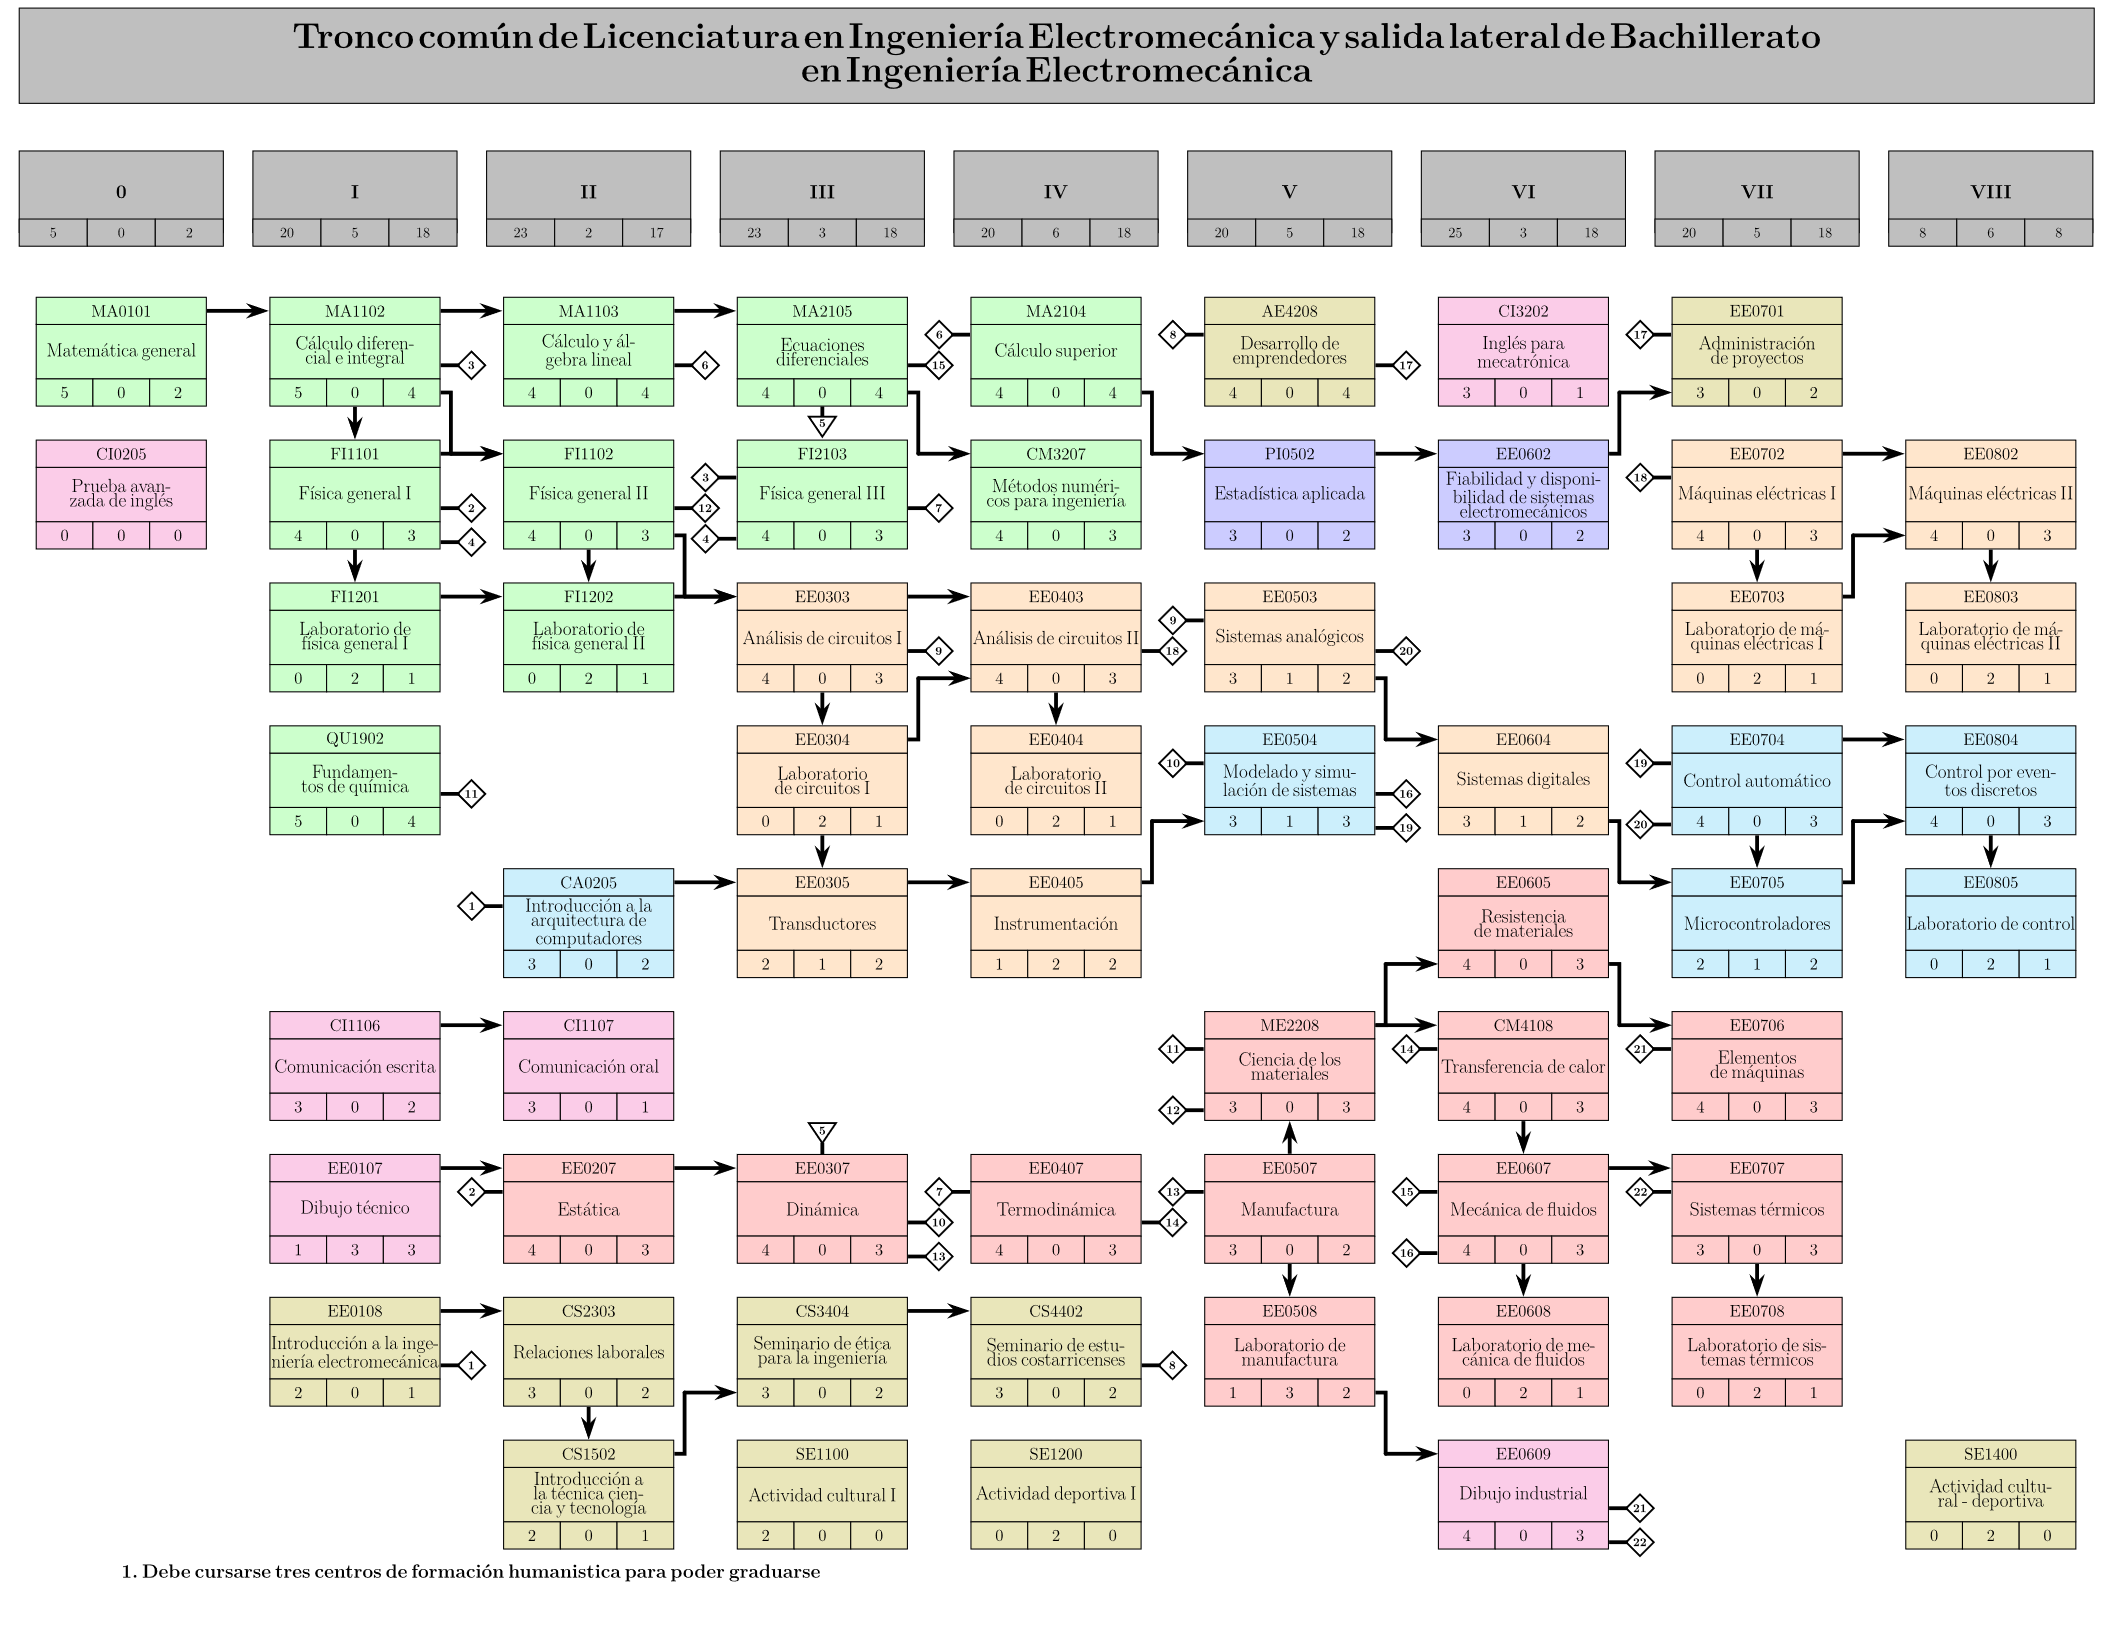
\includegraphics[width=\textwidth,height=.78\textheight,keepaspectratio]{figuras/figura_769.png}
\end{figure}

\subsection*{Malla curricular de la Licenciatura en Electromecánica con énfasis en Instalaciones electromecánicas}

\begin{figure}[htbp]
\centering
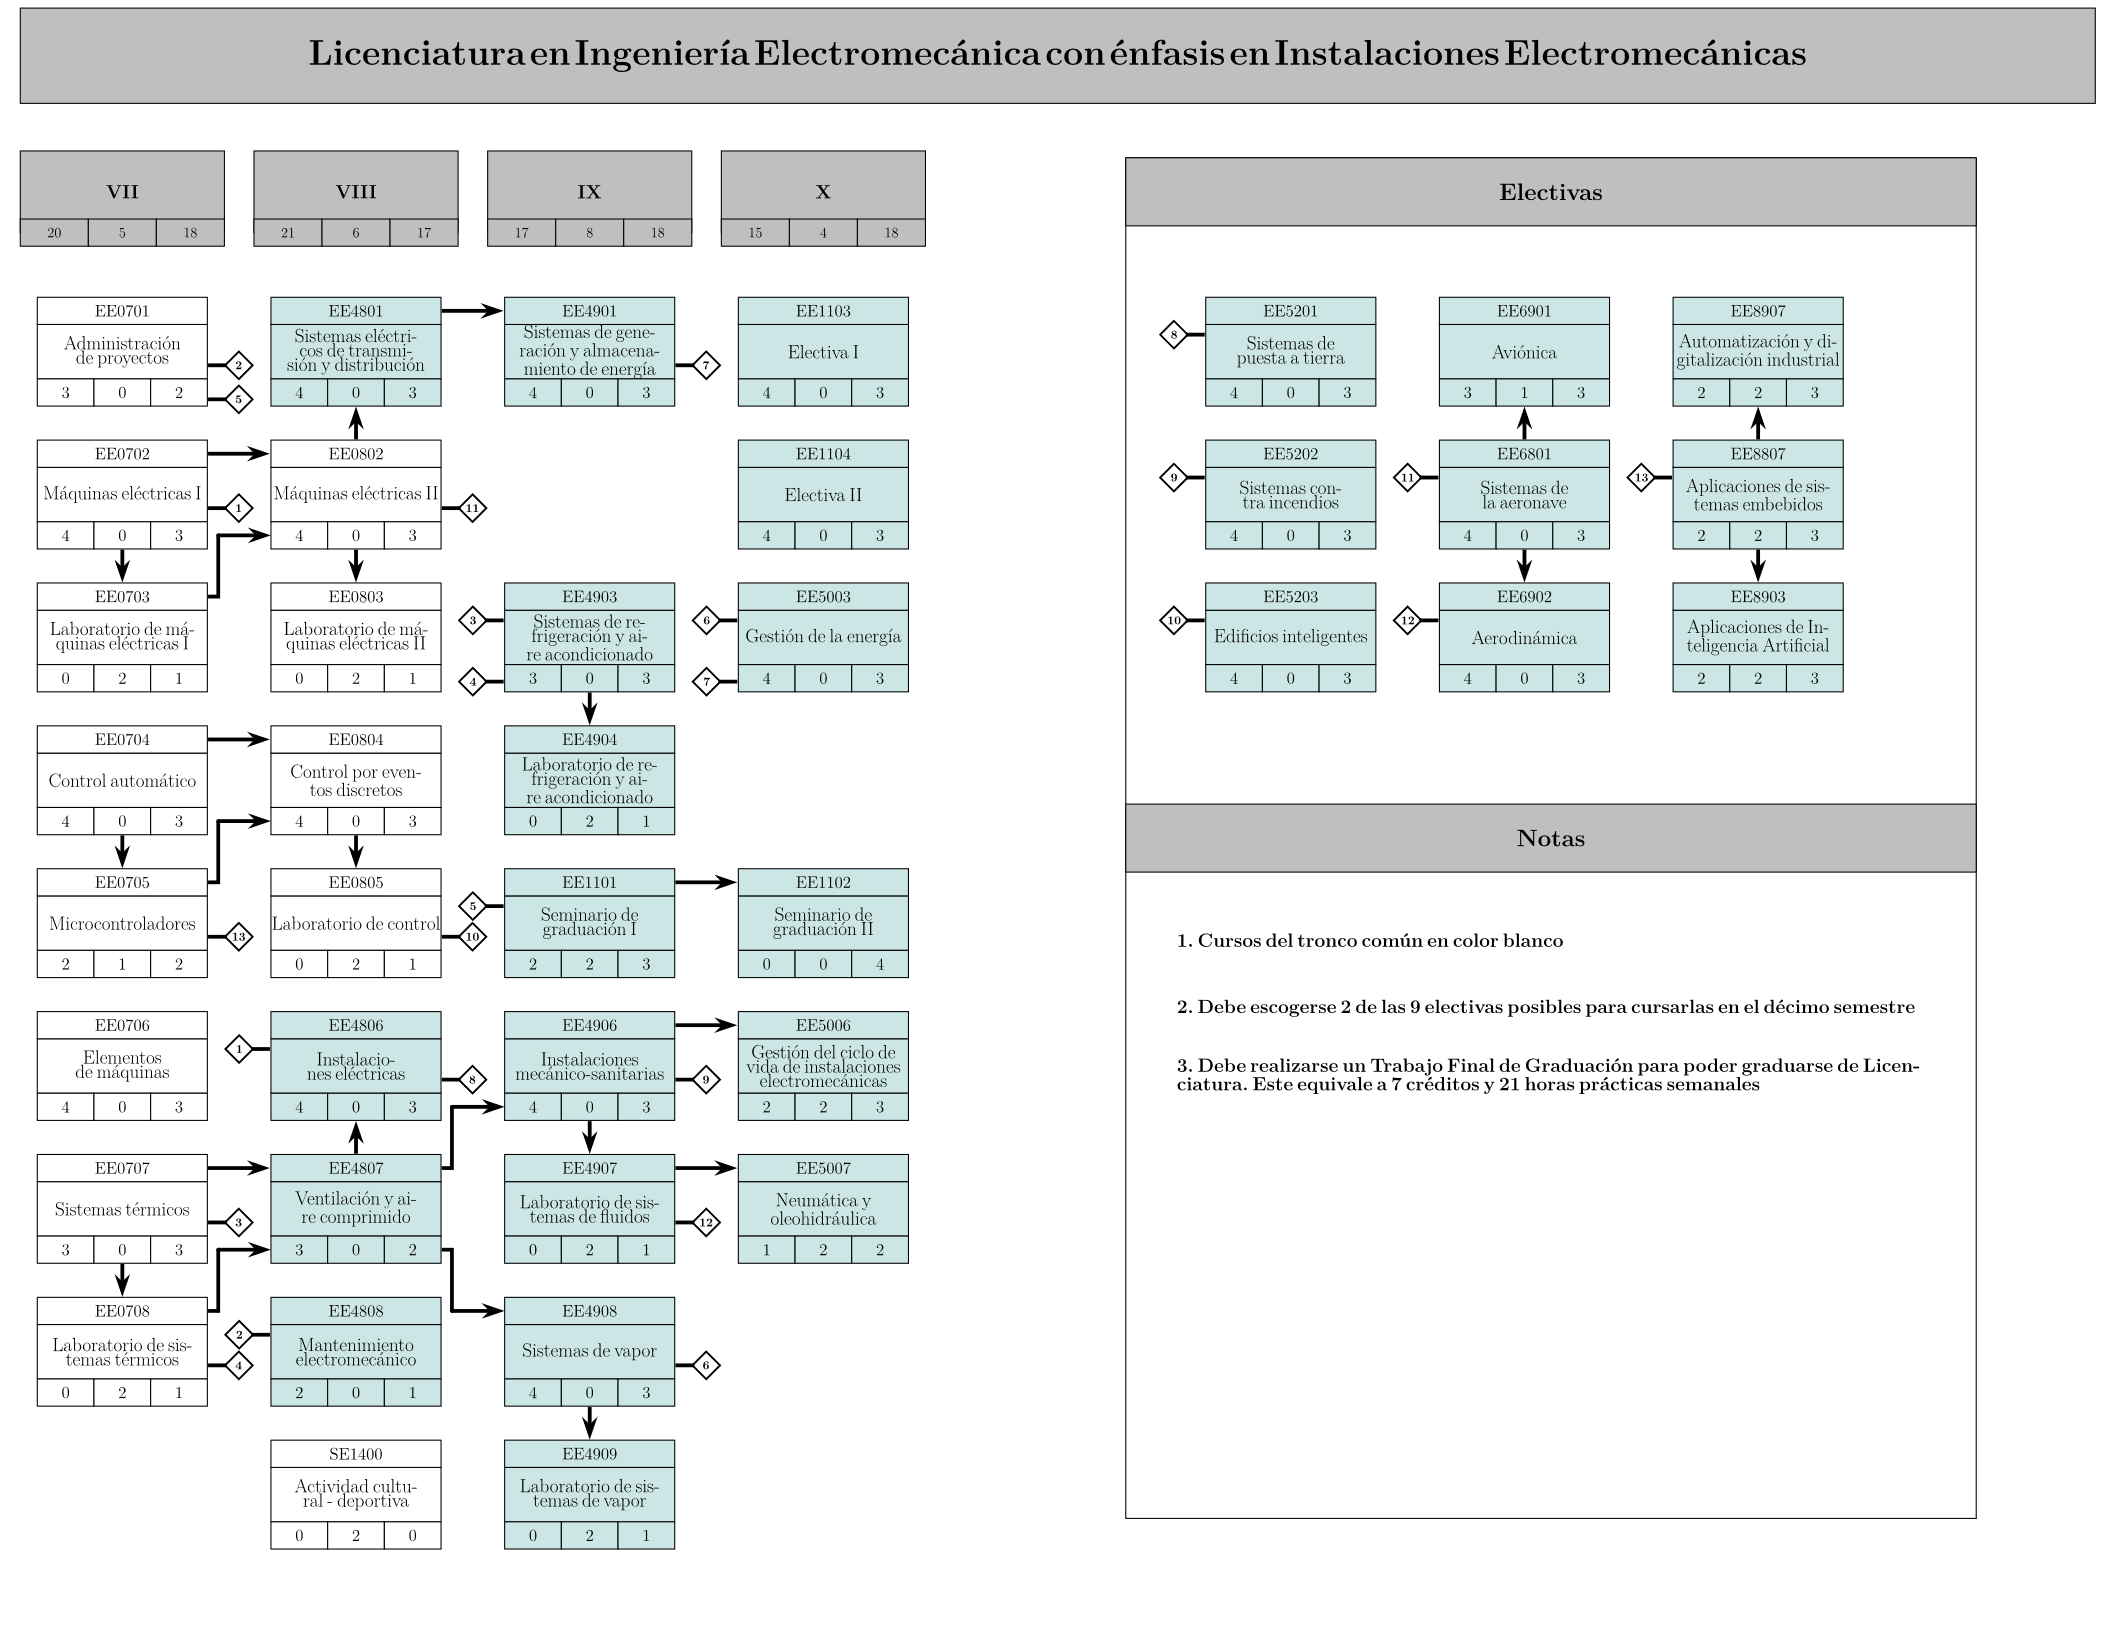
\includegraphics[width=\textwidth,height=.78\textheight,keepaspectratio]{figuras/figura_773.png}
\end{figure}

\subsection*{Malla curricular de la Licenciatura en Electromecánica con énfasis en Aeronáutica}

\begin{figure}[htbp]
\centering
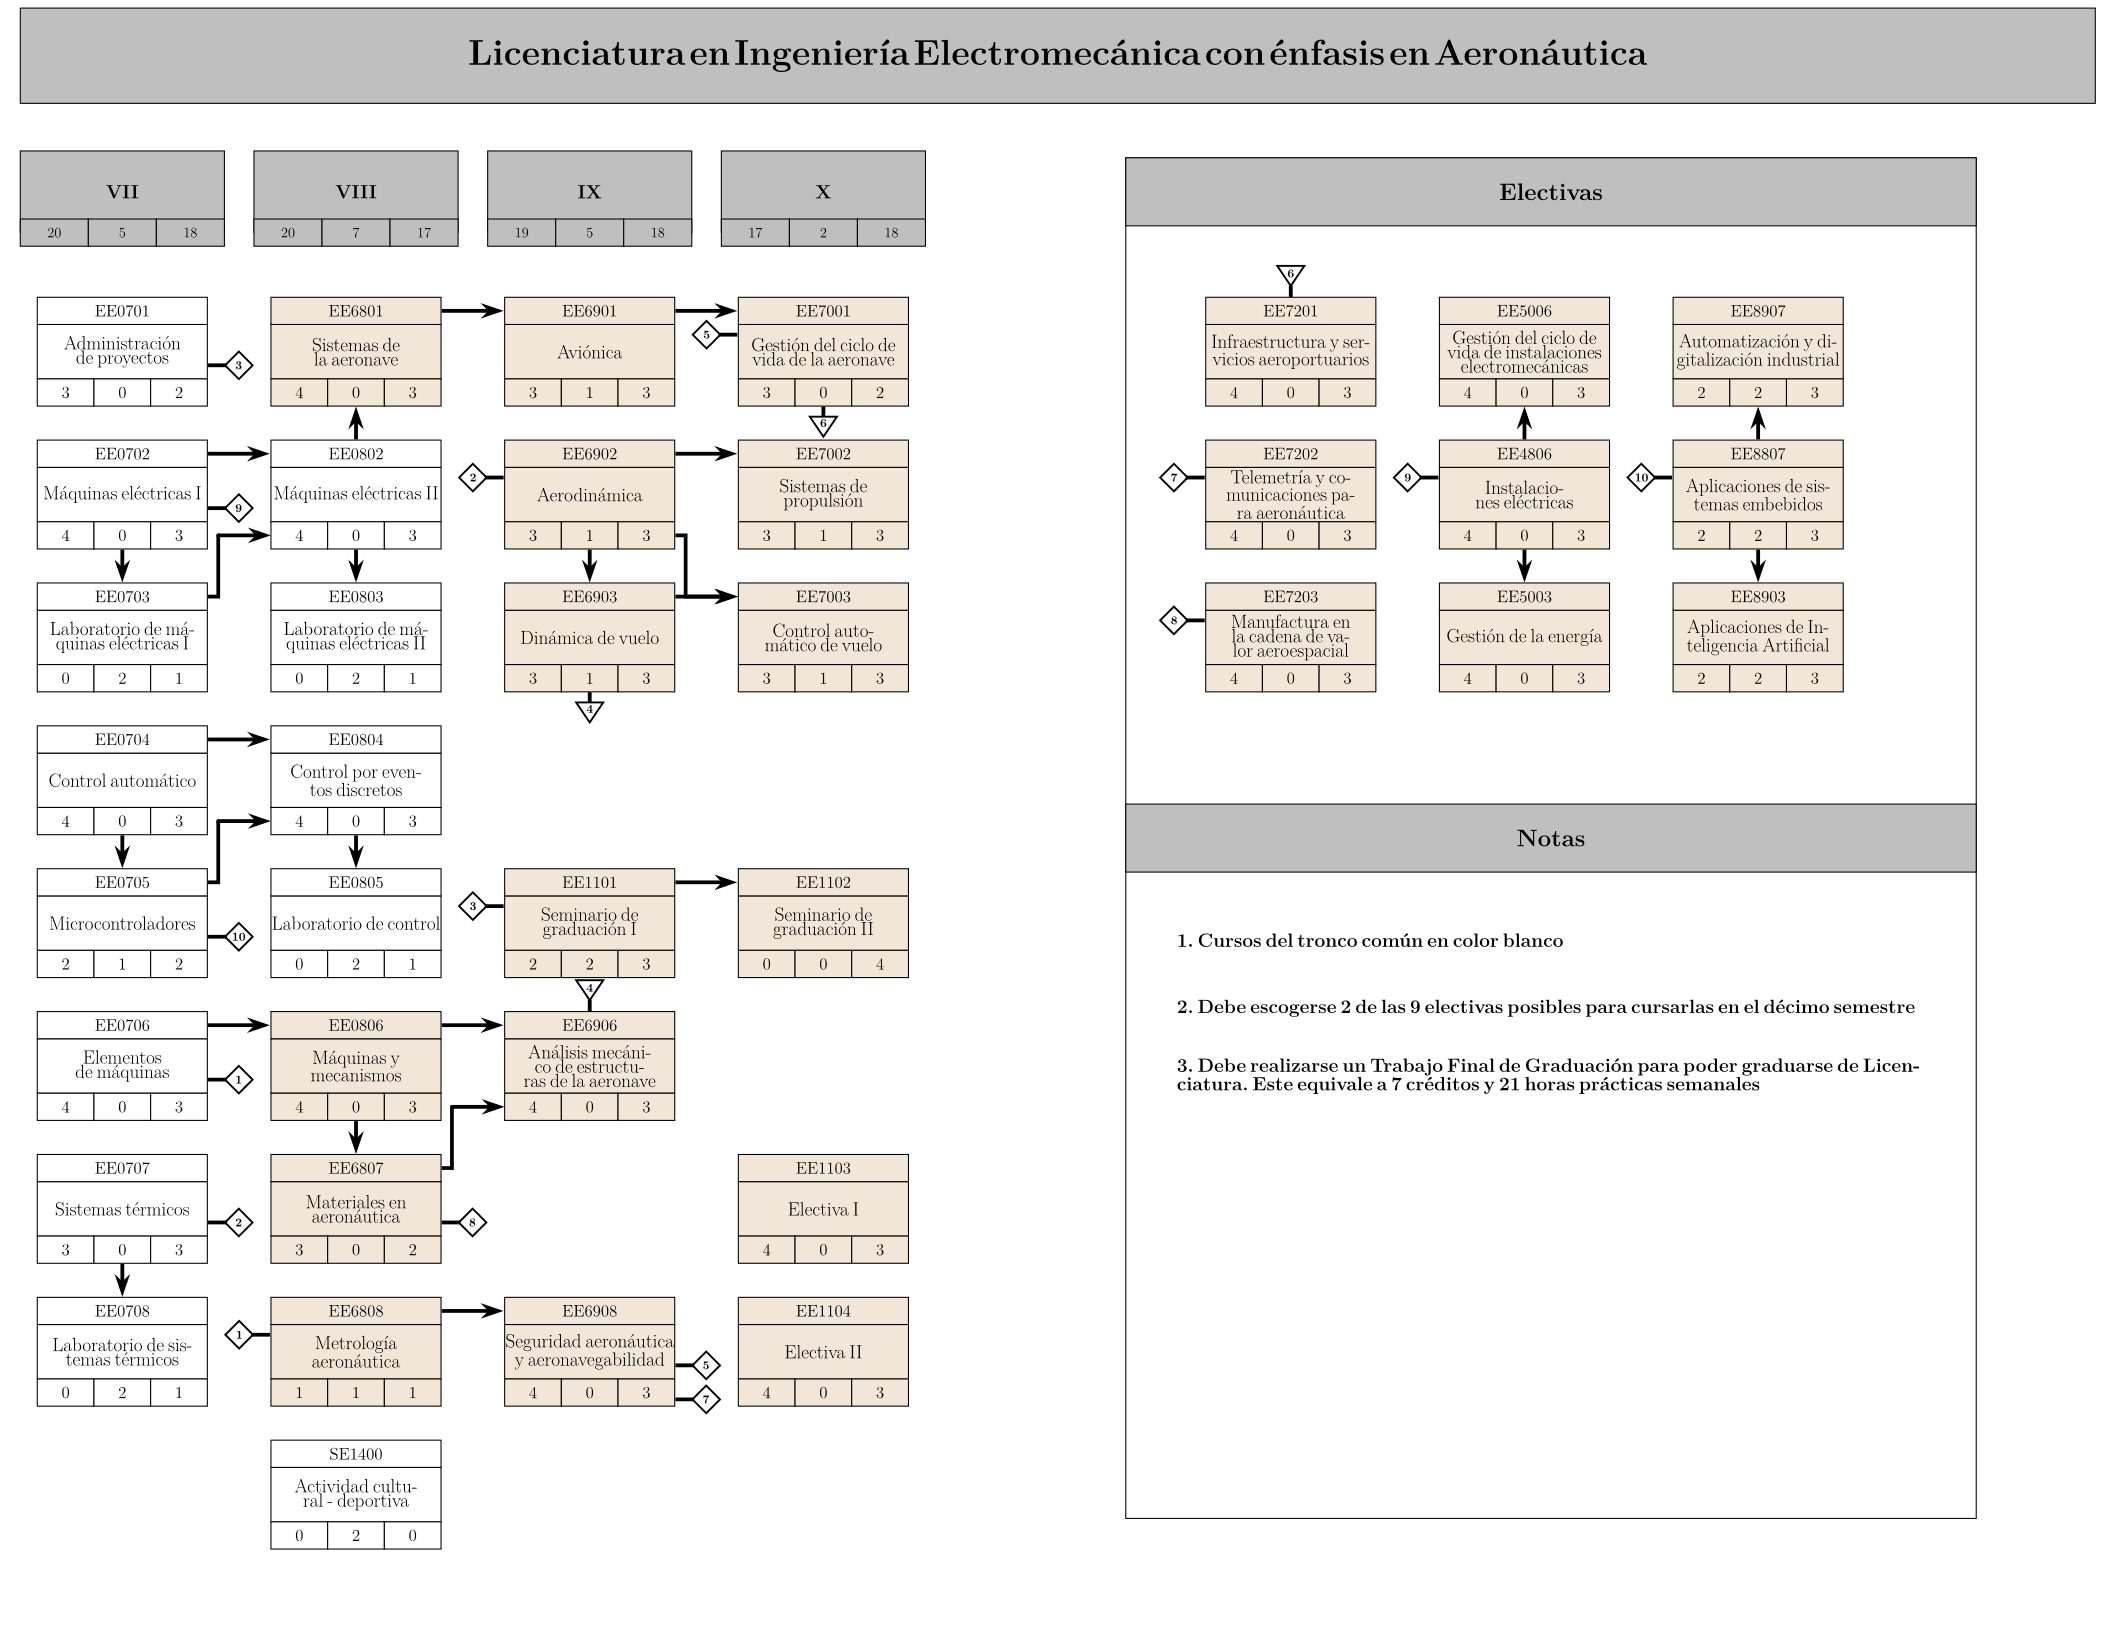
\includegraphics[width=\textwidth,height=.78\textheight,keepaspectratio]{figuras/figura_777.png}
\end{figure}

\subsection*{Malla curricular de la Licenciatura en Electromecánica con énfasis en Sistemas ciberfísicos}

\begin{figure}[htbp]
\centering
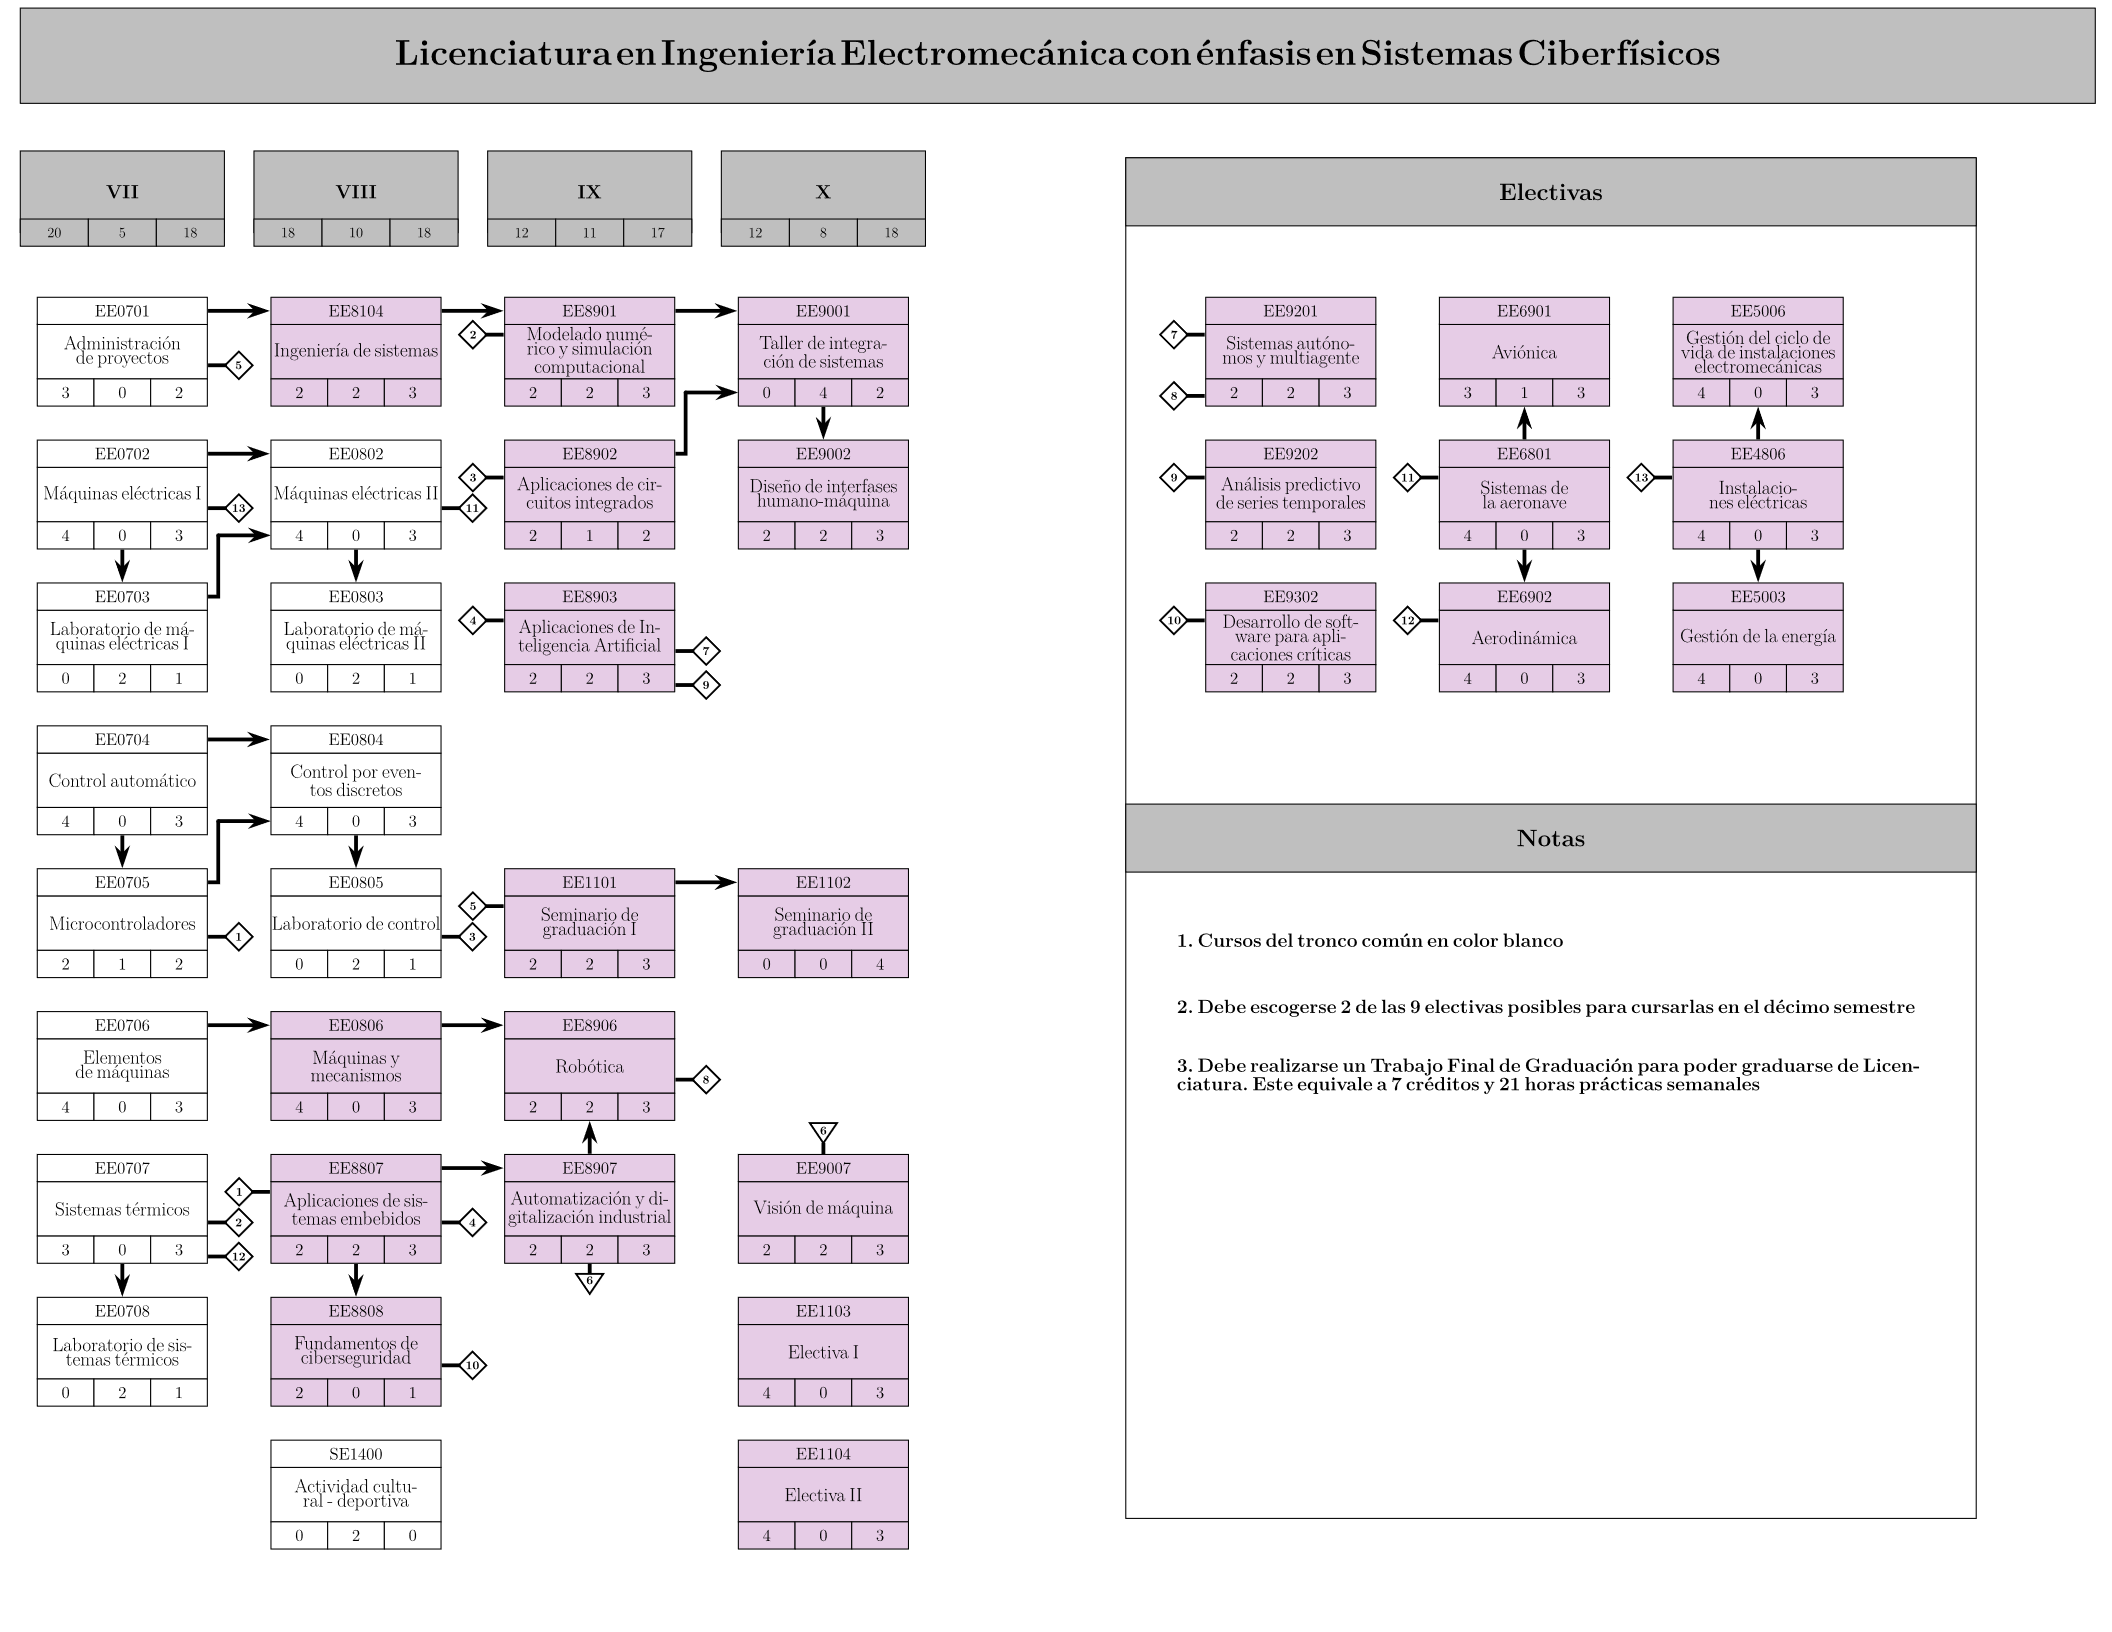
\includegraphics[width=\textwidth,height=.78\textheight,keepaspectratio]{figuras/figura_781.png}
\end{figure}

\section*{Requisitos}

\subsection*{Requisitos de ingreso}

Los requisitos de ingreso a la Licenciatura en Ingeniería en Electromecánica en cualquiera de sus tres énfasis están regulados en el \textit{Reglamento }\textit{de admisión a carreras de grado en el Instituto Tecnológico de Costa Rica}, se incluyen los artículos más relevantes:\par

\textit{\textbf{Artículo 17. Condiciones para inscribirse al proceso de admisión}}\par

\textit{La persona interesada en inscribirse al proceso de admisión debe cumplir}\textit{ }\textit{con alguna de las siguientes condiciones:}\textit{ }\par

\textit{a. Que se encuentre cursando el último año de la Educación}\textit{ }\textit{Diversificada.}\par

\textit{b. Que haya finalizado sus estudios secundarios dentro del sistema}\textit{ }\textit{de Educación Formal o Educación Abierta o que tenga posibilidad de}\textit{ }\textit{finalizarlos para el periodo de matrícula.}\textit{ }\par

\textit{c. Que haya obtenido el Certificado de Conclusión de Estudios}\textit{ }\textit{Secundarios o se encuentre cursando el último año de estos, en}\textit{ }\textit{cualquier otro país y presente los atestados correspondientes para}\textit{ }\textit{probarlo.}\par

\textit{\textbf{Artículo 13. Sobre el ingreso}}\par

\textit{La persona que desee solicitar el ingreso a las carreras de grado que oferta el Instituto Tecnológico de Costa Rica puede hacerlo por medio de alguna de las siguientes modalidades:}\par

\textit{a. Puntaje de admisión (Abierta, Restringida y Revalidación)}\par

\textit{b. Exención de puntaje de admisión}\par

\textit{c. Convenios de admisión vigentes autorizados por el Consejo}\textit{ }\textit{Institucional}\par

\textit{d. Otras que apruebe el Consejo Institucional}\par

\textit{\textbf{Artículo 14. Formalización del ingreso}}\par

\textit{La persona que desee formalizar su ingreso al Instituto Tecnológico de}\textit{ }\textit{Costa Rica debe:}\par

\textit{a. Haber sido declarada admitida según la modalidad de admisión}\textit{ }\textit{correspondiente.}\par

\textit{b. Matricular en la hora y día en que el Departamento de Admisión y}\textit{ }\textit{Registro le indique.}\par

\textit{c. Presentar todos los documentos requeridos en el formato definido}\textit{ }\textit{por el Departamento de Admisión y Registro.}\par

\subsection*{Aprobación de cursos y permanencia en la carrera}

La aprobación de cursos está regulada por el \textit{Reglamento al}\textit{ R}\textit{égimen de }\textit{E}\textit{nseñanza}\textit{-}\textit{A}\textit{pre}\textit{ndizaje del Instituto Tecnológico de Costa Rica}, en general para que un estudiante pueda aprobar un curso debe obtener una calificación alfabética AP (aprobado) y una calificación numérica mayor a setenta. Se incluyen los artículos correspondientes:\par

\textit{\textbf{Artículo 74. De la calificación alfabética final }}\par

\textit{La calificación alfabética describe el resultado del proceso de enseñanza y aprendizaje obtenido por la persona estudiante mediante una abreviatura, la cual se emplea para asignaturas específicas dentro del plan de estudios, previamente definidas por la dependencia o la }\textit{subdependencia}\textit{. Esta se consigna }\textit{con una de las siguientes abreviaturas en el acta de calificaciones finales del curso: AP (aprobado), RP (reprobado), IN (incompleto) o RPA (reprobado por ausencias).   }\par

\textit{\textbf{Artículo 75. De la calificación numérica final de aprobación   }}\par

\textit{La calificación numérica final mínima para aprobación de una asignatura, una vez aplicado el redondeo respectivo, será de setenta. Esta se obtendrá mediante un promedio ponderado de las calificaciones parciales, cuyo valor esté definido en el programa de la asignatura.  }\par

\textit{\textbf{Artículo 78. De la evaluación de reposición}}\par

\textit{La persona estudiante tendrá derecho a presentar una evaluación de reposición de la asignatura cuya nota final sea 60 o 65, una vez aplicado el redondeo. Se exceptuarán los laboratorios, talleres, seminarios, cursos de casos y proyectos, y demás asignaturas así definidas por el Consejo de Departamento respectivo, con anterioridad al inicio del curso, así como las asignaturas impartidas en el periodo de cursos de verano.  }\par

\textit{La persona estudiante aprobará la asignatura, si en el examen de reposición obtiene una calificación mayor o igual a 70, en cuyo caso la nota final de la asignatura será igual a 70. En caso contrario, su nota será la obtenida antes del examen de reposición. }\par

\textit{\textbf{Artículo 83. De la reprobación por ausencias  }}\par

\textit{La persona estudiante que acumule hasta un 15\% de ausencias en un curso de asistencia obligatoria se considerará reprobada y, para los efectos de actas de calificaciones, la asignatura aparecerá con las siglas RPA (Reprobado por ausencias) y con la nota que le corresponda de acuerdo con los criterios de evaluación establecidos para dicho curso.  }\par

\textit{Se exceptuarán aquellos casos de personas estudiantes próximas a graduarse que trabajan y con quienes la persona docente haya acordado ajustes operativos (metodológicos y evaluativos) debido a su condición de haber reprobado dos o más veces la asignatura, o según lo indicado en este reglamento sobre las actividades prácticas. Estos ajustes acordados deberán constar por escrito.  }\par

Respecto a la permanencia, \textit{el Reglamento al Régimen de Enseñanza-Aprendizaje del Instituto Tecnológico de Costa Rica} establece:\par

\textit{\textbf{Artículo 20. De la pérdida de condición de estudiante regular o especial   }}\par

\textit{Las personas estudiantes regulares y especiales perderán esta condición cuando: }\par

\textit{a. No lleven a cabo los trámites de matrícula correspondientes al período lectivo en curso y no tengan en proceso la culminación de cursos en los cuales se haya dado la condición de IN (incompleto). }\par

\textit{b. Se compruebe la falsedad de datos necesarios para el empadronamiento y la matrícula.          }\par

\textit{c. Hayan tramitado el retiro de todos los cursos matriculados, de acuerdo con las normas establecidas en este Reglamento.   }\par

\textit{d. Por motivos de fuerza mayor debidamente justificados, hayan tramitado la interrupción de estudios.     }\par

\textit{e. De conformidad con los procedimientos establecidos por la Institución, se haya dictado una separación temporal de esta, por un período igual o mayor a un semestre lectivo.   }\par

\textit{f. Se haya graduado. }\par

\subsection*{Reingresos}

Los reingresos están regulados por el \textit{R}\textit{eglamento de Admisión a Carreras de Grado en el Instituto Tecnológico de Costa Rica}, los estudiantes que opten por la salida lateral de Bachillerato y deseen reingresar después de haber perdido la condición de estudiante regular deben realizar el proceso conforme a este reglamento. Se incluyen los artículos correspondientes:\par

\textit{\textbf{Artículo 34.  Solicitud de reingreso  }}\par

\textit{La persona estudiante que desee reingresar al ITCR después de haber suspendido sus estudios por un periodo lectivo o más, deberá presentar la solicitud según el procedimiento definido por el Departamento de Admisión y Registro y durante el período establecido para tal efecto en el Calendario Institucional }\par

\textit{\textbf{Artículo 35. Requisito para solicitar reingreso }}\par

\textit{Tendrá derecho a reingresar a la carrera la persona estudiante que haya aprobado como mínimo dos créditos del plan de estudios de la carrera en que estuvo inscrito, siempre y cuando la carrera se encuentre activa y cumpla con los requisitos adicionales de admisión a la carrera que estén vigentes al momento de realizar el reingreso. }\par

\textit{\textbf{Artículo 36.  Puntaje de ingreso para los reingresos}}\par

\textit{A quien solicite reingresar al ITCR, se le tomará en cuenta como puntaje de ingreso el promedio ponderado de las calificaciones correspondientes al último periodo cursado. }\par

\textit{\textbf{Artículo 37. Vigencia del plan de estudios para los reingresos }}\par

\textit{A la persona que se le apruebe el reingreso a carrera se le incluirá en el plan de estudios que se encuentre vigente en ese momento. Si el plan de estudios en el que estuvo anteriormente ha sufrido cambios, la equivalencia de los cursos que tenga aprobados deberán ajustarse a lo que haya acordado el Consejo de Docencia.}\par

\subsection*{Actividades de nivelación}

Al respecto de estas actividades, el \textit{R}\textit{eglamento al R}\textit{égimen de Enseñanza-Aprendizaje del Instituto Tecnológico de Costa Rica}, indica que:\par

\textit{\textbf{Artículo 23. De las actividades de nivelación  }}\par

\textit{Para el estudiantado de primer ingreso que, mediante estudios, se detecte que presentan deficiencia en conocimientos básicos, se programarán asignaturas y actividades tendientes a la nivelación o al logro de un mejor ajuste al sistema académico del plan de estudios. Estas actividades no estarán incluidas en los planes de estudio, no recibirán créditos y serán requisito de los cursos para los cuales se detectó la necesidad.   }\par

\textit{Para estudiantes de grado, la asistencia a algunas de estas asignaturas o actividades podrán ser de carácter obligatorio, cuando así lo establezca mediante resolución fundamentada la persona titular de la Vicerrectoría de Docencia.}\par

\textit{Para estudiantes que ingresan bajo la modalidad de Admisión Restringida, la asistencia a las actividades de nivelación tendrá carácter de obligatoriedad según su normativa.  }\par

\textit{En el caso de estudiantes de posgrado, estas asignaturas podrán ser de carácter obligatorio cuando así lo establezca el Área Académica o la Unidad de Posgrado, al definir los requisitos de ingreso de su plan de estudio o mediante resolución fundamentada}\par

\subsection*{Requisitos de graduación y nombre del título a otorgar}

Para graduarse obteniendo la salida lateral de bachillerato se requiere aprobar todos los cursos del plan de estudios que corresponden al tronco común, además de los 3 centros de Formación Humanística y para graduarse de la licenciatura se requiere aprobar los cursos del tronco común mas todos los cursos de alguno de los tres énfasis por el cual opto y realizar un Trabajo Final de Graduación. Los requisitos de graduación están normados en el Reglamento de Normas Generales de Graduación en el Tecnológico de Costa Rica:\par

\textit{\textbf{Artículo 5}}\par

\textit{Los requisitos indispensables para obtener el diploma del Instituto son los siguientes:}\par

\textit{a. Haber cumplido con el programa de estudios correspondientes a alguna de las carreras que se imparten en el Instituto.}\par

\textit{b. No estar cumpliendo con algún tipo de sanción académica o disciplinaria, impuesta por alguna dependencia competente del Instituto.}\par

\textit{c. Solicitar la expedición de su diploma al Departamento de Admisión y Registro en las fechas establecidas para ese efecto y según el trámite que se le indique.}\par

\textit{d. No tener compromisos con la Institución.}\par

El titulo a otorgar es:\par

\begin{itemize}
\item En la salida lateral de bachillerato:
\begin{itemize}
\item Bachillerato Universitario en Ingeniería Electromecánica
\end{itemize}
\item Licenciatura:
\begin{itemize}
\item Licenciatura en Ingeniería Electromecánica con énfasis en Instalaciones Electromecánicas
\item Licenciatura en Ingeniería Electromecánica con énfasis en Aeronáutica
\item Licenciatura en Ingeniería Electromecánica con énfasis en Sistemas Ciberfísicos
\end{itemize}
\end{itemize}
\section*{Administración curricular y organización}

\subsection*{Administración curricular}

El \textit{Reglamento para el diseño y rediseño curricular de los planes de estudio pregrado y grado en el ITCR} establece una serie de lineamientos que definen como se administran los procesos de planificación, diseño, evaluación, gestión y mejoramiento continuo del plan de estudios, esto se aclara en su alcance:\par

\textit{\textbf{Artículo 2. Del alcance del reglamento }}\par

\textit{El presente reglamento es de acatamiento obligatorio para los responsables de las escuelas o áreas académicas en la formulación, aprobación, ejecución o administración curricular de cursos y planes de estudio, con la asesoría académica técnico-curricular del CEDA.}\par

Las responsabilidades de los actores dentro de la Escuela que administra el plan de estudios están definidas en los siguientes artículos:\par

\textit{\textbf{Artículo 8. Responsabilidades de la persona en la dirección de escuela o coordinación de área académica}}\par

\textit{Para efectos de este reglamento, la persona en la dirección de la escuela o coordinación de área académica tendrá las siguientes responsabilidades específicas:}\par

\textit{a) Proponer al Consejo de Escuela o Área Académica, según corresponda, los miembros que conformarán la Comisión Curricular. }\par

\textit{b) Gestionar el acompañamiento y colaboración de una persona asesora académica ante la dirección del CEDA en los procesos de diseño y rediseño de los programas del curso y planes de estudio.}\par

\textit{c) Gestionar en primera instancia las propuestas de diseño o rediseño curricular de los cursos o planes de estudio ante el Consejo de escuela o área académica apoyado por la Comisión Curricular.}\par

\textit{d) Solicitar a la dirección del CEDA el dictamen con el análisis especializado oficial (positivo o negativo), junto al informe con criterio académico técnico curricular }\textit{recomendativo}\textit{ de diseño o rediseño emitido por la persona asesora académica una vez concretada la propuesta de diseño o rediseño curricular de planes de estudio o cursos.}\par

\textit{e) Gestionar, ante las instancias correspondientes, las propuestas de diseño o rediseño curricular de los planes de estudios o cursos. }\par

\textit{f) Propiciar la coordinación de las propuestas de diseño o rediseño curricular de los planes de estudio o cursos con las de otras escuelas o áreas del Instituto.}\par

\textbf{Artículo 9. Responsabilidades del Consejo de Escuela o Área Académica}\par

\textit{Para efectos de este reglamento, el Consejo de Escuela o Área Académica}\textit{ }\textit{tendrá las siguientes responsabilidades específicas:}\textit{ }\par

\textit{a) Nombrar la Comisión Curricular de la Escuela o Área Académica que se}\textit{ }\textit{encargará de realizar los procesos de diseño y rediseño curricular de los}\textit{ }\textit{planes de estudio o cursos.}\par

\textit{b) Dar seguimiento a los avances de la Comisión Curricular de acuerdo con}\textit{ }\textit{su nombramiento y funciones.}\par

\textit{c) Aprobar o rechazar en primera instancia sobre las propuestas de diseño}\textit{ }\textit{o rediseño curricular de los planes de estudio o cursos.}\par

\textit{d) Elevar}\textit{ }\textit{al Consejo de Docencia la propuesta de diseño o rediseño}\textit{ }\textit{curricular de los planes de estudio o cursos.}\par

\textit{e) Solicitar el traslado, cierre o eliminación de planes de estudio para su}\textit{ }\textit{aprobación o rechazo, ante las instancias según corresponda}\par

\textit{\textbf{Artículo 7. Responsabilidades de la Comisión Curricular}}\par

\textit{Cada escuela o área académica contará con una comisión curricular para el}\textit{ }\textit{diseño o rediseño curricular y tendrá las siguientes funciones:}\textit{ }\par

\textit{a) Revisar y analizar sistemáticamente oportunidades de mejora en cuanto}\textit{ }\textit{al diseño o rediseño curricular de los planes de estudio que le}\textit{ }\textit{corresponden.}\par

\textit{b) Atender solicitudes designadas por el Consejo de Escuela o Consejo de}\textit{ }\textit{Área Académica para la revisión de programas del curso, diseño o}\textit{ }\textit{rediseño de planes de estudio según la estructura administrativa de}\textit{ }\textit{gestión académica interna establecida.}\par

\textit{c) Elaborar en conjunto con la asesoría académica del CEDA, las}\textit{ }\textit{propuestas de diseño o rediseño curricular de los planes de estudios o}\textit{ }\textit{cursos.}\par

\textit{d) Apoyar}\textit{ }\textit{a la dirección de escuela o coordinación de área académica en}\textit{ }\textit{la exposición y argumentación de las propuestas de diseño o rediseño}\textit{ }\textit{curricular de los planes de estudios ante los Consejos de Escuelas o}\textit{ }\textit{Consejos de Áreas Académicas institucionales e interinstitucionales.}\par

\textit{e) Dar seguimiento a las decisiones del Consejo de Escuela o Área}\textit{ }\textit{Académica en cuanto a la creación, diseño o rediseño curricular de los}\textit{ }\textit{planes de estudio o cursos.}\par

\subsection*{Organización}

Considerando que los procesos de planificación, diseño, evaluación, gestión y mejoramiento continuo del plan de estudios incluyen inclusive los procesos de acreditación, se plantea la creación de una Comisión permanente de asuntos académicos que administre los procesos relacionados al plan de estudios, incluido lo relacionado con acreditación.\par

Además, se propone la distribución del cuerpo docente en cinco foros de área curricular que faciliten un espacio de discusión de mejoras curriculares que puedan plantearse a la comisión curricular permanente. Los foros son convocados por la Comisión de asuntos académicos y son coordinados por el representante del foro en la Comisión. El coordinador debe llevar propuestas construidas en el seno del foro a la comisión curricular para que la comisión curricular realice el trabajo de darles contenido, consensuarlas internamente y llevarlas al Consejo de Escuela.\par

Al menos una vez cada dos años el Consejo de Escuela debe acreditar la formación de los profesores en las áreas disciplinares del programa en Ingeniería Electromecánica, que son las siguientes:\par

\begin{itemize}
\item Formación profesional y habilidades interpersonales
\item Comunicación y dibujo
\item Ingeniería eléctrica y electrónica
\item Ingeniería mecánica y de materiales
\item Automática
\item Análisis de datos Instalaciones electromecánicas
\item Aeronáutica
\item Sistemas ciberfísicos
\end{itemize}
\begin{figure}[htbp]
\centering
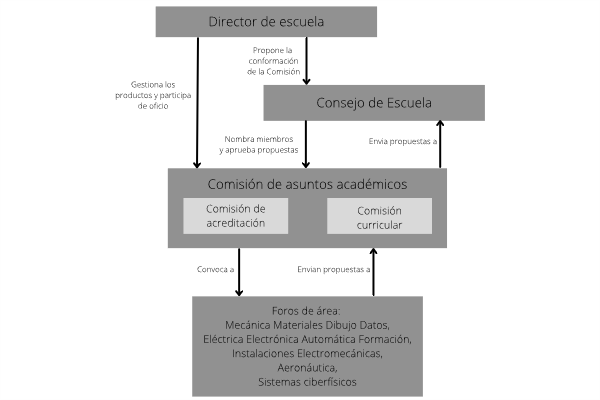
\includegraphics[width=\textwidth,height=.78\textheight,keepaspectratio]{figuras/figura_899.png}
\par\vspace{2mm}
{\centering\small Figura 8. Organización de la Escuela de Ingeniería Electromecánica para facilitar la administración curricular\par}
\end{figure}

\subsection*{Comisión de asuntos académicos}

Estará conformada por siete personas según la siguiente distribución:\par

\begin{itemize}
\item El director de la Escuela de Ingeniería Electromecánica
\item El coordinador de los seminarios y el trabajo final de graduación
\item Un profesor con formación en al menos dos de las siguientes áreas:
\begin{itemize}
\item Ingeniería mecánica y de materiales
\item Comunicación y dibujo
\item Análisis de datos
\end{itemize}
\item Un profesor con formación en al menos dos de las siguientes áreas:
\begin{itemize}
\item Ingeniería eléctrica y electrónica
\item Automática
\item Formación profesional y habilidades interpersonales
\end{itemize}
\item Un profesor con formación en el área de instalaciones electromecánicas
\item Un profesor con formación en el área de aeronáutica
\item Un profesor con formación en el área de sistemas ciberfísicos
\item Una persona estudiante como representación estudiantil
\end{itemize}
Con excepción del director de Escuela que participa en la comisión de oficio, los demás integrantes deberán ser elegidos por el Consejo de Escuela a partir de una recomendación del director.\par

\subsection*{Foro de áreas Mecánica-Materiales-Dibujo-Datos}

Conformado por las personas docentes a los que el Consejo de Escuela a designado como profesionales con formación en los siguientes saberes:\par

\begin{itemize}
\item Ciencia e ingeniería de los materiales
\item Mecánica de sólidos y fluidos
\item Termodinámica y transferencia de calor
\item Elementos de máquinas
\item Manufactura
\item Dibujo para ingeniería
\item Estadística y diseño de experimentos
\item Confiabilidad, disponibilidad, mantenibilidad y seguridad
\item Metrología
\end{itemize}
El grupo de personas docentes pertenecientes a este foro debe participar activamente en la administración curricular de cursos propios pertenecientes a las siguientes áreas curriculares:\par

\begin{itemize}
\item Ingeniería mecánica y de materiales
\item Comunicación y dibujo
\item Análisis de datos
\end{itemize}
\subsection*{Foro de área curricular Eléctrica-Electrónica-Automática-Formación}

Conformado por las personas docentes a los que el Consejo de Escuela a designado como profesionales con formación en los siguientes saberes:\par

\begin{itemize}
\item Circuitos eléctricos y electrónica
\item Máquinas eléctricas
\item Instrumentación y transductores
\item Programación
\item Modelado y simulación
\item Microcontroladores y arquitectura de computadores
\item Sistemas de control y automatización
\item Administración de proyectos
\end{itemize}
El grupo de personas docentes pertenecientes a este foro debe participar activamente en la administración curricular de cursos propios pertenecientes a las siguientes áreas curriculares:\par

\begin{itemize}
\item Ingeniería eléctrica y electrónica
\item Automática
\item Formación profesional y habilidades interpersonales
\end{itemize}
\subsection*{Foro de área curricular Instalaciones Electromecánicas}

Conformado por las personas docentes a los que el Consejo de Escuela a designado como profesionales con formación en los siguientes saberes:\par

\begin{itemize}
\item Instalaciones electromecánicas
\item Sistemas de generación y almacenamiento de energía
\item Sistemas de distribución y transmisión de energía eléctrica
\item Gestión del ciclo de vida y transformación digital
\item Gestión de la energía
\end{itemize}
El grupo de personas docentes pertenecientes a este foro debe participar activamente en la administración curricular de cursos propios pertenecientes al área curricular:\par

\begin{itemize}
\item Instalaciones electromecánicas
\end{itemize}
\subsection*{Foro de área curricular Aeronáutica}

Conformado por las personas docentes a los que el Consejo de Escuela a designado como profesionales con formación en los siguientes saberes:\par

\begin{itemize}
\item Aviónica, dinámica de vuelo y control de vuelo
\item Aerodinámica y sistemas de propulsión
\item Análisis mecánico de materiales, estructuras y mecanismos de la aeronave
\item Gestión del ciclo de vida de la aeronave
\item Seguridad aeronáutica y aeronavegabilidad.
\end{itemize}
El grupo de personas docentes pertenecientes a este foro debe participar activamente en la administración curricular de cursos propios pertenecientes al área curricular\par

\begin{itemize}
\item Aeronáutica
\end{itemize}
\subsection*{Foro de área curricular Sistemas Ciberfísicos}

Conformado por las personas docentes a los que el Consejo de Escuela a designado como profesionales con formación en los siguientes saberes:\par

\begin{itemize}
\item Aplicaciones de sistemas embebidos
\item Automatización y digitalización
\item Robótica
\item Modelado numérico y simulación computacional
\item Ingeniería de sistemas complejos
\item Aplicaciones de Inteligencia Artificial
\item Ciberseguridad
\end{itemize}
